% Se pre-carga la información del estudiante sólo para poder emplear el macro de
% selección de versión (digital o impresa)
\input{0-datos_estudiante}

\ifdefined\printver
    \documentclass[11pt, letterpaper, twoside, openright]{report}
\else
    \documentclass[11pt, letterpaper]{report}
\fi

% Eliminar la opción de twoside y openright si se desea generar la versión
% digital del documento en lugar de la versión impresa
%\documentclass[11pt, letterpaper, twoside, openright]{report}
\usepackage[spanish, es-nodecimaldot, es-noquoting]{babel}
% cambiar a spanish, mexico si se quiere emplear tabla en lugar de cuadro
\selectlanguage{spanish}
\usepackage[utf8]{inputenc}
\usepackage[T1]{fontenc}

\title{Plantilla para Trabajos de Graduación IE-MT 2019v3}
\author{MSc. Miguel Zea}
\date{\today}

% Información del estudiante en el archivo datos_estudiante.tex
\input{0-datos_estudiante}
\input{1-opciones_adicionales}
% fuerza input directo (sin macro) para que Synctex mapee bien
\let\parpordefecto\undefined

% ==============================================================================
% DEFINICIÓN DE PAQUETES
% ==============================================================================
\usepackage{xcolor}
\usepackage{amsfonts}
\usepackage{amsmath}
\usepackage{amssymb}
\usepackage{amsthm}
\usepackage{amsfonts}
\usepackage{mathtools}
\usepackage{graphicx}
\usepackage{xfrac}
\usepackage{float}
\usepackage{mathtools}
\usepackage[hidelinks,hypertexnames=false]{hyperref}
% Forzar ocultar bordes/colores de hipervínculos en todo el documento
\AtBeginDocument{%
  \hypersetup{
    hidelinks,
    colorlinks=false,
    linkcolor=black,
    urlcolor=black,
    citecolor=black,
    filecolor=black,
    runcolor=black,
    pdfborder={0 0 0},
    pdfborderstyle={/S/U/W 0}, % sin subrayado
    linkbordercolor={1 1 1},
    urlbordercolor={1 1 1},
    citebordercolor={1 1 1},
    filebordercolor={1 1 1},
    runbordercolor={1 1 1}
  }
}
% \usepackage{bookmark}
\usepackage[font=small]{caption}
\usepackage{subcaption}
\captionsetup{position=top,justification=raggedright,singlelinecheck=false}
\captionsetup[sub]{position=top,justification=raggedright,singlelinecheck=false}
\usepackage[titles]{tocloft}
\renewcommand{\cftfigpresnum}{Figura~}
\renewcommand{\cftfigaftersnum}{:}
\setlength{\cftfignumwidth}{6em} 

\renewcommand{\cfttoctitlefont}{\hfill\normalsize\bfseries}
\renewcommand{\cftaftertoctitle}{\hfill}
\renewcommand{\cftbeforetoctitleskip}{-1.0em}
\renewcommand{\cftaftertoctitleskip}{0.5em}

\renewcommand{\cftloftitlefont}{\hfill\normalsize\bfseries}
\renewcommand{\cftafterloftitle}{\hfill}
\renewcommand{\cftbeforeloftitleskip}{-1.0em}
\renewcommand{\cftafterloftitleskip}{0.5em}

\renewcommand{\cftlottitlefont}{\hfill\normalsize\bfseries}
\renewcommand{\cftafterlottitle}{\hfill}
\renewcommand{\cftbeforelottitleskip}{-1.0em}
\renewcommand{\cftafterlottitleskip}{0.5em}
%\usepackage{csquotes}
\usepackage{xpatch}
\usepackage{emptypage}
\usepackage{hyphenat}
\usepackage{fancyhdr}
\usepackage[backend=biber, style=ieee]{biblatex}
\ifdefined\usarAPA 
    \usepackage[backend=biber, style=apa]{biblatex}
\fi
\addbibresource{o-bibliografia.bib}

\usepackage[percent]{overpic}

\usepackage{chngcntr}

\ifdefined\CAPglosario
	\usepackage[numberedsection,toc]{glossaries}
	\makenoidxglossaries
	\renewcommand*{\glossentryname}[1]{\glsnamefont{\glsentryname{#1}:}}
    % p-glosario.tex
% !TEX root = z-main.tex

\newglossaryentry{3d}{
    name={3D},
    description={Término que se refiere a representaciones tridimensionales, es decir, con ancho, alto y profundidad}
}

\newglossaryentry{RA}{
    name={RA},
    description={Acrónimo de Realidad Aumentada, tecnología que superpone elementos digitales en el entorno físico del usuario}
}

\newglossaryentry{RV}{
    name={RV},
    description={Acrónimo de Realidad Virtual, tecnología que sumerge al usuario en un entorno digital completamente generado por computadora}
}

\newglossaryentry{ARCore}{
    name={ARCore},
    description={Plataforma de desarrollo de realidad aumentada creada por Google, que permite construir aplicaciones que integran elementos digitales en el mundo real}
}

\newglossaryentry{Wireframe}{
    name={Wireframe},
    description={Representación visual de un modelo tridimensional utilizando líneas y aristas para mostrar su estructura básica sin superficies sólidas}
}

\newglossaryentry{pipeline}{
    name={pipeline},
    description={Conjunto de procesos y etapas secuenciales que se siguen para lograr un objetivo específico, como la creación de modelos 3D o el desarrollo de software}
}


\newglossaryentry{PBR}{
    name={PBR},
    description={Acrónimo de Physically Based Rendering, técnica de renderizado que simula el comportamiento físico de la luz para lograr representaciones más realistas de materiales y superficies}
}
\fi

% ==============================================================================
% MÁRGENES Y FORMATO GENERALES
% ==============================================================================
\usepackage[top=1in, left=1.5in, right=1in, bottom=1in]{geometry}
%Options: Sonny, Lenny, Glenn, Conny, Rejne, Bjarne, Bjornstrup
\usepackage[Sonny]{fncychap}

% ==============================================================================
% DEFINICIONES DE LA PLANTILLA
% ==============================================================================
\graphicspath{ {figuras/} }
\definecolor{uvg-green}{RGB}{17,71,52}
\newcommand{\defaultparformat}[1]{
	{\setlength{\parskip}{2ex}
     \input{#1}}
}
\ifdefined\capsecuvg
	\renewcommand\thechapter{\Roman{chapter}}
    \renewcommand\thesection{\Alph{section}}
	\renewcommand\thesubsection{\arabic{subsection}}
    \renewcommand\thesubsubsection{\alph{subsubection}}
\fi
\counterwithout{figure}{chapter}
\counterwithout{table}{chapter}
\counterwithout{equation}{chapter}

\newcommand{\blankpage}{
\newpage
\thispagestyle{empty}
\mbox{}
\newpage
}
% Soft clear for chapter breaks: avoids extra blanks in digital build
\newcommand{\clearchapter}{\ifdefined\printver\cleardoublepage\else\clearpage\fi}
% ==============================================================================

% Comandos definidos por el usuario en el archivo comandos_usuario.tex
\input{2-paquetes_y_comandos_usuario}

% ==============================================================================
% CUERPO DEL TRABAJO
% ==============================================================================
\pagestyle{headings}
\begin{document}

% ==============================================================================
% PORTADA
% ==============================================================================
\ifdefined\printver
	\let\CAPportada\undefined
\fi

% \ifdefined\CAPportada
% 	\clearchapter\phantomsection
% 	% \pdfbookmark{Portada}{toc}
% 	\newgeometry{left=3cm, bottom=0in, top=1in, right=3cm}
% 	\pagecolor{uvg-green}
% 	\thispagestyle{empty}

% 	\color{white}
% 	\noindent \hrulefill \par
% 	\vspace{0.1in}
% 	\noindent \Huge \nohyphens{\titulotesis} \par
% 	\noindent \hrulefill \par
% 	\noindent
% 	\LARGE \nombreestudiante

% 	\begin{figure}[b!]
% 		%\makebox[\textwidth]{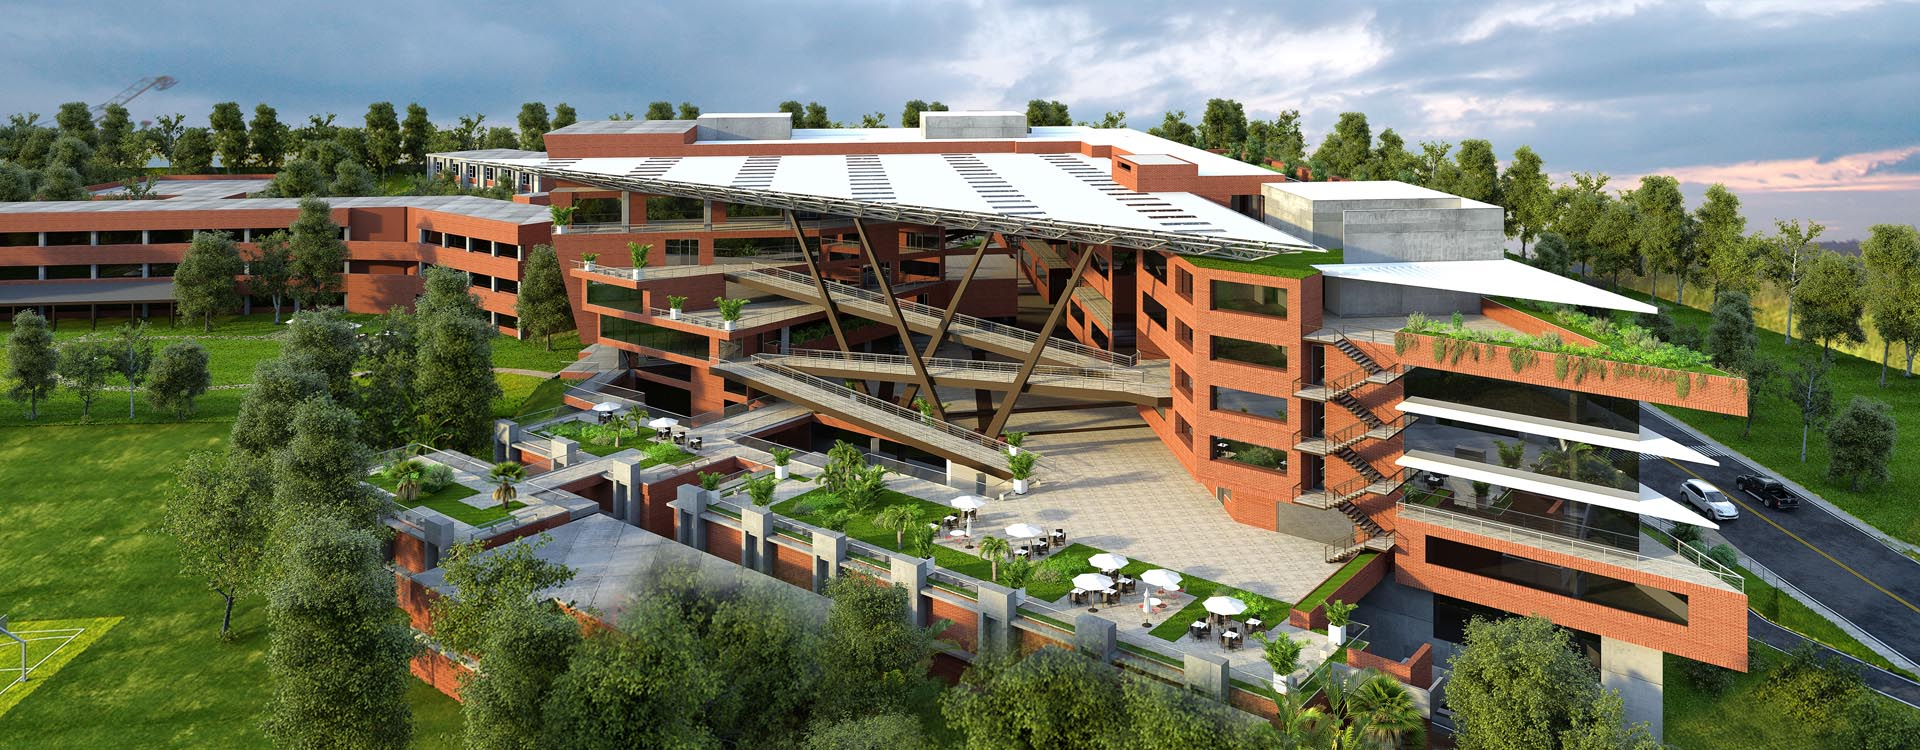
\includegraphics[height=13.25cm]{plantilla/portadacit.jpg}}
% 		\makebox[\textwidth]{
% 			\begin{overpic}[height=13.25cm]{\imagenportada}
% 				\put(63,0){
\includegraphics[height=1.15in]{plantilla/fondologo_grande.png}}
% 				\put(64.5,2){
\includegraphics[height=0.55in]{plantilla/logoUVGblanco.eps}}
% 			\end{overpic}
% 		}
% 		%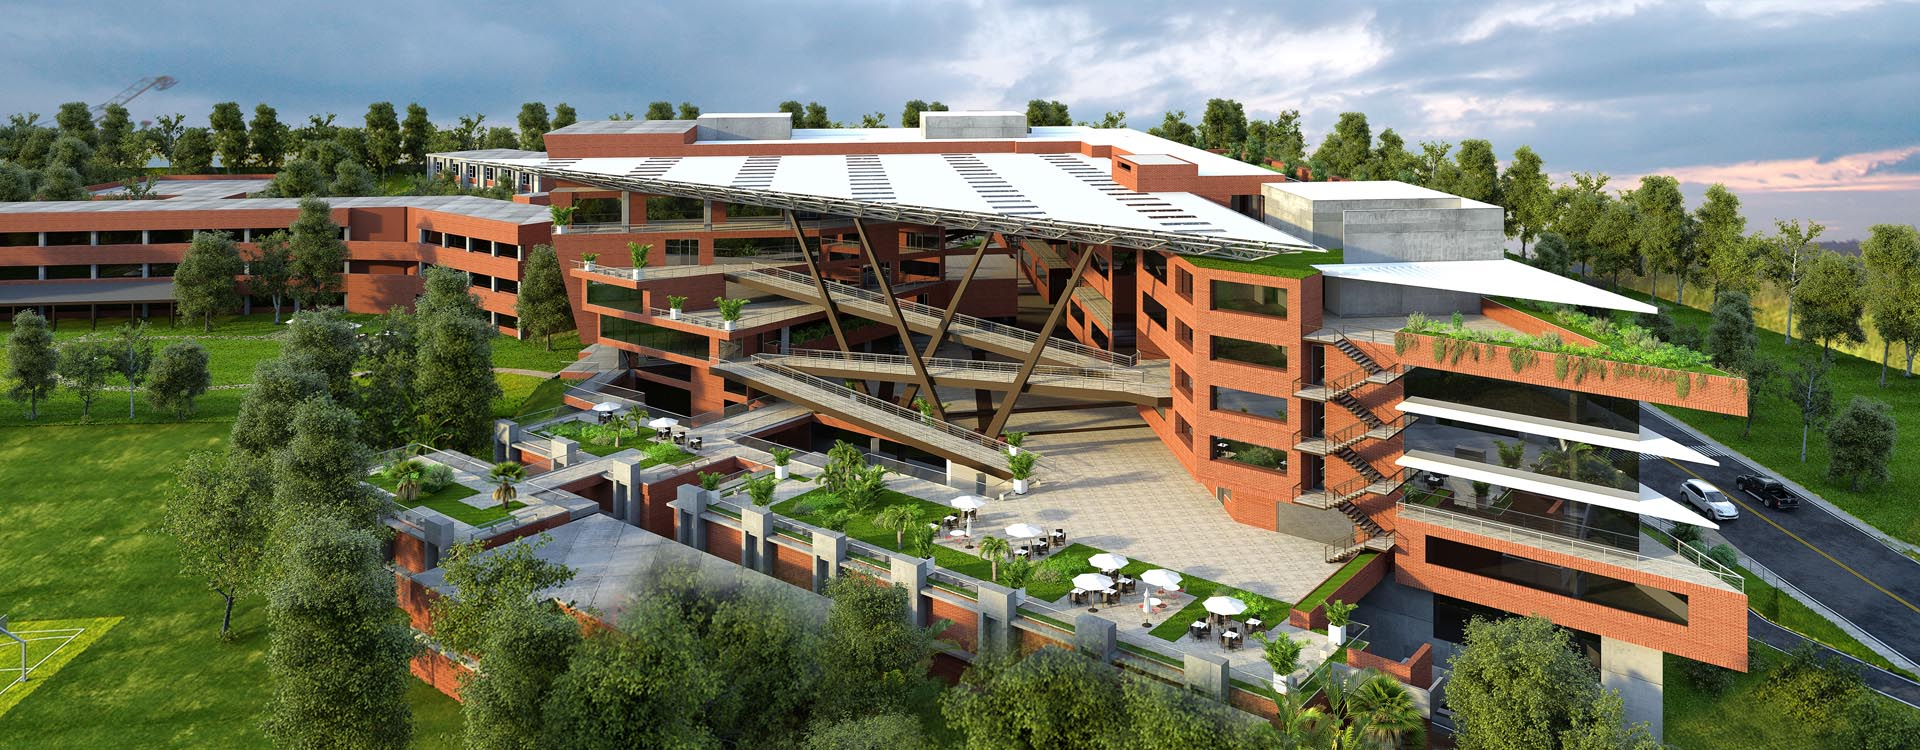
\includegraphics[height=13.25cm]{plantilla/portadacit.jpg}
% 	\end{figure}
% 	\restoregeometry
% 	\blankpage
% \fi

% ==============================================================================
% PRIMERAS PÁGINAS (Carátulas más hojas de guarda)
% ==============================================================================
\ifdefined\CAPcaratula
	\newpage
	\cleardoublepage\phantomsection
	% \pdfbookmark{Carátula}{toc}
	\pagecolor{white}
	\color{black}
	\setcounter{page}{1}
	\pagenumbering{roman}
	\thispagestyle{empty}
	\begin{center}
		\LARGE UNIVERSIDAD DEL VALLE DE GUATEMALA\\
		\LARGE Facultad de \uvgfacultad \\[0.75cm]
	\end{center}
	\begin{figure}[h]
		\begin{center}
			
\includegraphics[height=5.5 cm]{plantilla/escudoUVGnegro.eps}
			\vspace{0.5in}
		\end{center}
	\end{figure}
	\begin{center}
		% \Large \textbf{\nohyphens{\titulotesis}} \\
		\LARGE \textbf{\titulotesis} \\
		\vfill
		\Large \nohyphens{Trabajo de graduación presentado por \nombreestudiante \ para optar al grado académico de Licenciado en \uvgcarrera} \\
		\vfill
		\large Guatemala, \\
		\vspace{1em}
		\anoentrega
		\blankpage
	\end{center}

	\ifdefined\printver
		\blankpage
		\blankpage

		\newpage
		\cleardoublepage\phantomsection
		\pagecolor{white}
		\color{black}
		\setcounter{page}{1}
		\pagenumbering{roman}
		\thispagestyle{empty}
		\begin{center}
			\LARGE UNIVERSIDAD DEL VALLE DE GUATEMALA\\
			\LARGE Facultad de \uvgfacultad \\[0.75cm]
		\end{center}
		\begin{figure}[h]
			\begin{center}
				
\includegraphics[height=5.5 cm]{plantilla/escudoUVGnegro.eps}
				\vspace{0.5in}
			\end{center}
		\end{figure} 
		\begin{center}
			\Large \textbf{\nohyphens{\titulotesis}} \\
			%\LARGE \textbf{\titulotesis} \\
			\vfill
			\Large \nohyphens{Trabajo de graduación presentado por \nombreestudiante \ para optar al grado académico de Licenciado en \uvgcarrera} \\
			\vfill
			\large Guatemala, \\
			\vspace{1em}
			\anoentrega
		\end{center}
	\fi
\fi

\ifdefined\CAPcaratula
	\newpage
	\cleardoublepage\phantomsection
	% \pdfbookmark{Carátula}{toc}
	\pagecolor{white}
	\color{black}
	\setcounter{page}{1}
	\pagenumbering{roman}
	\thispagestyle{empty}
	\begin{center}
		\LARGE UNIVERSIDAD DEL VALLE DE GUATEMALA\\
		\LARGE Facultad de \uvgfacultad \\[0.75cm]
	\end{center}
	\begin{figure}[h]
		\begin{center}
			
\includegraphics[height=5.5 cm]{plantilla/escudoUVGnegro.eps}
			\vspace{0.5in}
		\end{center}
	\end{figure}
	\begin{center}
		% \Large \textbf{\nohyphens{\titulotesis}} \\
		\LARGE \textbf{\titulotesis} \\
		\vfill
		\Large \nohyphens{Trabajo de graduación presentado por \nombreestudiante \ para optar al grado académico de Licenciado en \uvgcarrera} \\
		\vfill
		\large Guatemala, \\
		\vspace{1em}
		\anoentrega
		\blankpage
	\end{center}

	\ifdefined\printver
		\blankpage
		\blankpage

		\newpage
		\cleardoublepage\phantomsection
		\pagecolor{white}
		\color{black}
		\setcounter{page}{1}
		\pagenumbering{roman}
		\thispagestyle{empty}
		\begin{center}
			\LARGE UNIVERSIDAD DEL VALLE DE GUATEMALA\\
			\LARGE Facultad de \uvgfacultad \\[0.75cm]
		\end{center}
		\begin{figure}[h]
			\begin{center}
				
\includegraphics[height=5.5 cm]{plantilla/escudoUVGnegro.eps}
				\vspace{0.5in}
			\end{center}
		\end{figure}
		\begin{center}
			\Large \textbf{\nohyphens{\titulotesis}} \\
			%\LARGE \textbf{\titulotesis} \\
			\vfill
			\Large \nohyphens{Trabajo de graduación presentado por \nombreestudiante \ para optar al grado académico de Licenciado en \uvgcarrera} \\
			\vfill
			\large Guatemala, \\
			\vspace{1em}
			\anoentrega
		\end{center}
	\fi
\fi

% ==============================================================================
% HOJA DE FIRMAS
% ==============================================================================
\ifdefined\CAPfirmas
	\newpage
	\clearchapter\phantomsection
	\thispagestyle{empty}
	\vspace*{0.5in}
	\large Vo.Bo.:\\[1cm]
	\begin{center}
		(f) \rule[1pt]{4 in}{1pt}\\
		\nombrecoordinador
	\end{center}
	\vspace{1in}

	\begin{center}
		(f) \rule[1pt]{4 in}{1pt}\\
		\nombreasesor \\[1in]
	\end{center}
	\vspace{1in}

	Fecha de aprobación: Guatemala, 18 de noviembre de \anoaprobacion.
	\normalsize
\fi

% Comentar para formato estilo libro en la numeración de páginas (NO 
% compatible con la guía UVG 2019)
\pagestyle{plain}
% ==============================================================================
% CONTENIDO DEL TRABAJO
% ==============================================================================
% PREFACIO
% ------------------------------------------------------------------------------
\ifdefined\CAPprefacio
	\newpage
	\clearchapter\phantomsection
	\chapter*{Prefacio}
	\ifdefined\parpordefecto
		\defaultparformat{a-prefacio}
	\else
		\input{a-prefacio}
	\fi
	\addcontentsline{toc}{chapter}{Prefacio}
\fi

% ÍNDICE GENERAL
% ------------------------------------------------------------------------------
\ifdefined\CAPindice
	\newpage
	\clearchapter\phantomsection
	\renewcommand{\contentsname}{Índice}
	%\phantomsection
	\pdfbookmark{\contentsname}{toc}
	%\pdfbookmark{Índice}{toc}
	\tableofcontents
\fi

% LISTADO DE FIGURAS
% ------------------------------------------------------------------------------
\ifdefined\CAPfiguras
	\newpage
	\clearchapter\phantomsection
	\renewcommand{\listfigurename}{Lista de figuras}
	\listoffigures
	\addcontentsline{toc}{chapter}{Lista de figuras}
\fi

% LISTADO DE CUADROS
% ------------------------------------------------------------------------------
\ifdefined\CAPcuadros
	\newpage
	\clearchapter\phantomsection
	\renewcommand{\listtablename}{Lista de cuadros}
	\listoftables
	\addcontentsline{toc}{chapter}{Lista de cuadros}
\fi

% RESUMEN
% ------------------------------------------------------------------------------
\ifdefined\CAPresumen
	\newpage
	\clearchapter\phantomsection
	\chapter*{Resumen}
	\ifdefined\parpordefecto
		\defaultparformat{b-resumen}
	\else
		% !TEX root = z-main.tex

El proyecto tuvo como propósito preservar digitalmente y divulgar el patrimonio cultural guatemalteco mediante el desarrollo de modelos tridimensionales del sitio arqueológico Kaminaljuyú. Este sitio, de gran relevancia histórica para el altiplano central de Guatemala, se encuentra en gran parte sepultado por la urbanización. Esta situación ha dificultado su acceso y estudio.

Para atender esta problemática, se elaboraron seis modelos tridimensionales de montículos seleccionados a partir de información arqueológica validada por especialistas. El trabajo permitió reconstruir digitalmente estructuras que no son visibles en la actualidad y preparar dichos modelos para su integración en una aplicación de realidad aumentada orientada a la educación y la difusión cultural.

Se obtuvieron representaciones tridimensionales fieles. Estas incorporaron texturas y acabados que favorecieron la comprensión de la apariencia original de los montículos. Los archivos finales se almacenaron en formatos compatibles, garantizando su preservación y posible reutilización en futuros proyectos de investigación o divulgación.

Se concluyó que la digitalización de sitios arqueológicos mediante modelado tridimensional y su aplicación en entornos de realidad aumentada constituye una estrategia eficaz para la conservación del patrimonio. Se sugiere su continuidad en otras áreas arqueológicas del país.
	\fi
	\addcontentsline{toc}{chapter}{Resumen}
\fi

% ABSTRACT
% ------------------------------------------------------------------------------
\ifdefined\CAPabstract
	\newpage
	\clearchapter\phantomsection
	\chapter*{Abstract}
	\ifdefined\parpordefecto
		\defaultparformat{c-abstract}
	\else
		% !TEX root = z-main.tex

The project aimed to digitally preserve and disseminate Guatemalan cultural heritage through the development of three-dimensional models of the archaeological site of Kaminaljuyú. This site, of great historical significance for the central highlands of Guatemala, is largely buried beneath urban development. This situation has hindered its access and study.

To address this issue, six three-dimensional models of selected mounds were created based on archaeological information validated by specialists. The work made it possible to digitally reconstruct structures that are no longer visible today and to prepare these models for integration into an augmented reality application oriented toward education and cultural dissemination.

Faithful three-dimensional representations were obtained. These incorporated textures and finishes that enhanced the understanding of the original appearance of the mounds. The final files were stored in compatible formats, ensuring their preservation and potential reuse in future research or dissemination projects.

It was concluded that the digitalization of archaeological sites through three-dimensional modeling and its application in augmented reality environments constitutes an effective strategy for heritage conservation. Its continuation is suggested in other archaeological areas of the country.
	\fi
	\addcontentsline{toc}{chapter}{Abstract}
\fi

% INTRODUCCIÓN
% ------------------------------------------------------------------------------
\ifdefined\CAPintroduccion
	\newpage
	\clearchapter
	\pagenumbering{arabic}
	\setcounter{page}{1}
	\chapter{Introducción}
	\ifdefined\parpordefecto
		\defaultparformat{d-introduccion}
	\else
		% !TEX root = z-main.tex

El avance de las tecnologías digitales transformó las formas de preservar, estudiar y difundir el patrimonio cultural. En este contexto, el modelado tridimensional (\gls{3d}), junto con la realidad aumentada (\gls{RA}), se consolidaron como herramientas fundamentales en la arqueología y la museología. Estas tecnologías permitieron recrear digitalmente sitios históricos, incluidos aquellos parcialmente desaparecidos o, como Kaminaljuyú, aún enterrados.

Kaminaljuyú, ubicado en el altiplano central guatemalteco, fue una de las ciudades más importantes del período preclásico mesoamericano. Su ocupación abarcó aproximadamente desde el año 1200 a. C. hasta el 900 d. C., extendiéndose sobre una superficie de alrededor de cinco kilómetros cuadrados y conformándose por más de 230 montículos. Debido al crecimiento urbano de la Ciudad de Guatemala, gran parte del sitio fue destruido o cubierto por construcciones modernas, conservándose únicamente cerca de cuarenta montículos, de los cuales nueve permanecen resguardados dentro del Parque Arqueológico Kaminaljuyú. Entre las estructuras más representativas que aún se mantienen visibles se encuentran la Acrópolis (C-II-4) y la Estructura E de La Palangana. Asimismo, hay estructuras que se encuentran cubiertas por la vegetación, dificultando su interpretación volumétrica. Esta pérdida progresiva del paisaje arqueológico ha planteado la necesidad de recurrir a herramientas digitales para documentar, preservar y facilitar la comprensión visual de lo que permanece del sitio.

En este marco, el trabajo tuvo como propósito modelar en \gls{3d} una selección de estructuras de Kaminaljuyú, con el fin de integrarlas en una aplicación de realidad aumentada que posibilitara su visualización e interacción digital. El desarrollo se basó en el uso del software Blender, empleando datos técnicos proporcionados por el área de arqueología, la cual validó cada modelo. La planificación del proyecto se gestionó de manera centralizada a través de la plataforma Notion, donde se documentaron los avances y se asignaron las tareas correspondientes.

El proceso incluyó la recopilación y análisis de información arqueológica, la construcción progresiva de los modelos desde las bases hasta las secciones superiores, la incorporación de texturas seleccionadas desde Poly Haven y la validación arqueológica respectiva. Los modelos finales fueron almacenados en un repositorio privado en GitHub en formatos compatibles, mientras que los archivos fuente se conservaron en OneDrive para garantizar su preservación.

La investigación demostró que el uso de herramientas digitales contribuyó a la preservación y difusión del patrimonio maya guatemalteco. Asimismo, se planteó que los resultados no se limitaron al ámbito académico o técnico, sino que también ofrecieron beneficios para instituciones culturales, turísticas y educativas interesadas en promover el conocimiento del pasado mediante experiencias tecnológicas inmersivas.

El trabajo se estructura en capítulos que abordan el contexto arqueológico, la metodología de modelado y desarrollo, los resultados obtenidos y la discusión final.

En conjunto, el trabajo evidenció que la integración de tecnologías tridimensionales y de realidad aumentada constituye una herramienta viable para la conservación digital del patrimonio arqueológico guatemalteco.
	\fi
\fi

% ANTECEDENTES
% ------------------------------------------------------------------------------
\ifdefined\CAPantecedentes
	\newpage
	\chapter{Antecedentes}
	\ifdefined\parpordefecto
		\defaultparformat{e-antecedentes}
	\else
		% !TEX root = z-main.tex

Puede encontrarse un trabajo similar en \cite{hoover2010bio} o bien \cite{park2014design}
	\fi
\fi

% JUSTIFICACIÓN
% ------------------------------------------------------------------------------
\ifdefined\CAPjustificacion
	\newpage
	\chapter{Justificación}
	\ifdefined\parpordefecto
		\defaultparformat{f-justificacion}
	\else
		% !TEX root = z-main.tex

\section{Justificación}

El modelado tridimensional de las ruinas arqueológicas de Kaminaljuyú constituye un aporte pertinente para la preservación y la divulgación del patrimonio cultural guatemalteco, al ofrecer representaciones digitales que facilitan el acceso, la interpretación y el aprendizaje sobre un sitio cuyo paisaje arqueológico ha sido sustancialmente alterado por la urbanización.

\subsection*{Dimensión patrimonial: pérdida por urbanización y acceso al patrimonio}
Durante la época prehispánica, Kaminaljuyú abarcó aproximadamente cinco kilómetros cuadrados y estuvo conformado por más de 230 montículos. Debido al crecimiento urbano de la ciudad de Guatemala, gran parte del sitio fue destruido o quedó cubierto por construcciones modernas; se estima que hoy se conservan de forma visible alrededor de cuarenta montículos, de los cuales nueve se resguardan en el Parque Arqueológico Kaminaljuyú \cite{HemerotecaPL2016}. Esta reducción del paisaje original limita la posibilidad de observación y estudio in situ, particularmente en estructuras emblemáticas como la Acrópolis (C-II-4) o sectores de La Palangana, donde la erosión y el paso del tiempo dificultan comprender sus volúmenes y relaciones espaciales. En este contexto, la reconstrucción digital aporta una ventana interpretativa que, sin sustituir el trabajo arqueológico, posibilita recuperar visualmente formas, jerarquías y disposiciones que hoy no son evidentes \cite{FundacionWiese2017}. Además, se alinea con iniciativas nacionales de digitalización de bienes culturales impulsadas por el Ministerio de Cultura y Deportes \cite{MCD2024}.

\subsection*{Dimensión educativa: aprendizaje significativo y divulgación accesible}
La integración de modelos \gls{3d} en entornos de realidad aumentada favorece procesos de aprendizaje activo, al permitir la exploración situada de estructuras y la relación entre el espacio físico y la información digital. La literatura señala que la RA incrementa la motivación y mejora la comprensión de contenidos complejos al ofrecer visualizaciones interactivas y contextuales, con efectos positivos en la retención del conocimiento \cite{Barroso2022,Sevilla2017,Handley2024}. En el ámbito universitario y museográfico, estas experiencias facilitan la enseñanza de historia y arqueología al presentar reconstrucciones creíbles, comparaciones antes/después y lecturas volumétricas del sitio; al mismo tiempo, habilitan recursos inclusivos para públicos no especializados mediante dispositivos móviles de amplio acceso. En consecuencia, el proyecto aporta materiales didácticos reutilizables para cursos, visitas guiadas y programas de mediación cultural, contribuyendo a la alfabetización patrimonial y tecnológica de estudiantes y visitantes.

\subsection*{Dimensión tecnológica: documentación 3D y RA como estrategia de preservación digital}
Desde el punto de vista técnico, el uso de Blender para modelado y texturizado, junto con la preparación de activos para su integración en \gls{RA}, promueve buenas prácticas de documentación y preservación digital (formatos interoperables, metadatos, trazabilidad de versiones). La estandarización hacia formatos orientados a tiempo real  facilita la portabilidad entre plataformas y la sostenibilidad a largo plazo de los recursos digitales. Estas prácticas se encuentran en sintonía con los lineamientos internacionales sobre preservación del patrimonio digital, que enfatizan la accesibilidad, autenticidad y continuidad de los contenidos culturales en entornos digitales \cite{UNESCO2003Charter}. En conjunto, el proyecto no solo provee visualizaciones para la difusión, sino que genera insumos técnicos que pueden integrarse en repositorios académicos o institucionales para su conservación y reutilización futura.

\subsection*{Síntesis}
La convergencia de estas tres dimensiones justifica la pertinencia del proyecto: (i) responde a la pérdida material del sitio mediante reconstrucciones verificables; (ii) habilita experiencias educativas accesibles y significativas; y (iii) establece un proceso técnico alineado con la preservación digital y la interoperabilidad, fortaleciendo el ecosistema de investigación y divulgación del patrimonio arqueológico guatemalteco.
	\fi
\fi

% OBJETIVOS
% ------------------------------------------------------------------------------
\ifdefined\CAPobjetivos
	\newpage
	\chapter{Objetivos}
	\ifdefined\parpordefecto
		\defaultparformat{g-objetivos}
	\else
		% !TEX root = z-main.tex

\section{Objetivo general}
Desarrollar modelos tridimensionales de las ruinas arqueológicas de Kaminaljuyú para su integración en entornos de realidad aumentada, mediante herramientas de modelado y animación \gls{3d}, con el fin de contribuir a la preservación digital y divulgación del patrimonio cultural guatemalteco.

\section{Objetivos específicos}
\begin{itemize}
    \item Diseñar seis modelos tridimensionales de montículos pertenecientes al sitio arqueológico Kaminaljuyú, con el propósito de representar digitalmente sus estructuras originales mediante el uso de software especializado en modelado y animación \gls{3d}.
    \item Implementar texturas en los modelos \gls{3d} para mejorar la precisión visual y la experiencia inmersiva, mediante técnicas de renderización y simulación.
    \item Evaluar la calidad y precisión de los modelos \gls{3d} en su integración con la realidad aumentada, mediante pruebas de visualización, interacción y retroalimentación de usuarios con experiencia en arqueología y tecnología.
\end{itemize}
	\fi
\fi

% ALCANCE
% ------------------------------------------------------------------------------
\ifdefined\CAPalcance
	\newpage
	\chapter{Alcance}
	\ifdefined\parpordefecto
		\defaultparformat{h-alcance}
	\else
		% !TEX root = z-main.tex

\section{Alcance del proyecto}
El proyecto abarcó el modelado de seis montículos de Kaminaljuyú en Blender 4.3.2, la preparación de materiales y texturas para visualización en tiempo real y la optimización de activos para su integración en una experiencia de realidad aumentada compatible con \gls{ARCore}. El alcance incluye: (i) reconstrucción geométrica y texturizado \gls{PBR} de las estructuras seleccionadas; (ii) exportación en formatos intercambiables (\texttt{.obj/.mtl}) con \gls{uv_mapping} preservado; (iii) pruebas funcionales de visualización e interacción en RA sobre dispositivos Android compatibles. Quedan fuera del alcance: escaneo tridimensional in situ (fotogrametría, LiDAR), animaciones avanzadas, y el desarrollo de una aplicación multiplataforma completa (iOS/ARKit), si bien los activos se dejaron preparados para conversión a \gls{gltf}/\gls{usdz}.

\section{Recursos disponibles}
El proyecto contó con los recursos necesarios para su desarrollo, incluyendo una estación de trabajo personal con capacidad para ejecutar software de modelado \gls{3d} (Blender 4.3.2), conexión a internet estable y acceso a plataformas como GitHub, OneDrive y Notion para el manejo de versiones, almacenamiento y seguimiento de tareas. Asimismo, se dispuso de la colaboración directa del departamento de arqueología y de la coordinación general del proyecto.

\section{Tiempo disponible}
El modelado se desarrolló con una programación semanal, estimándose la elaboración de un modelo tridimensional por semana, lo cual se ajustó a los plazos establecidos por el equipo. Se previó que la carga de trabajo resultara manejable dentro del calendario definido para el proyecto.

\section{Fuentes de información}
El proyecto contó con acceso a fuentes primarias proporcionadas por el departamento de arqueología, consistentes en medidas, croquis e imágenes de los montículos. Además, se consultaron fuentes secundarias como artículos académicos, sitios institucionales y documentos de divulgación arqueológica con respaldo oficial, entre ellos el Archivo General de Centroamérica (AGN), la Fundación Wiese y prensa especializada.

\section{Limitaciones del estudio}
\begin{itemize}
  \item \textbf{Captura tridimensional.} No se contó con campañas de fotogrametría, escaneo láser o LiDAR del sitio; el modelado fue \emph{manual} a partir de croquis, medidas y referencias arqueológicas validadas, lo que limita la precisión métrica absoluta en comparación con un levantamiento instrumental.
  \item \textbf{Dependencia de fuentes arqueológicas.} La geometría, proporciones y acabados respondieron a la información proporcionada por el área de arqueología. Cualquier actualización de dichas fuentes puede requerir iteraciones sobre los modelos.
  \item \textbf{Restricciones de hardware y reproducibilidad.} El desarrollo se realizó en una MacBook M1 Pro (16\,GB RAM). No se presentaron cuellos de botella críticos bajo este entorno; sin embargo, para replicación se recomienda como referencia mínima 16\,GB de RAM, almacenamiento SSD y, de ser posible, GPU con soporte moderno para shaders. Texturas de alta resolución incrementan uso de memoria y tiempos de carga.
  \item \textbf{Limitaciones de RA en móviles.} La visualización interactiva depende de dispositivos Android compatibles con \gls{ARCore}. Teléfonos no soportados o con sensores/cámaras fuera de especificación pueden presentar inestabilidad de \emph{tracking}, caídas de FPS o incompatibilidad. No se abordó la portabilidad nativa a iOS (\gls{ARKit}) dentro del cronograma.
  \item \textbf{Restricciones de software y formatos.} La versión objetivo fue Blender 4.3.2 con exportación \texttt{.obj/.mtl}. El flujo de RA exige activos optimizados (conteo poligonal moderado, número reducido de materiales, \gls{atlas_texturas} cuando aplica). 
  \item \textbf{Rendimiento y tamaño de activos.} Para asegurar usabilidad en RA móvil, se priorizó estabilidad del \emph{tracking} y tasa de cuadros sobre detalle extremo. Esto implica límites prácticos al \gls{poligonaje} y a la resolución/ cantidad de texturas, lo que puede reducir microdetalle visual respecto a un render fuera de línea.
\end{itemize}

\section{Autorización para publicar la información}
Se obtuvo autorización del equipo responsable del proyecto para difundir el material como parte del trabajo académico. Los modelos no fueron publicados de forma abierta, sino que se alojaron en repositorios privados y fueron respaldados en OneDrive, respetando el control del equipo sobre su uso.

\section{Áreas de excelencia que abarcó (Computación)}
El trabajo se enmarcó en tres áreas de excelencia del Departamento de Computación de la Universidad del Valle de Guatemala (UVG):
\begin{enumerate}
    \item \textbf{Ingeniería de software}: por la gestión sistemática del desarrollo de modelos digitales, el control de versiones, la documentación en Notion y el uso de herramientas colaborativas como GitHub.
    \item \textbf{Visualización de datos e interfaces gráficas}: al crear representaciones tridimensionales con fines de divulgación, educación y exploración virtual del patrimonio.
    \item \textbf{Tecnologías emergentes}: mediante la aplicación del modelado \gls{3d} y su integración en plataformas de realidad aumentada como \gls{ARCore}, en concordancia con las tendencias actuales de digitalización del patrimonio.
\end{enumerate}
	\fi
\fi

% MARCO TEÓRICO
% ------------------------------------------------------------------------------
\ifdefined\CAPmarcoteorico
	\newpage
	\chapter{Marco teórico}
	\ifdefined\parpordefecto
		\defaultparformat{i-marco_teorico}
	\else
		% !TEX root = z-main.tex

Modelado 3D: fundamentos y aplicaciones

El modelado 3D se definió como una técnica de creación digital que permitió construir representaciones tridimensionales de objetos, espacios o personajes mediante herramientas computacionales. Fue considerado una forma de escultura digital, en la cual se partía de formas básicas —como cubos, planos o esferas— y se añadía geometría para generar volumen y detalle \cite{Teijeiro2023}. Este proceso combinó aspectos técnicos y artísticos, pues requirió tanto del dominio de programas especializados como de la comprensión de la forma, el espacio y los elementos visuales.

Las aplicaciones del modelado 3D abarcaron múltiples sectores, entre ellos el cine, los videojuegos, la arquitectura, el diseño industrial y, de forma creciente, la museología y la arqueología. En este último ámbito, los modelos tridimensionales facilitaron la reconstrucción de estructuras antiguas con precisión, favoreciendo su estudio y preservación, especialmente cuando los restos físicos se encontraron fragmentados, deteriorados o, como en el caso de Kaminaljuyú, permanecieron ocultos bajo la urbanización contemporánea. Dichas reconstrucciones se integraron además en entornos de realidad aumentada, ofreciendo experiencias inmersivas independientes del estado físico del sitio.

Realidad aumentada como herramienta educativa y cultural

La realidad aumentada (RA) se describió como una tecnología que permitió superponer elementos digitales —modelos tridimensionales, imágenes, textos o sonidos— sobre la percepción del mundo real en tiempo real. A diferencia de la realidad virtual, que construyó un entorno completamente simulado, la RA combinó el espacio físico con información digital interactiva, enriqueciendo la experiencia del usuario sin aislarlo de su contexto \cite{Torres2013}.

En el ámbito artístico-cultural, la RA abrió nuevas posibilidades para la presentación, interpretación y difusión del patrimonio. Museos y centros de interpretación la adoptaron como parte de sus estrategias museográficas, posibilitando el acceso a información ampliada sobre objetos culturales, la simulación de entornos históricos y la visualización de reconstrucciones virtuales de elementos desaparecidos o dañados. Estas aplicaciones fortalecieron la accesibilidad y la comprensión del contenido expuesto \cite{Torres2013}.

Desde la educación, la RA demostró ser una herramienta eficaz. Su incorporación en procesos de enseñanza-aprendizaje promovió la participación activa, el aprendizaje experiencial y la comprensión de conceptos complejos mediante la interacción directa con representaciones visuales y tridimensionales. Investigaciones recientes evidenciaron que la RA incrementó la motivación del estudiante, mejoró la retención del conocimiento y favoreció el aprendizaje significativo, especialmente en contextos donde los contenidos resultaron difíciles de representar de manera tradicional \cite{Barroso2022,Sevilla2017}.
	\fi
\fi

% METODOLOGÍA
% ------------------------------------------------------------------------------
\ifdefined\CAPmetodologia
	\newpage
	\chapter{Metodología}
	\ifdefined\parpordefecto
		\defaultparformat{j-metodologia}
	\else
		% !TEX root = z-main.tex

\section{Enfoque metodológico}
La investigación respondió a un enfoque aplicado, con características proyectivas, descriptivas y cualitativas, orientado al desarrollo de modelos tridimensionales de estructuras arqueológicas del sitio Kaminaljuyú. El proyecto buscó representar digitalmente estos elementos mediante técnicas de modelado \gls{3d}, basadas en datos arqueológicos previamente verificados y validados por profesionales en el área, sin manipulación de variables cuantitativas. Se trató de una investigación enfocada en la reconstrucción visual y contextual de un sitio patrimonial con fines educativos, culturales y tecnológicos.

El desarrollo se realizó en un entorno interdisciplinario que integró conocimientos de arqueología, diseño digital y tecnologías de visualización. La planificación y el seguimiento de las actividades se gestionaron por medio de una plataforma digital colaborativa, la cual permitió asignar tareas semanales, validar avances y centralizar la documentación del proceso.

La planificación y el seguimiento del proyecto se gestionaron mediante una plataforma digital colaborativa, Notion, donde el equipo encargado de la gestión asignó semanalmente las tareas de modelado, organizó las prioridades y centralizó los avances. Esta plataforma permitió documentar el flujo de trabajo, dar seguimiento individual al progreso de las tareas y garantizar una trazabilidad clara del proceso. El modelado de los montículos se basó en información técnica proporcionada por especialistas en arqueología, quienes entregaron croquis, medidas e imágenes de referencia que posibilitaron representar las estructuras con fidelidad.

Una vez recibida la información, se configuró el entorno de trabajo en el software de modelado Blender, donde se establecieron las escalas apropiadas y se organizaron carpetas por montículo. La construcción tridimensional de las estructuras se inició desde las bases y avanzó progresivamente hacia las secciones superiores. Se emplearon técnicas mixtas de modelado de caja, y se previó un ritmo de producción de aproximadamente un modelo por semana, ajustado a la complejidad de cada estructura y a la retroalimentación técnica y arqueológica recibida.

Las texturas y materiales utilizados en los modelos fueron seleccionados desde el repositorio de recursos digitales Poly Haven y se aplicaron bajo la supervisión del área de arqueología, garantizando coherencia visual y contextual con los materiales históricos originales, como el barro, la piedra y los techados vegetales. Se prestó especial atención a la correcta proyección UV, evitando estiramientos o errores de mapeo en las texturas aplicadas. Cada modelo completado fue validado por especialistas arqueológicos, quienes emitieron observaciones sobre proporciones, formas y texturas. En función de estas observaciones, se realizaron los ajustes necesarios para asegurar la fidelidad de las representaciones.

Como parte del proceso de mejora técnica, se previó una participación en la comunidad oficial de Blender. Se estableció contacto con expertos para solicitar retroalimentación sobre aspectos clave del modelado. Las preguntas que se realizaron incluyeron si la topología del modelo era adecuada para su uso en realidad aumentada, si las proporciones y la escala estaban correctamente definidas dentro del espacio tridimensional, y si las texturas habían sido aplicadas sin errores visibles de mapeo UV. Se esperó que la comunidad respondiera con recomendaciones puntuales y videos explicativos, los cuales fueron analizados y aplicados para mejorar los estándares técnicos del trabajo. Esta etapa complementó la validación arqueológica, fortaleciendo la solidez técnica de los modelos que se generaron.

Los modelos finalizados fueron almacenados en un repositorio privado en GitHub, en formatos .obj y .mtl, preparados para su integración posterior. Los archivos fuente en formato .blend se conservaron localmente y estuvieron respaldados automáticamente en la nube mediante OneDrive, garantizando así la seguridad y la integridad del material original. Todo el proceso fue documentado gráficamente mediante capturas de pantalla y registros de validación, centralizados en Notion y WhatsApp.

Aunque la integración de los modelos tridimensionales en la aplicación de realidad aumentada no formó parte directa de las tareas del área de modelado, se tuvo prevista la participación en dicha fase. Esta colaboración permitió verificar el comportamiento de los modelos en el entorno digital, identificar posibles ajustes estructurales o visuales y asegurar la compatibilidad técnica con motores gráficos como \gls{ARCore}.

El análisis de los modelos se llevó a cabo mediante un proceso de validación técnica y visual, sustentado en la retroalimentación de profesionales en arqueología, quienes evaluaron aspectos como proporción, escala y coherencia estética. Desde una perspectiva técnica, se revisó la topología, el mapeo de texturas y la compatibilidad con entornos digitales. Este análisis fue de tipo cualitativo, iterativo y no estadístico, dado que se orientó a la mejora continua de los modelos a través de observación crítica y ajuste progresivo.

Finalmente, se observaron consideraciones éticas relacionadas con la representación y difusión del patrimonio cultural. Este proyecto no implicó la recolección de datos personales ni el involucramiento de individuos o comunidades. Sin embargo, se asumió el compromiso de representar con precisión los elementos arqueológicos modelados, evitando distorsiones que pudieran inducir a errores históricos o técnicos. Se mantuvo una actitud de respeto hacia la memoria cultural del pueblo maya, utilizando las tecnologías digitales con fines educativos, académicos y de conservación.

\section{Etapas de desarrollo}
\subsection{Planificación y asignación de tareas}
La gestión del proyecto se llevó a cabo a través de la plataforma Notion, en la cual el equipo responsable de la coordinación general asignó semanalmente las tareas correspondientes a cada fase del modelado. Cada semana se estableció la elaboración de un montículo específico, en función de la disponibilidad de los datos técnicos proporcionados por el área de arqueología. El avance de cada actividad quedó documentado en dicha plataforma, lo que permitió su trazabilidad y el control de entregas.

\subsection{Recolección y análisis de información arqueológica}
El equipo arqueológico especializado proporcionó las medidas, croquis e imágenes de referencia necesarios para modelar cada una de las estructuras seleccionadas. Esta información fue analizada e interpretada para ser adaptada al entorno digital, asegurando la fidelidad estructural y contextual de los modelos.

\subsection{Configuración del entorno de trabajo en Blender}
Se utilizó el software Blender, versión 4.3.2, como herramienta principal para el modelado tridimensional. Se crearon entornos de trabajo independientes para cada estructura, organizados en carpetas con nombres específicos por montículo. Se verificó la escala general del espacio tridimensional con base en los datos arqueológicos recibidos, garantizando la coherencia entre los modelos digitales y las dimensiones reales.

\subsection{Modelado tridimensional de estructuras}
El proceso de construcción de los modelos se inició desde las bases estructurales hasta los niveles superiores, respetando las proporciones y características definidas en los registros arqueológicos. El ritmo de trabajo estimado fue de un modelo por semana, dependiendo de la complejidad de cada montículo y con una semana adicional destinada a la retroalimentación obtenida tras cada revisión.

\subsection{Aplicación de texturas}
Las texturas fueron seleccionadas desde el repositorio libre Poly Haven (https://polyhaven.com), con el acompañamiento del equipo arqueológico para asegurar coherencia con los materiales originales utilizados históricamente (barro, piedra, techados vegetales, entre otros). Se revisó la correcta proyección de las texturas para evitar estiramientos o distorsiones, realizando los ajustes necesarios cuando fue requerido.

\subsection{Validación arquelógica y ajustes}
Cada modelo finalizado fue enviado al equipo especializado en arqueología para su revisión técnica y contextual. Las observaciones emitidas fueron documentadas y, en caso de ser necesario, se implementaron los ajustes técnicos correspondientes en el diseño tridimensional.

\subsection{Asesoramiento técnico externo}
Durante el desarrollo del proyecto, se previó la participación en la comunidad oficial de Blender, donde se consultaron dudas específicas relacionadas con herramientas o procesos técnicos de modelado. Estas interacciones permitieron optimizar el flujo de trabajo y mejorar la calidad de los modelos generados.

\subsection{Evaluar la calidad y precisión del modelado 3d en su integración con la aplicación de realidad aumentada}
Se llevó a cabo la evaluación de la integración de los modelos \gls{3d} en la aplicación de realidad aumentada, verificando su precisión, calidad visual y comportamiento interactivo, e incorporando la retroalimentación de usuarios especializados en arqueología y tecnología para garantizar su fidelidad y compatibilidad técnica.

\subsection{Registro}
Durante todo el desarrollo se generó documentación gráfica mediante capturas de pantalla, así como versiones intermedias y finales de cada modelo compartidas por medio de WhatsApp. Las observaciones técnicas también fueron archivadas. Los archivos finales en formato .obj y .mtl fueron subidos a un repositorio privado en GitHub con fines de respaldo y distribución técnica. Los archivos fuente en formato .blend fueron almacenados localmente y respaldados de forma automática en la nube (OneDrive), evitando así pérdidas o ediciones no autorizadas.

	\fi
\fi

% RESULTADOS
% ------------------------------------------------------------------------------
\ifdefined\CAPresultados
	\newpage
	\chapter{Resultados}
	\ifdefined\parpordefecto
		\defaultparformat{k-resultados}
	\else
		% k-resultados.tex
% !TEX root = z-main.tex

\section{Resultados}

% En esta sección se presentan los modelos tridimensionales de los montículos analizados.
% Cada subsección incluye el panel de vistas generado (malla, sólido y texturizado).


\FloatBarrier
\subsection{Montículo 3}


\begin{figure}[!htbp]
    \centering
    \caption{Montículo 3, panel de vistas}
    \label{fig:m3-panel}
    % ----- Fila 1 -----
    \begin{subfigure}{0.48\textwidth}
        \centering
        \caption{Vista en malla (wireframe)}
        \label{fig:m3-wire}
        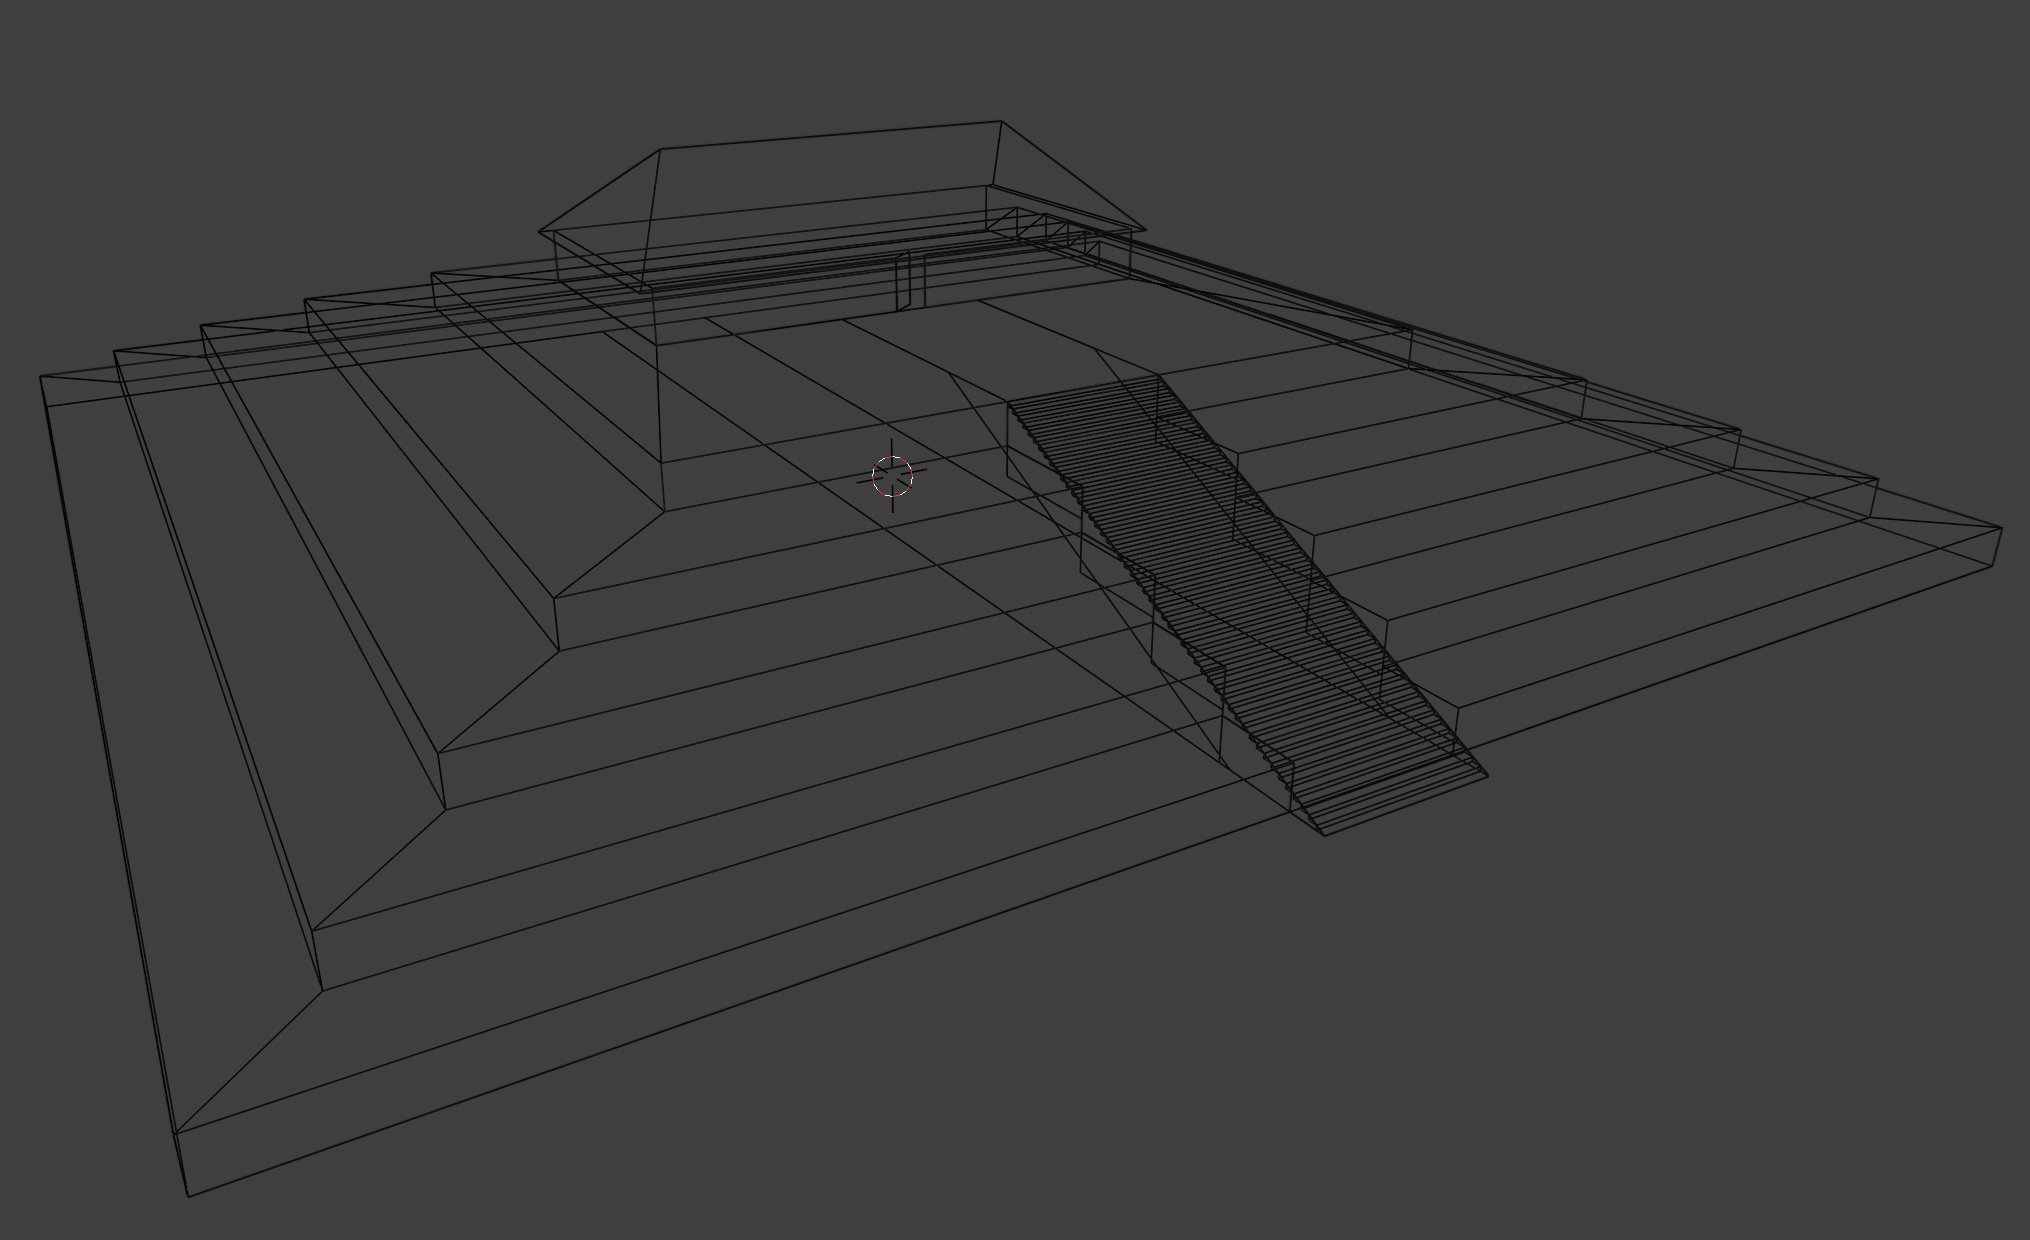
\includegraphics[width=\linewidth]{resultados/figures/m3/m3_wireframe.png}
    \end{subfigure}\hfill
    \begin{subfigure}{0.48\textwidth}
        \centering
        \caption{Vista sólida sin texturas}
        \label{fig:m3-solid}
        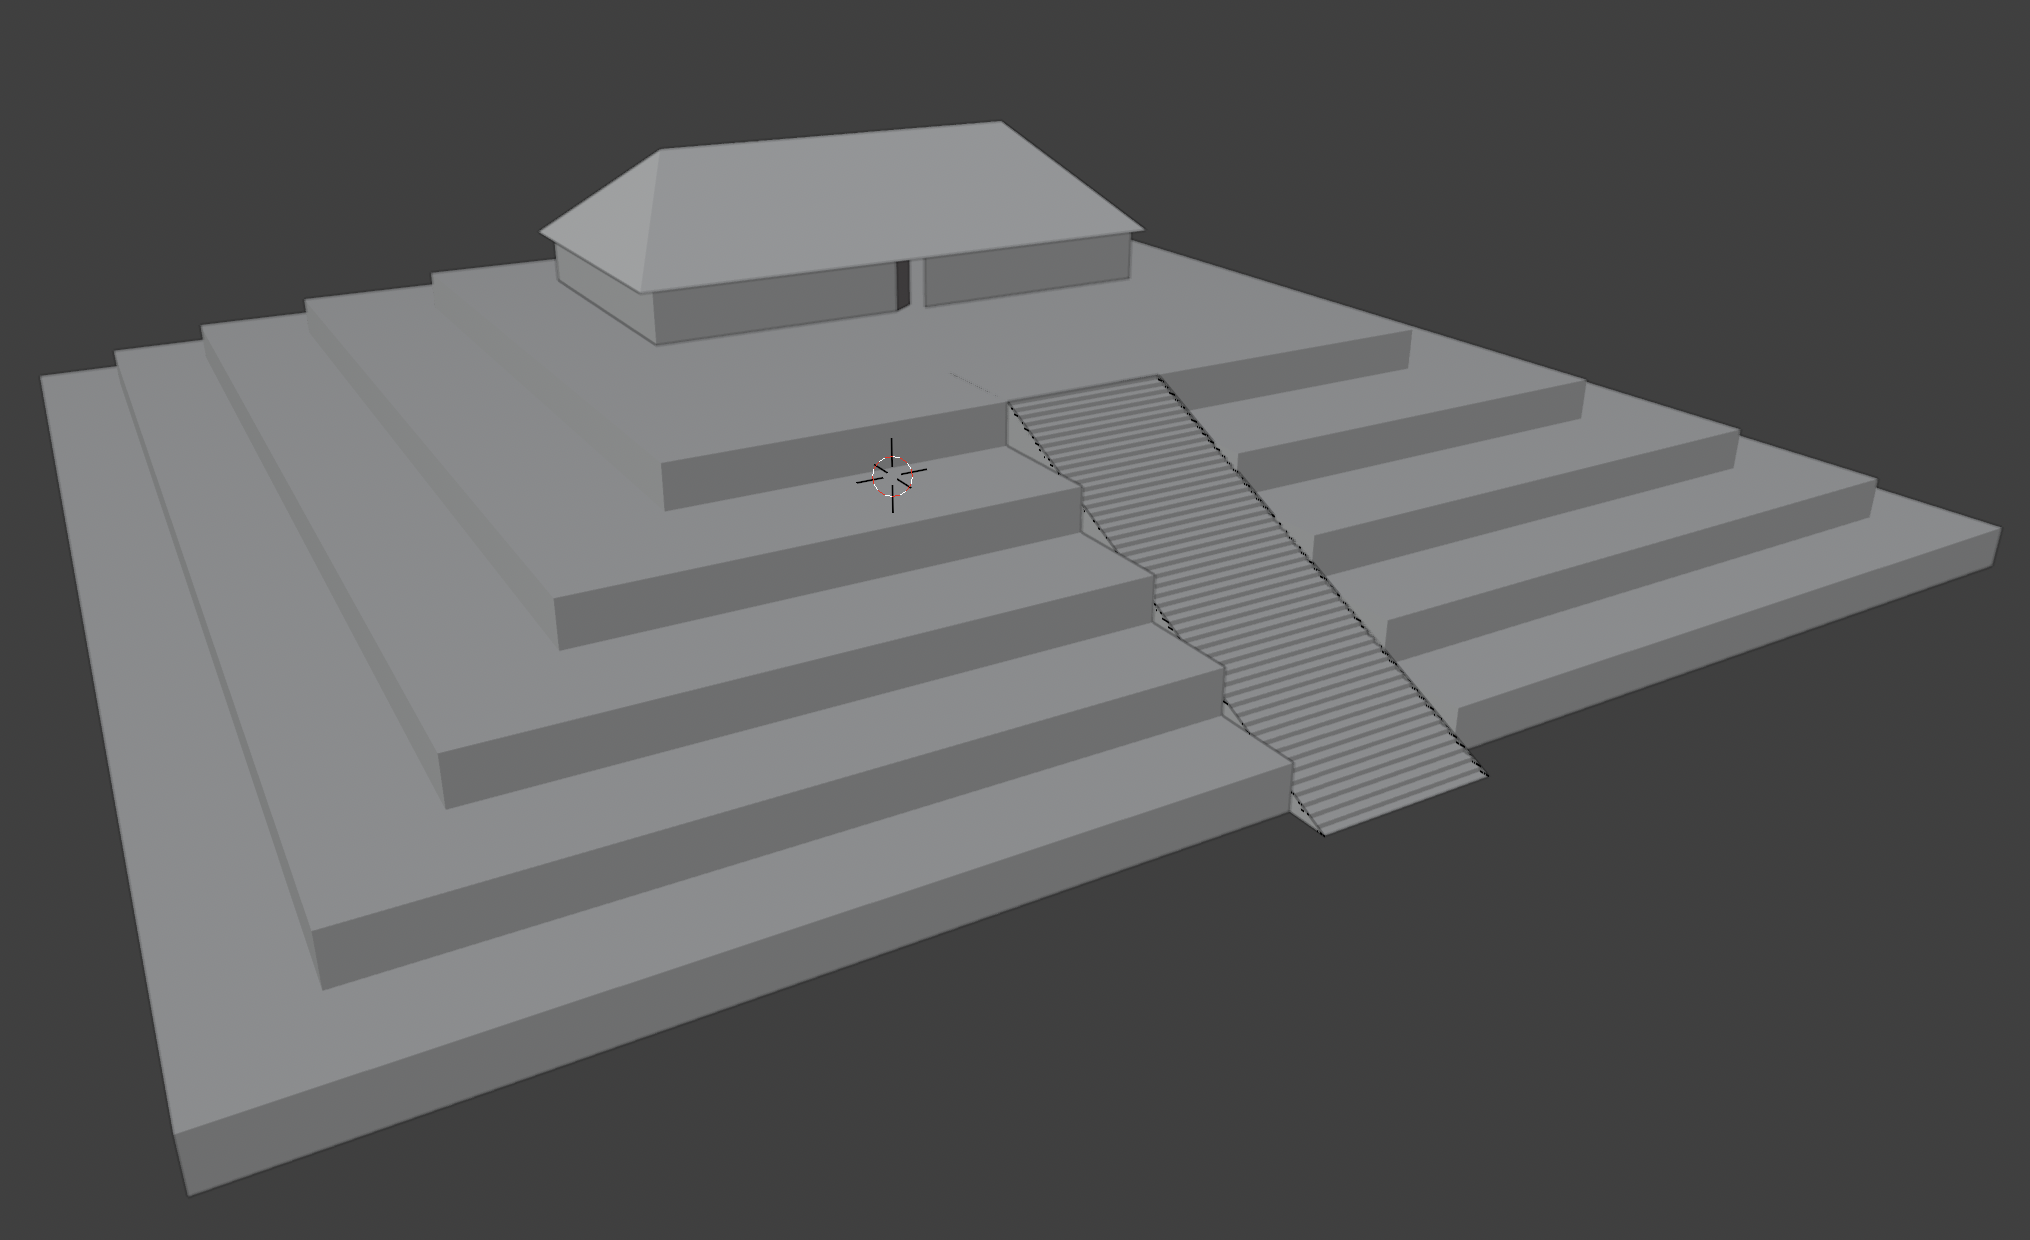
\includegraphics[width=\linewidth]{resultados/figures/m3/m3_solid.png}
    \end{subfigure}

    \vspace{0.6em}

    % ----- Fila 2 -----
    \begin{subfigure}{0.48\textwidth}
        \centering
        \caption{Vista con materiales/texturas}
        \label{fig:m3-textured}
        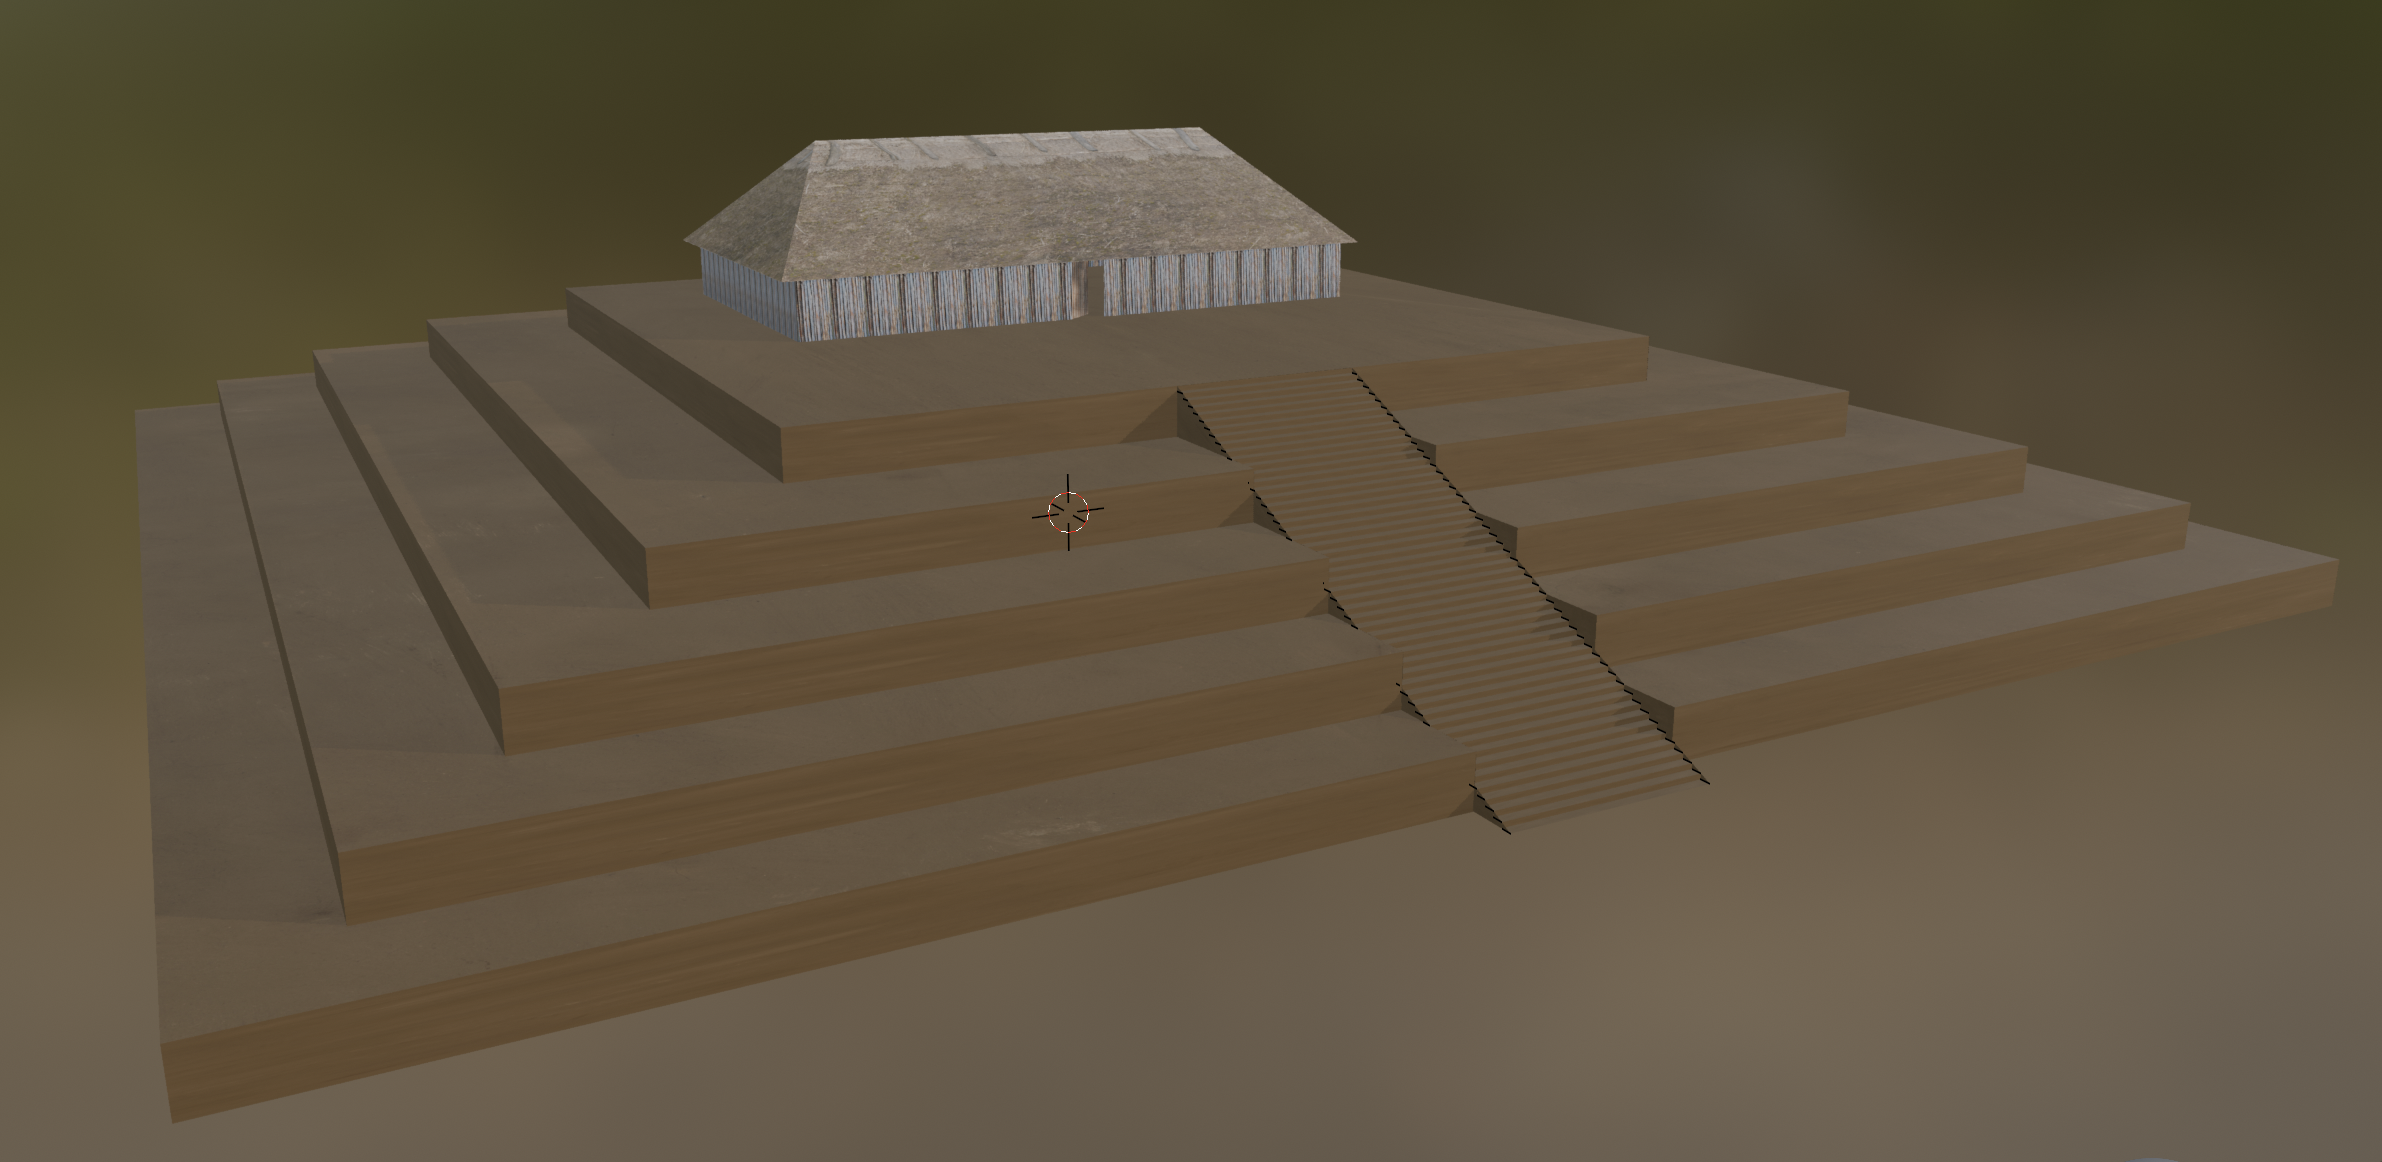
\includegraphics[width=\linewidth]{resultados/figures/m3/m3_textured_viewport.png}
    \end{subfigure}
\end{figure}
\FloatBarrier

\begin{figure}[!htbp]
    \centering
    \caption{Montículo 3 visualizado en la aplicación de realidad aumentada, mostrando la reconstrucción superpuesta en el entorno real del parque arqueológico}
    \label{fig:m3-ar}
    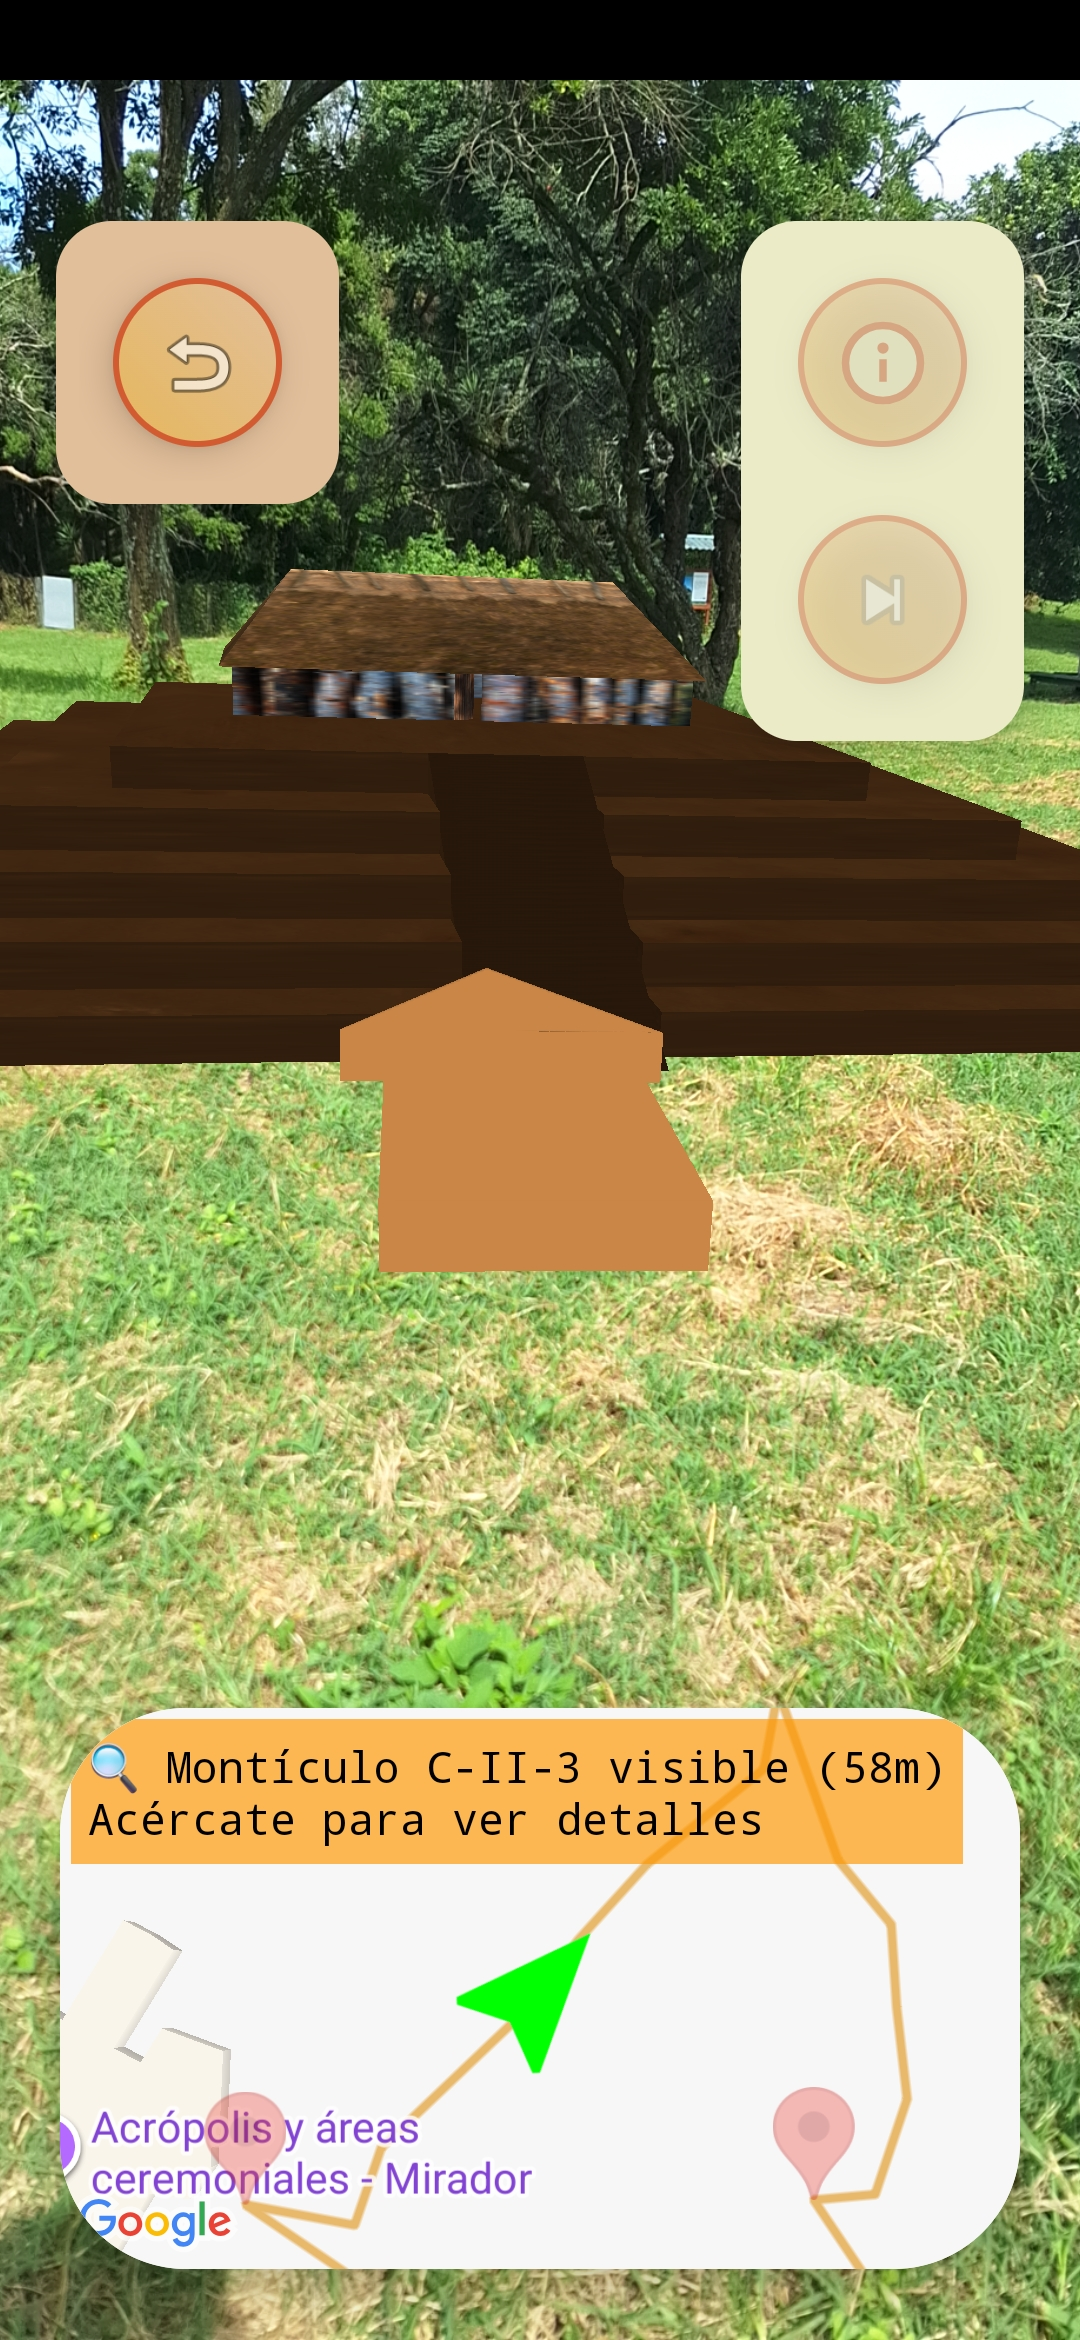
\includegraphics[width=0.48\linewidth]{resultados/figures/m3/m3_ar.jpg}
\end{figure}
\clearpage
\FloatBarrier
\subsection{Montículo 7}

\begin{figure}[!htbp]
    \centering
    \caption{Montículo 7, panel de vistas}
    \label{fig:m7-panel}
    % ----- Fila 1 -----
    \begin{subfigure}{0.48\textwidth}
        \centering
        \caption{Vista en malla (wireframe)}
        \label{fig:m7-wire}
        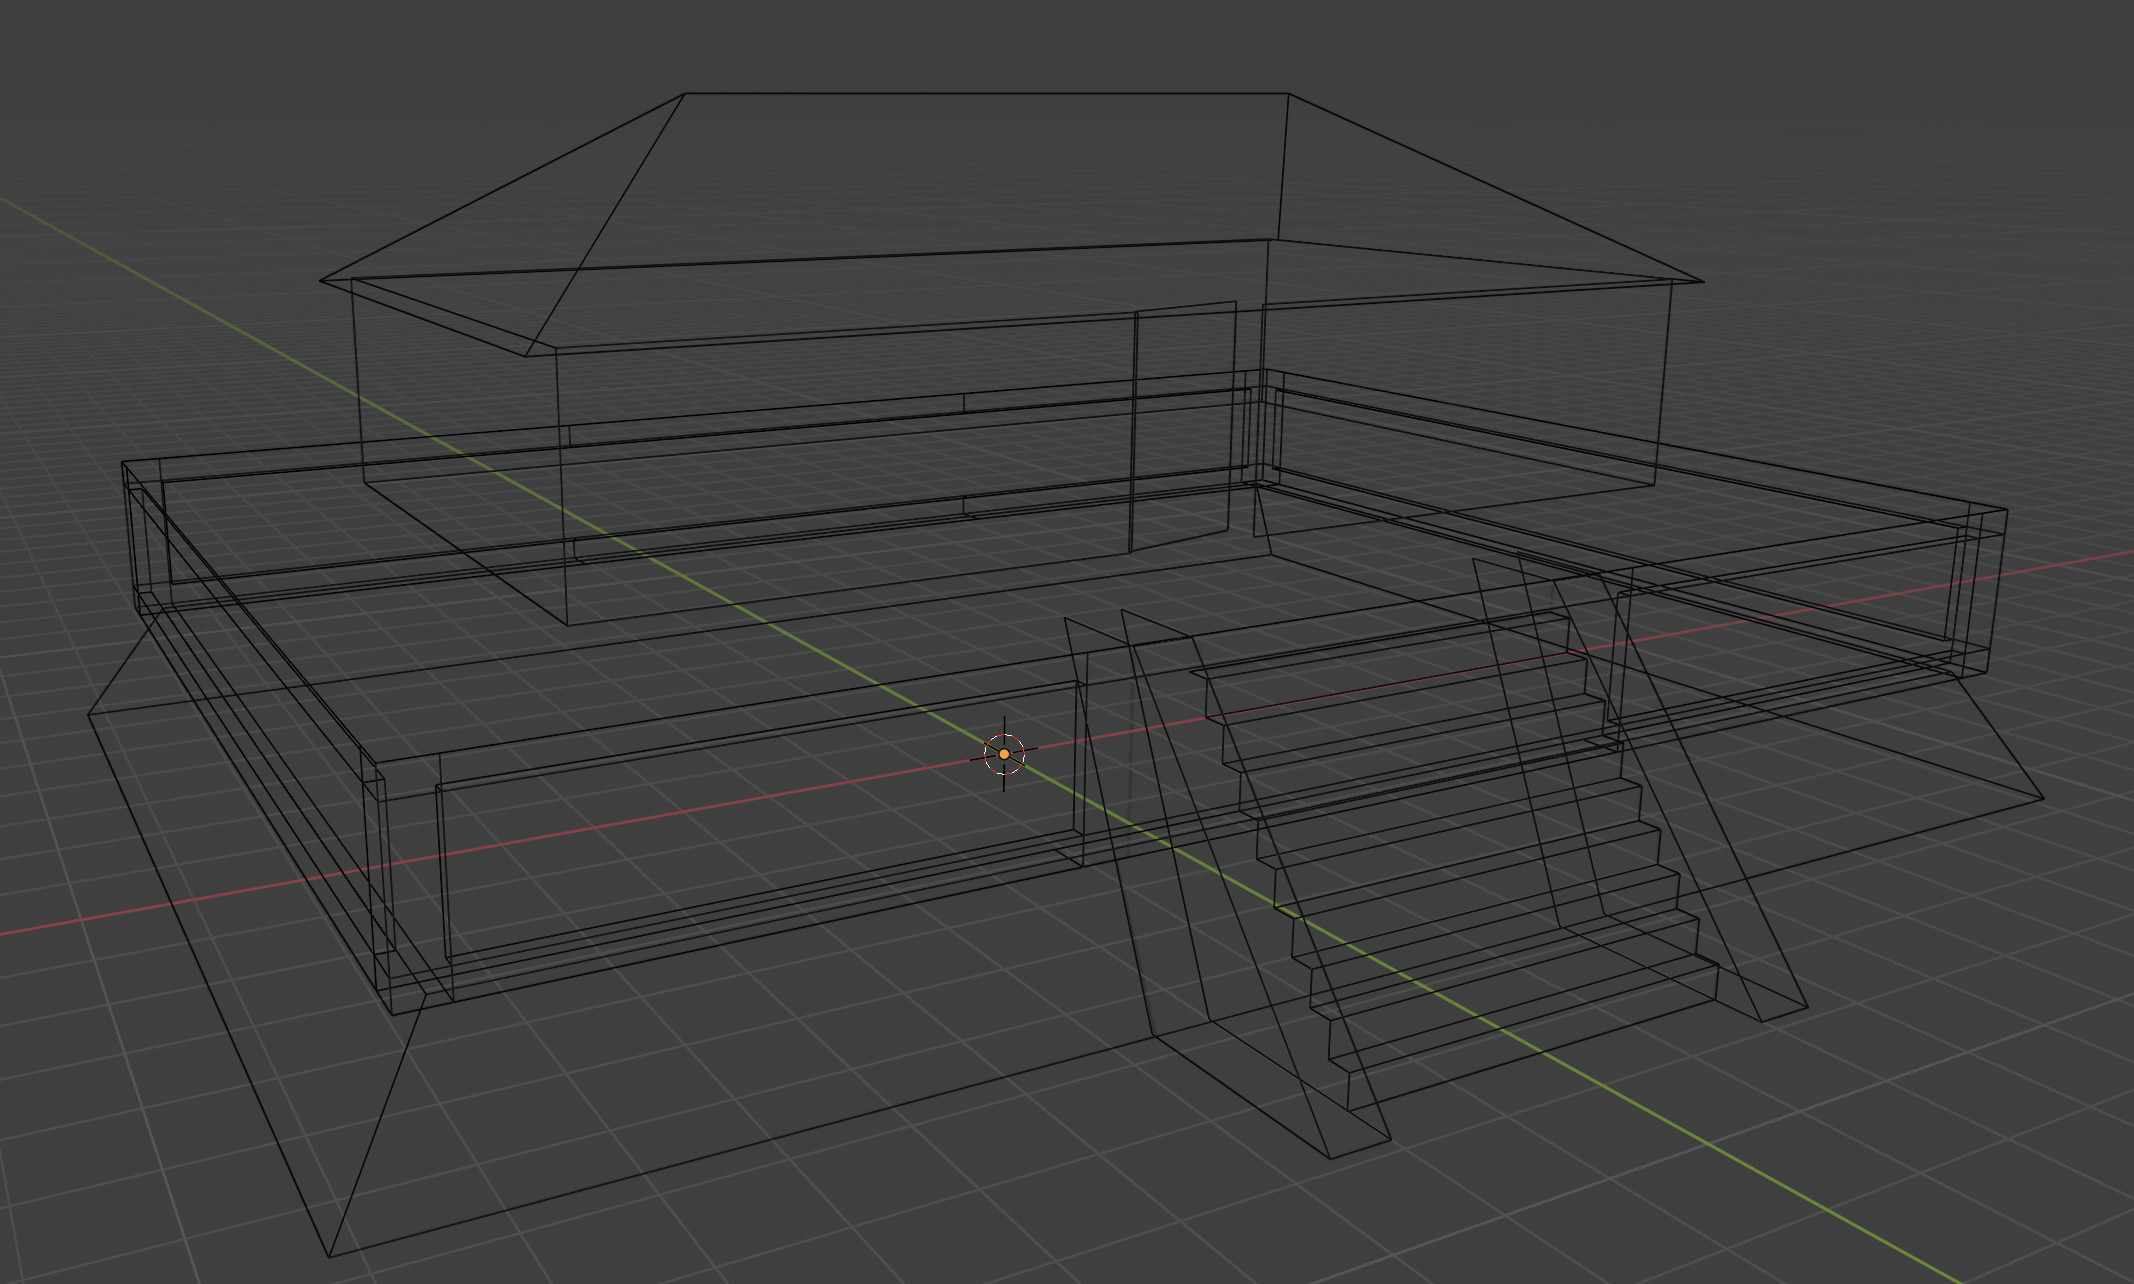
\includegraphics[width=0.85\linewidth]{resultados/figures/m7/m7_wireframe.png}
    \end{subfigure}\hfill
    \begin{subfigure}{0.48\textwidth}
        \centering
        \caption{Vista sólida sin texturas}
        \label{fig:m7-solid}
        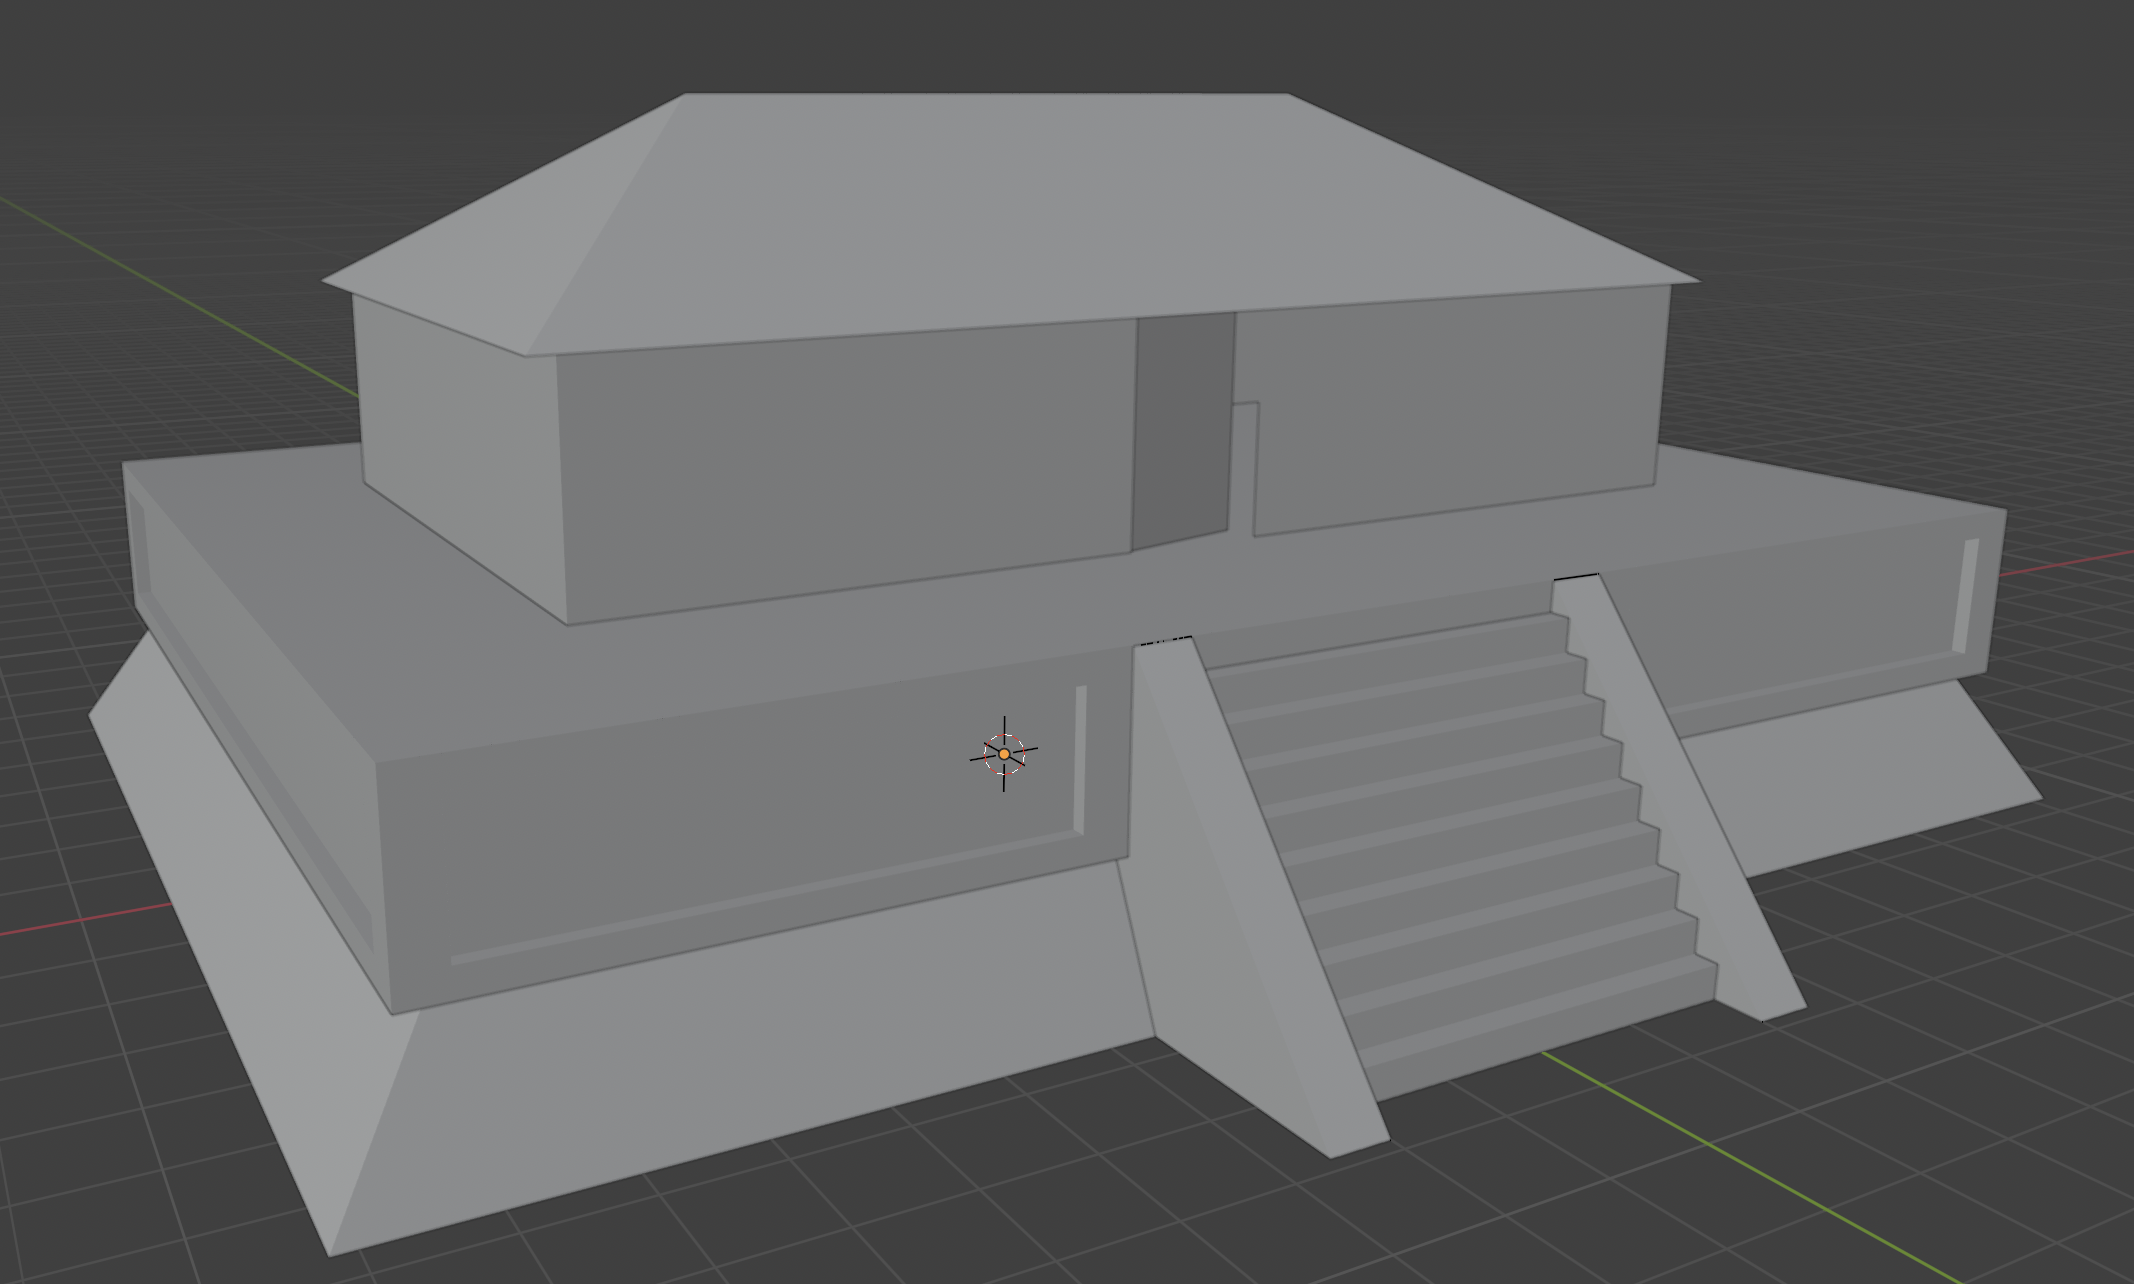
\includegraphics[width=0.85\linewidth]{resultados/figures/m7/m7_solid.png}
    \end{subfigure}

    \vspace{0.1em}

    % ----- Fila 2 -----
    \begin{subfigure}{0.48\textwidth}
        \centering
        \caption{Vista con materiales/texturas}
        \label{fig:m7-textured}
        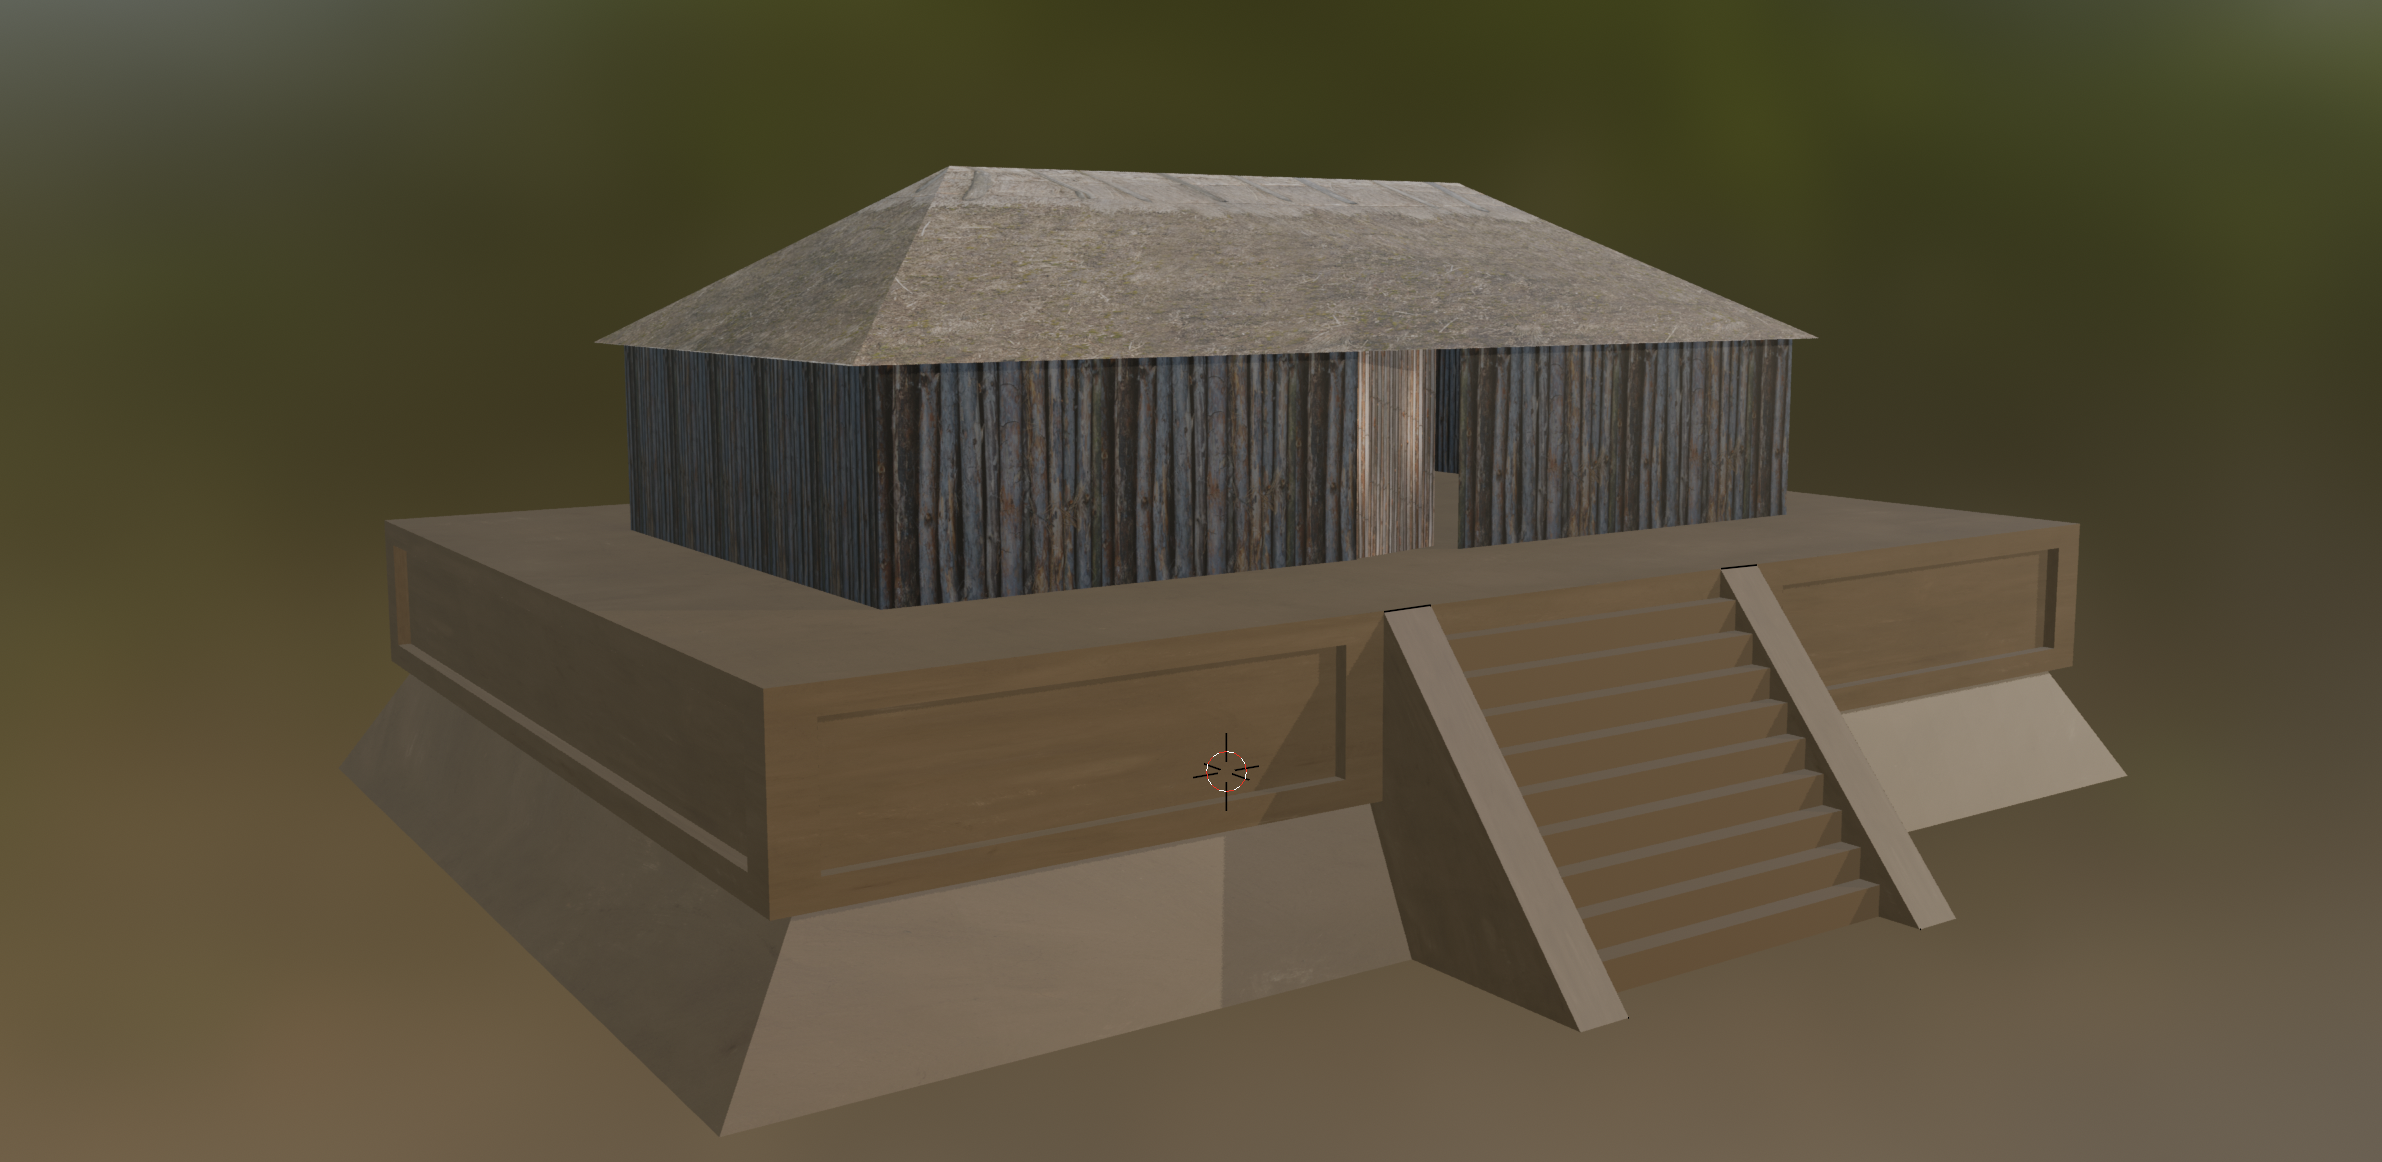
\includegraphics[width=0.85\linewidth]{resultados/figures/m7/m7_textured_viewport.png}
    \end{subfigure}
\end{figure}


\begin{figure}[!htbp]
    \centering
    \caption{Montículo 7 visualizado en la aplicación de realidad aumentada, mostrando la reconstrucción superpuesta en el entorno real del parque arqueológico}
    \label{fig:m7-ar}
    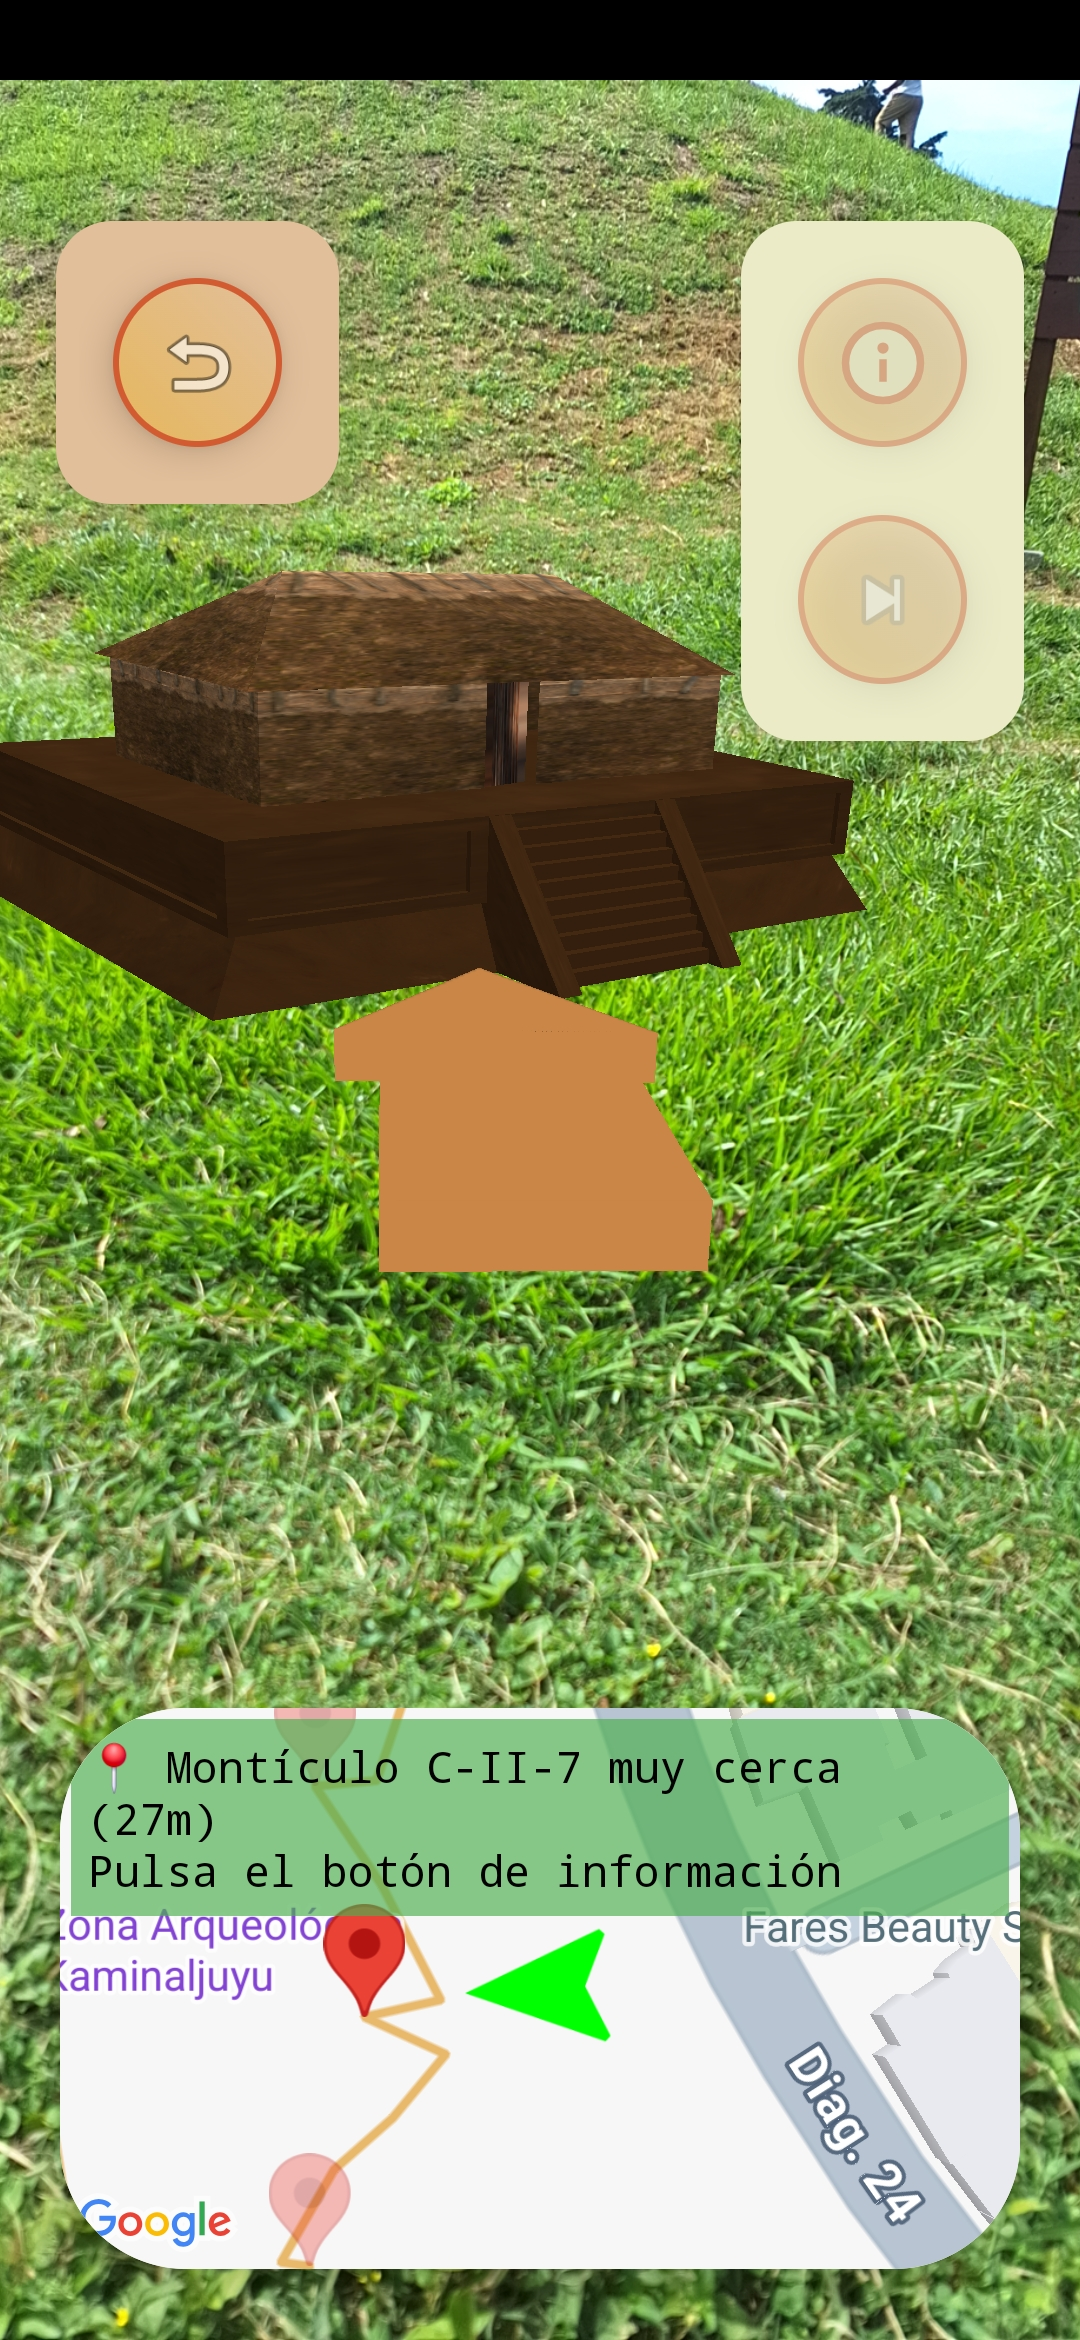
\includegraphics[width=0.28\linewidth]{resultados/figures/m7/m7_ar.jpg}
\end{figure}
\FloatBarrier
\clearpage
\FloatBarrier
\subsection{Montículo 12}

\begin{figure}[!htbp]
    \centering
    \caption{Montículo 12, panel de vistas}
    \label{fig:m12-panel}
    % ----- Fila 1 -----
    \begin{subfigure}{0.48\textwidth}
        \centering
        \caption{Vista en malla (wireframe)}
        \label{fig:m12-wire}
        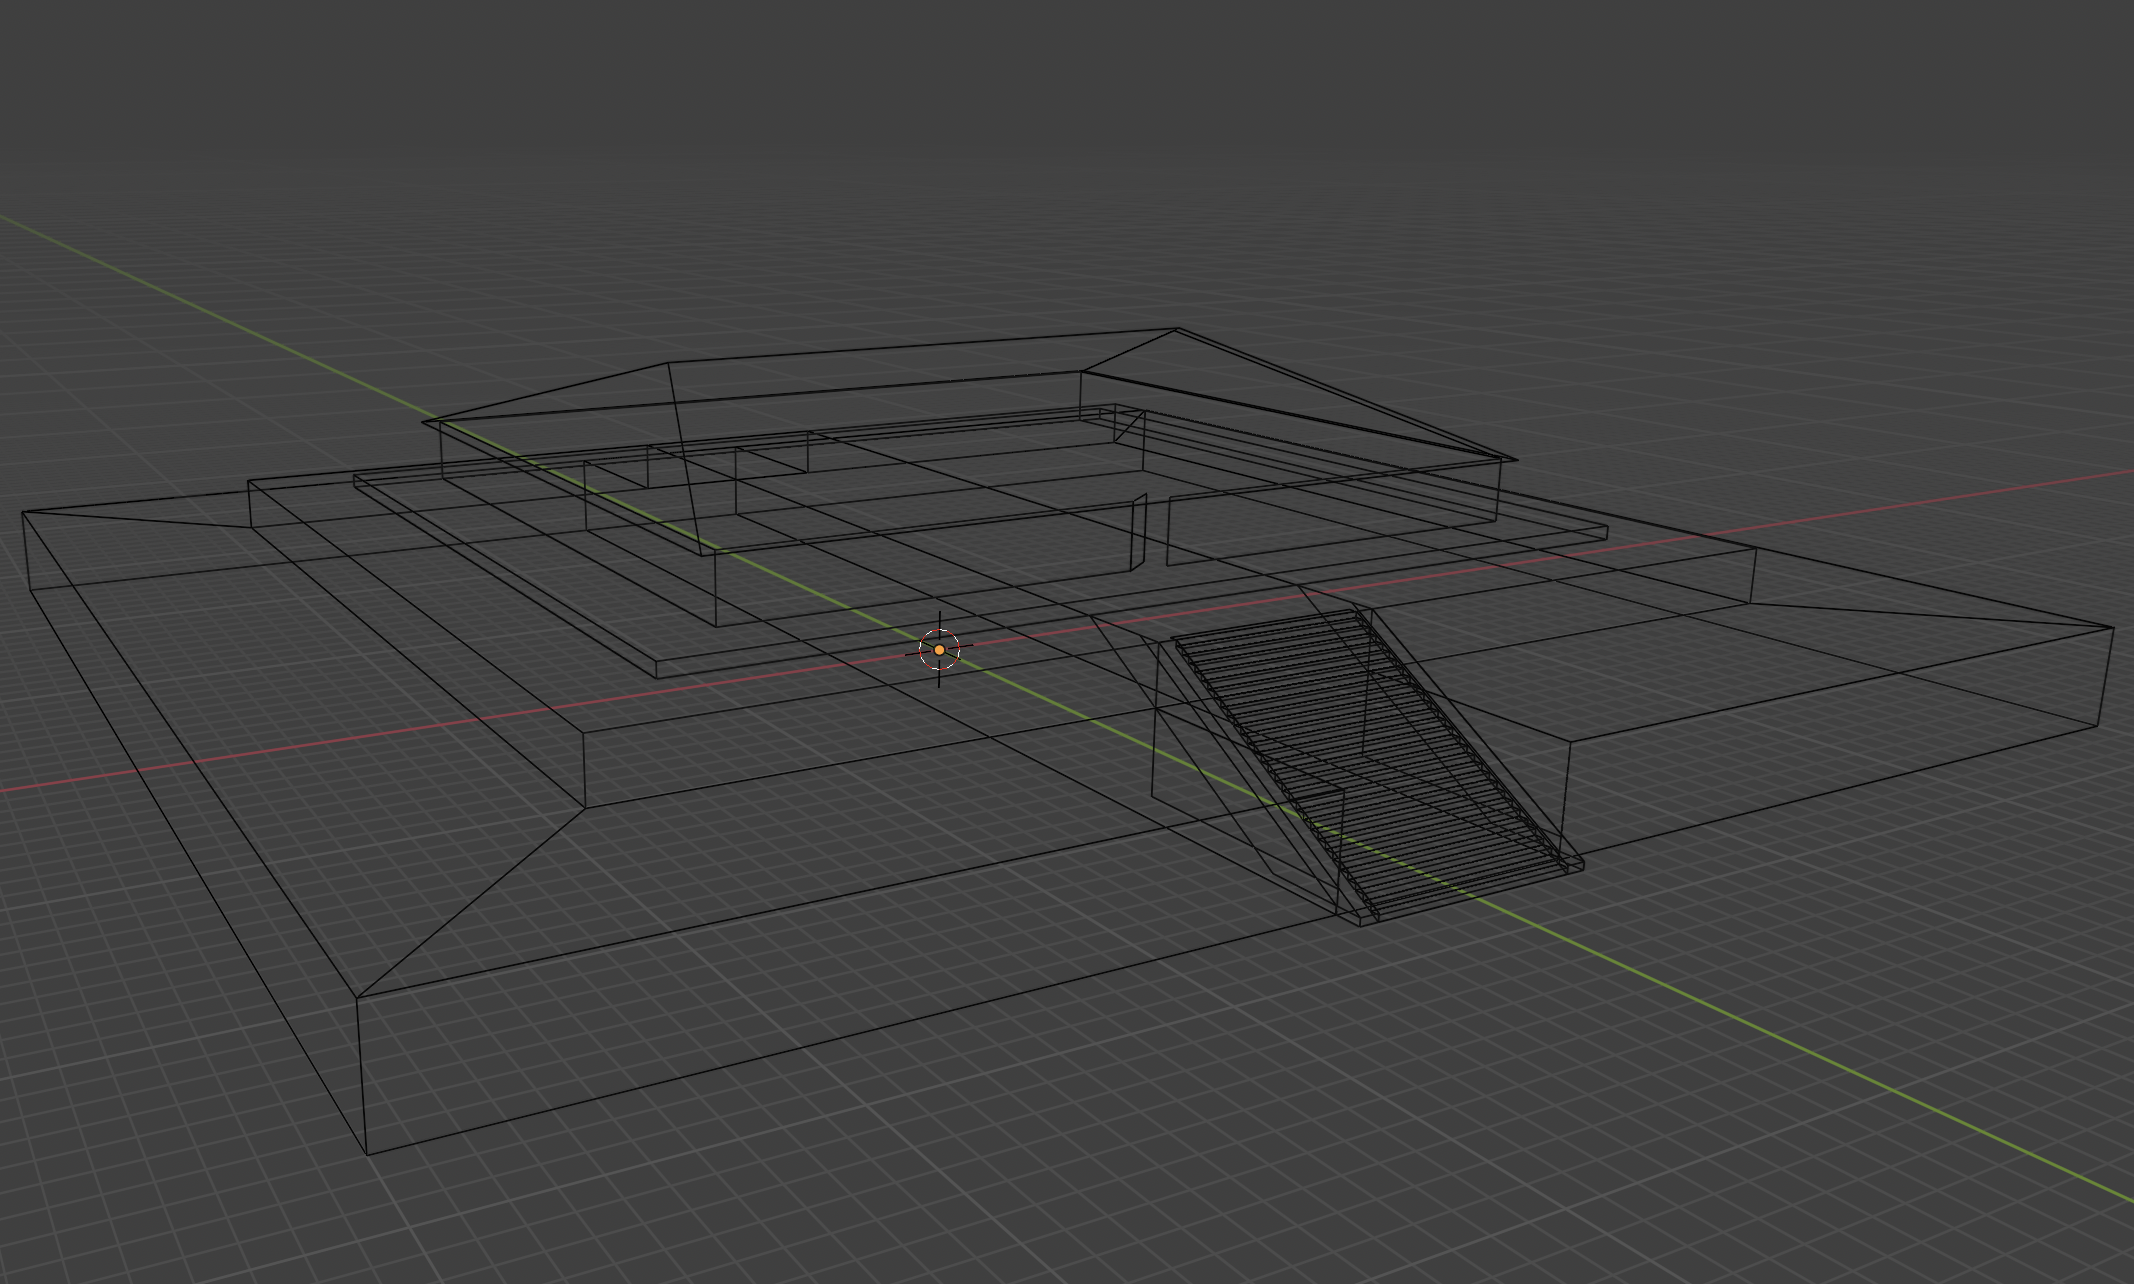
\includegraphics[width=0.85\linewidth]{resultados/figures/m12/m12_wireframe.png}
    \end{subfigure}\hfill
    \begin{subfigure}{0.48\textwidth}
        \centering
        \caption{Vista sólida sin texturas}
        \label{fig:m12-solid}
        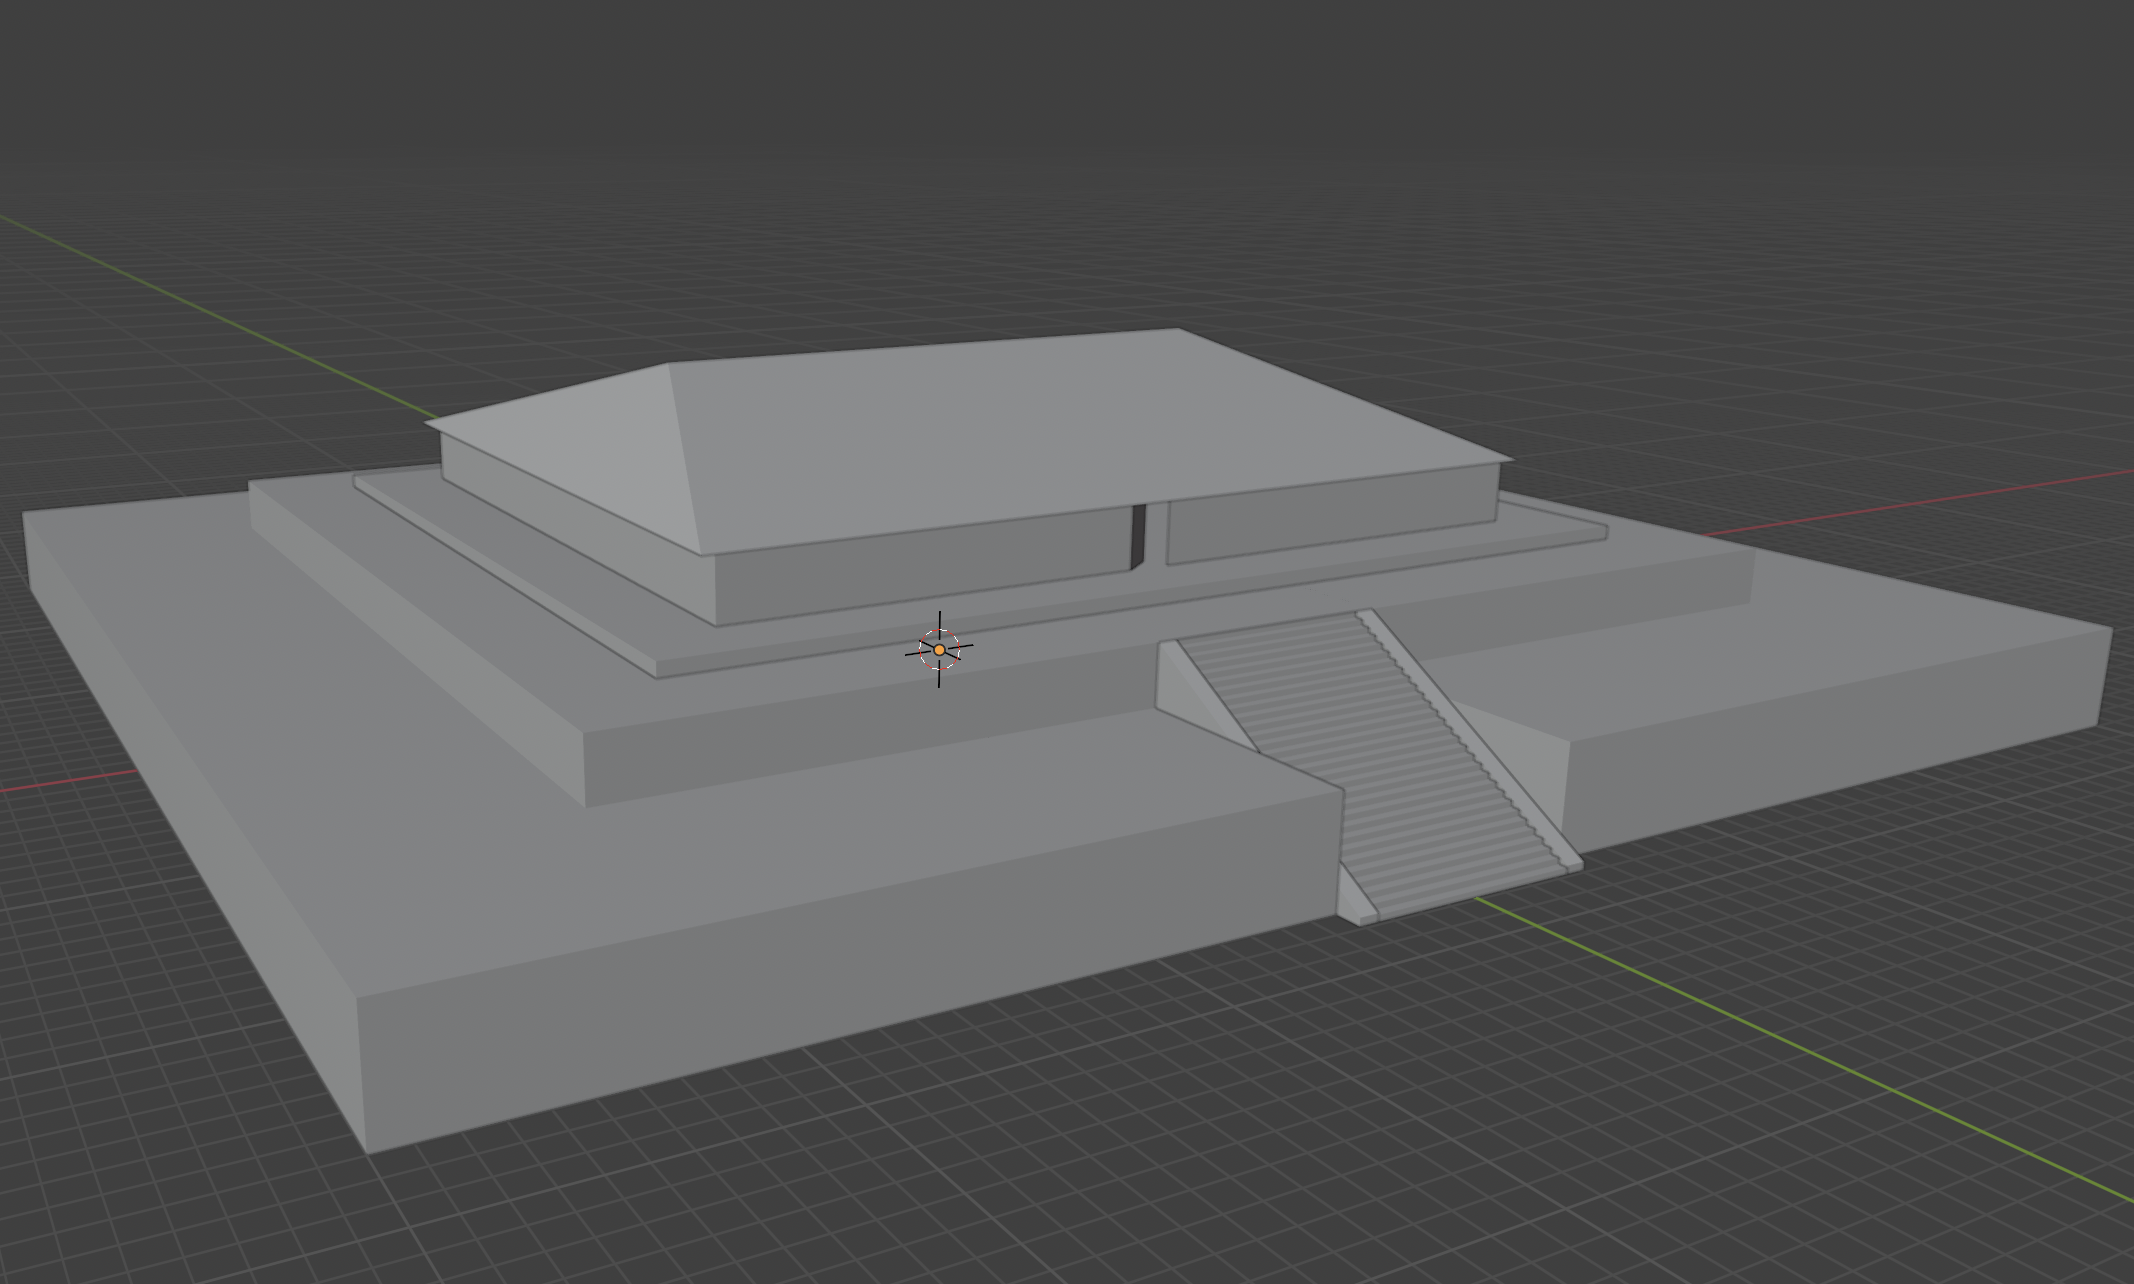
\includegraphics[width=0.85\linewidth]{resultados/figures/m12/m12_solid.png}
    \end{subfigure}

    \vspace{0.1em}

    % ----- Fila 2 -----
    \begin{subfigure}{0.48\textwidth}
        \centering
        \caption{Vista con materiales/texturas}
        \label{fig:m12-textured}
        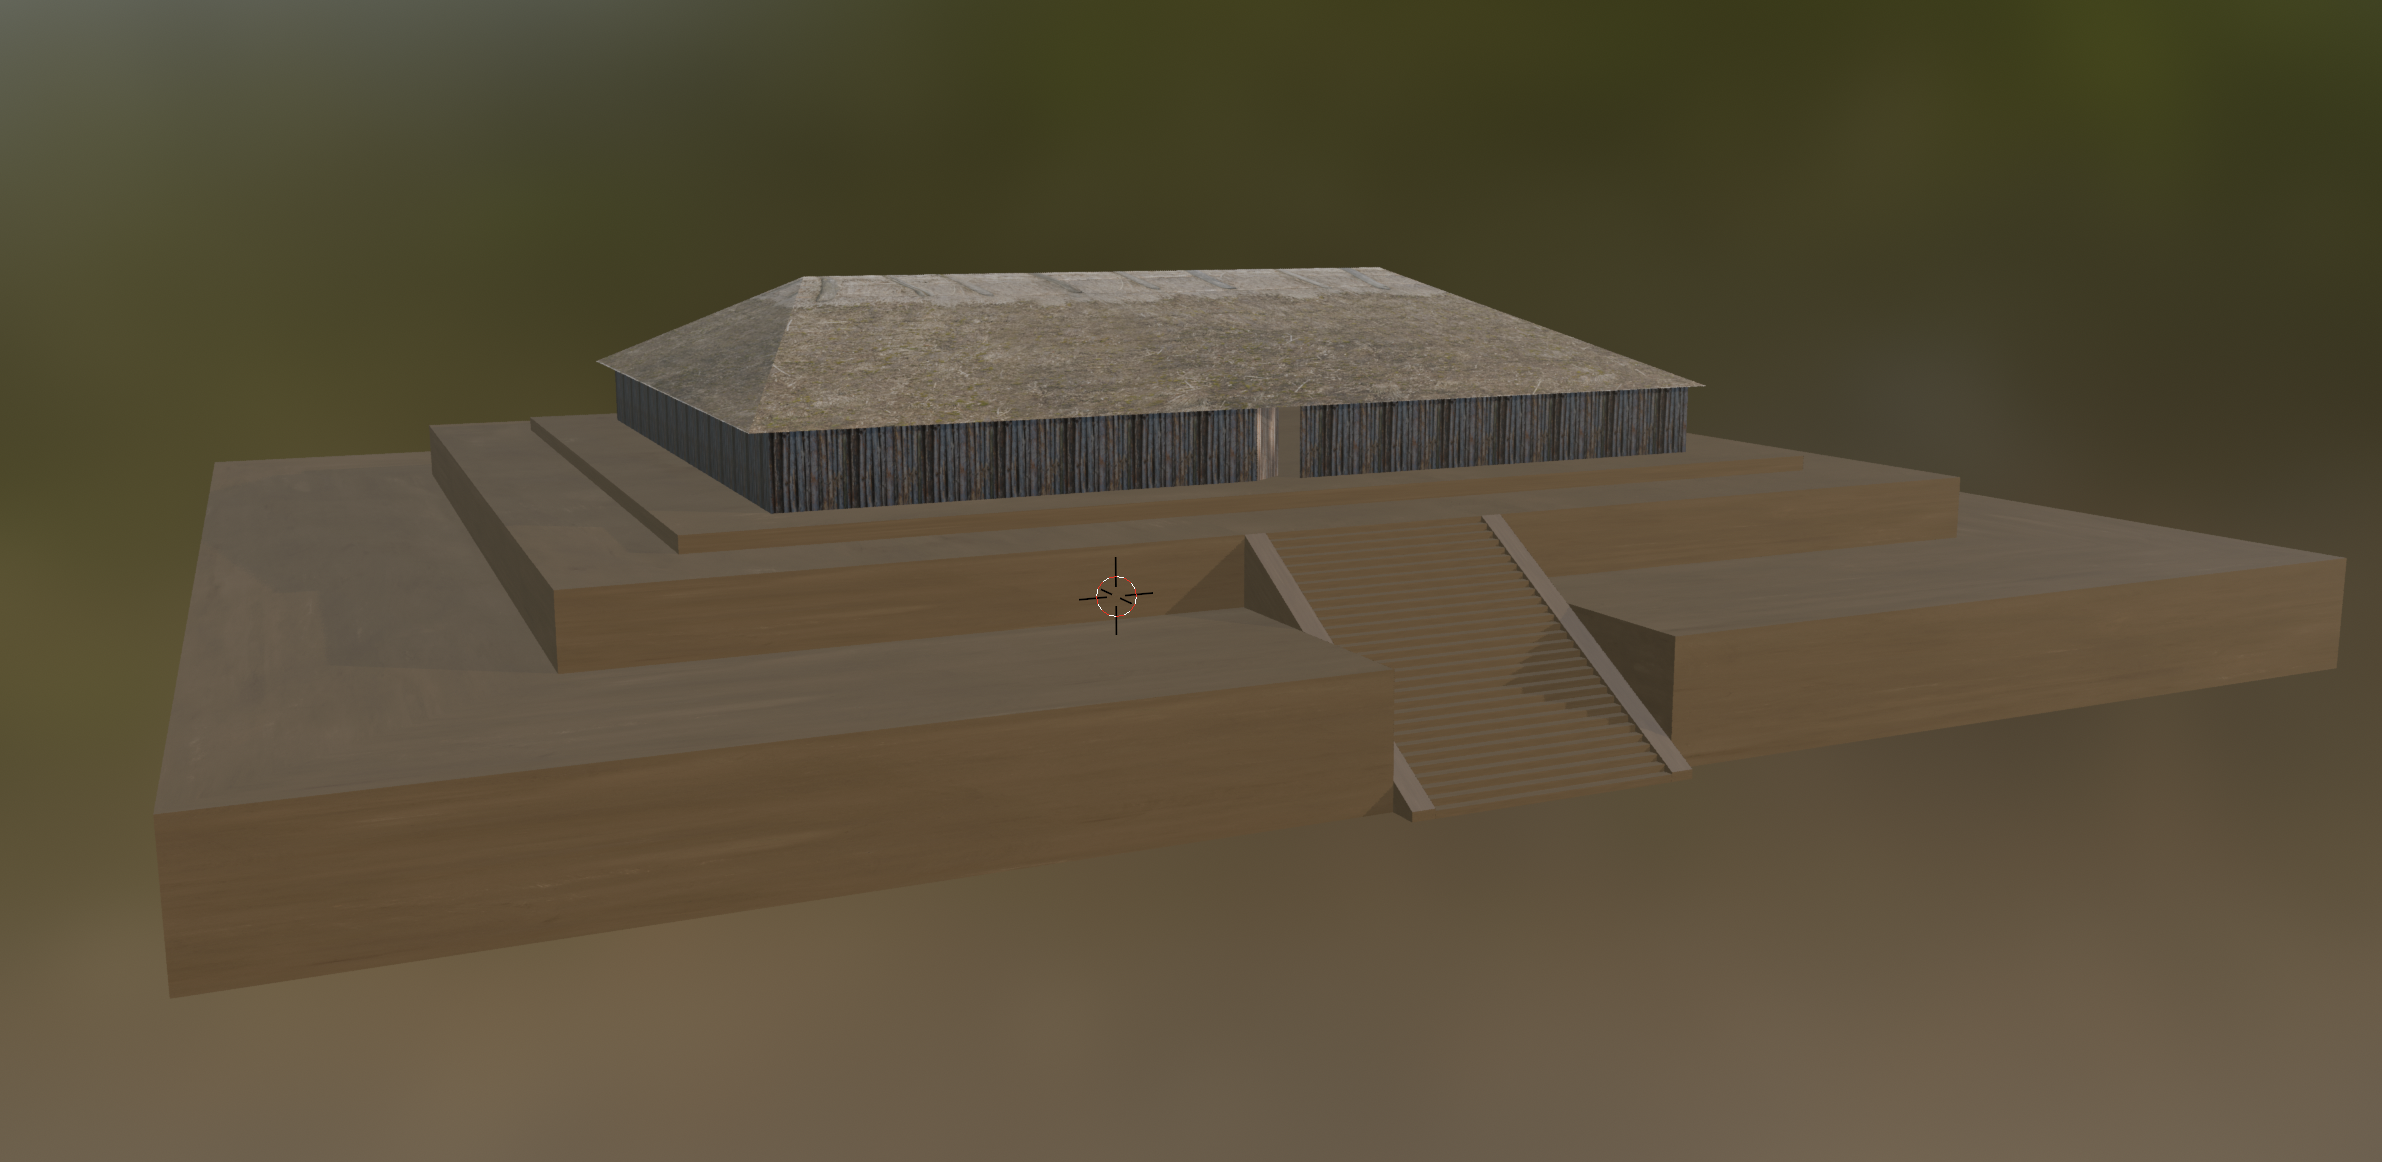
\includegraphics[width=0.85\linewidth]{resultados/figures/m12/m12_textured_viewport.png}
    \end{subfigure}
\end{figure}

\begin{figure}[!htbp]
    \centering
    \caption{Montículo 12 visualizado en la aplicación de realidad aumentada, mostrando la reconstrucción superpuesta en el entorno real del parque arqueológico}
    \label{fig:m12-ar}
    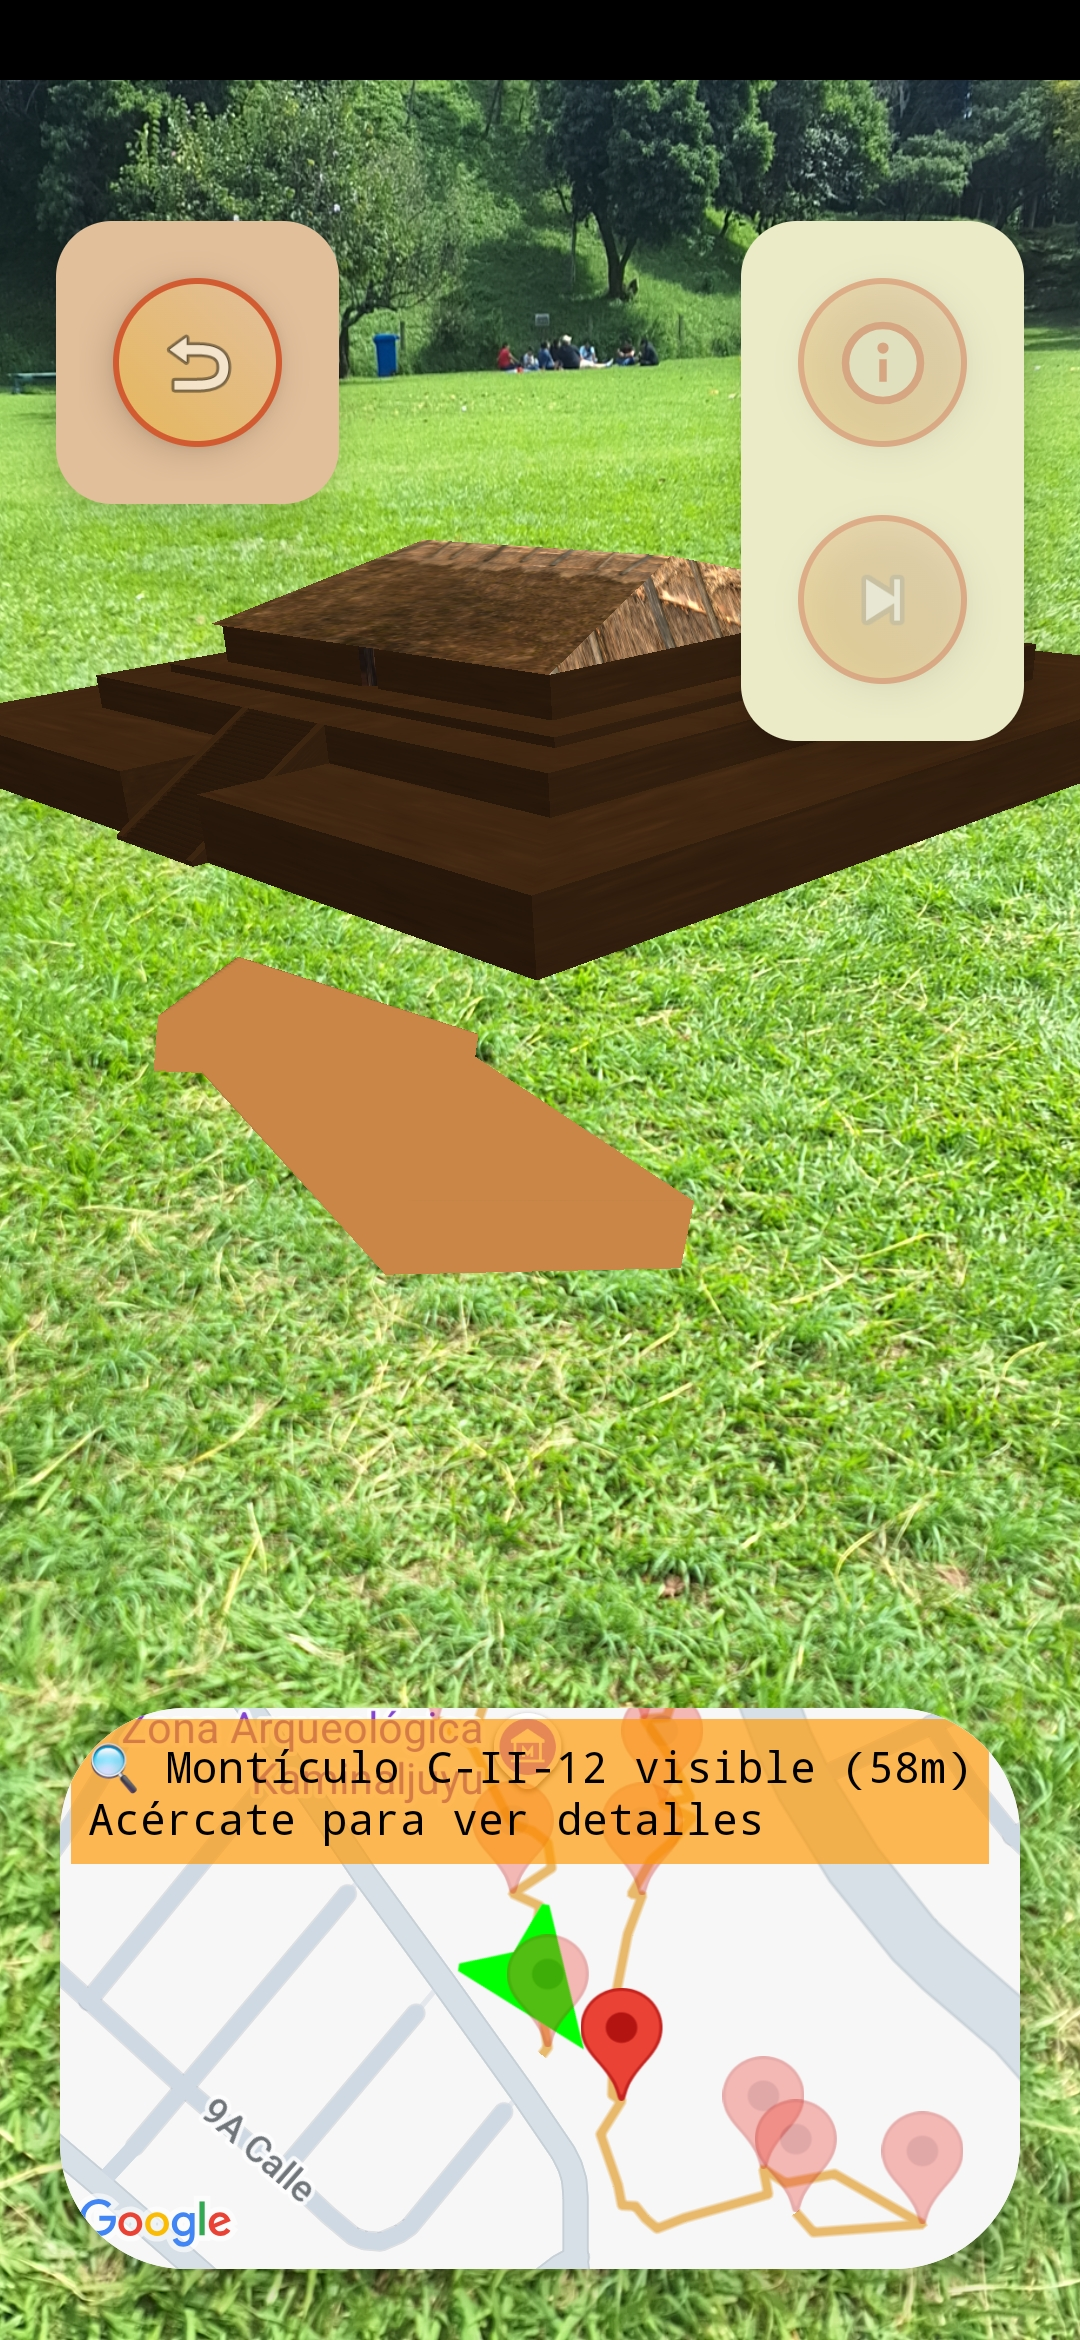
\includegraphics[width=0.28\linewidth]{resultados/figures/m12/m12_ar.jpg}
\end{figure}
\FloatBarrier
\clearpage
\FloatBarrier
\subsection{Montículo 13}

\begin{figure}[!htbp]
    \centering
    \caption{Montículo 13, panel de vistas}
    \label{fig:m13-panel}
    % ----- Fila 1 -----
    \begin{subfigure}{0.48\textwidth}
        \centering
        \caption{Vista en malla (wireframe)}
        \label{fig:m13-wire}
        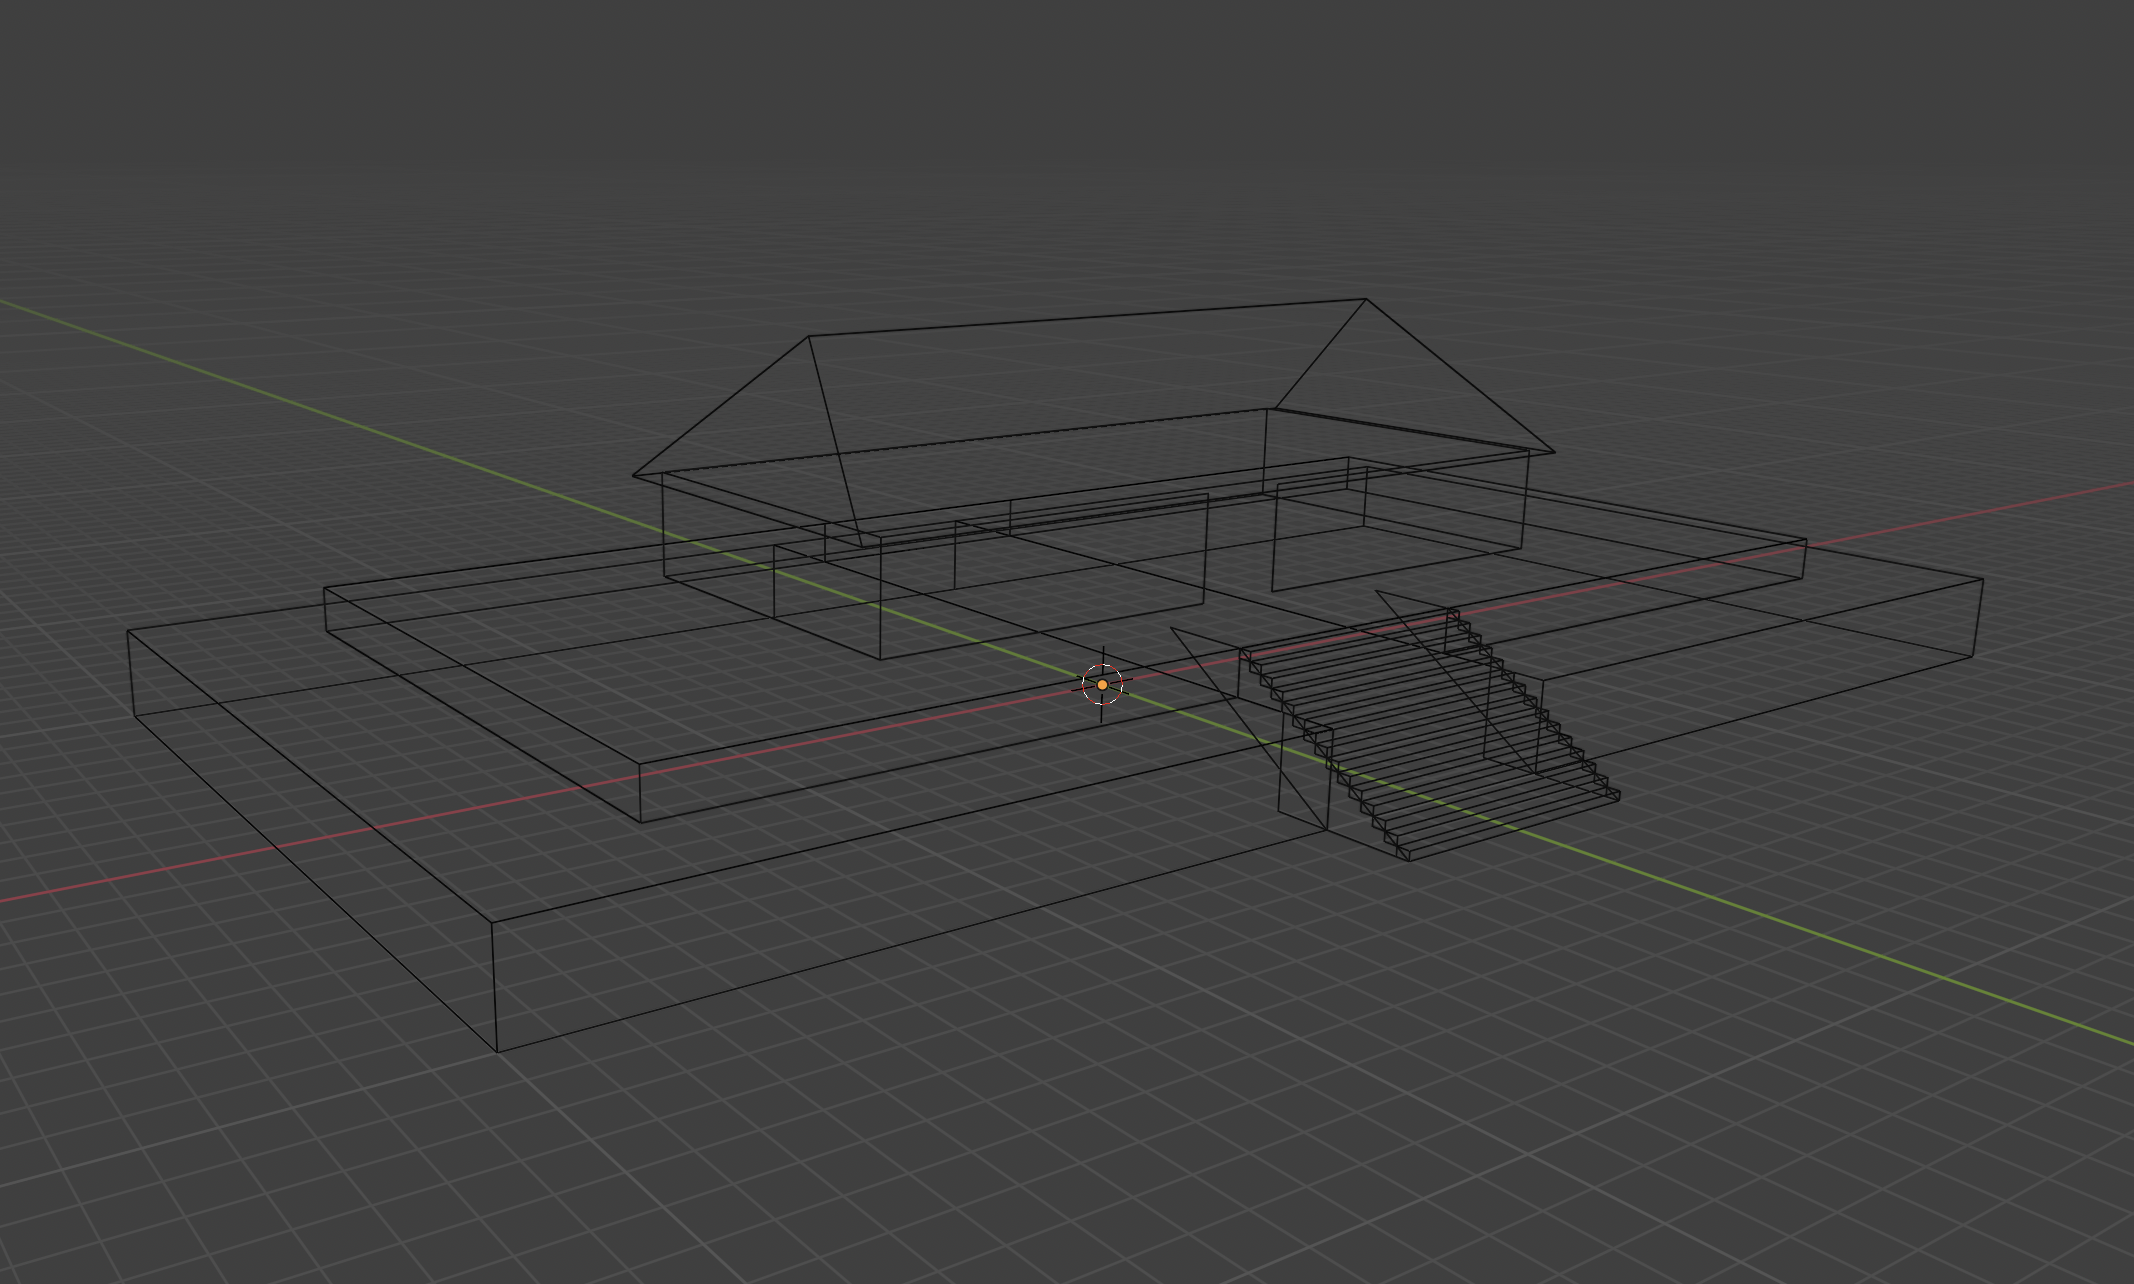
\includegraphics[width=0.85\linewidth]{resultados/figures/m13/m13_wireframe.png}
    \end{subfigure}\hfill
    \begin{subfigure}{0.48\textwidth}
        \centering
        \caption{Vista sólida sin texturas}
        \label{fig:m13-solid}
        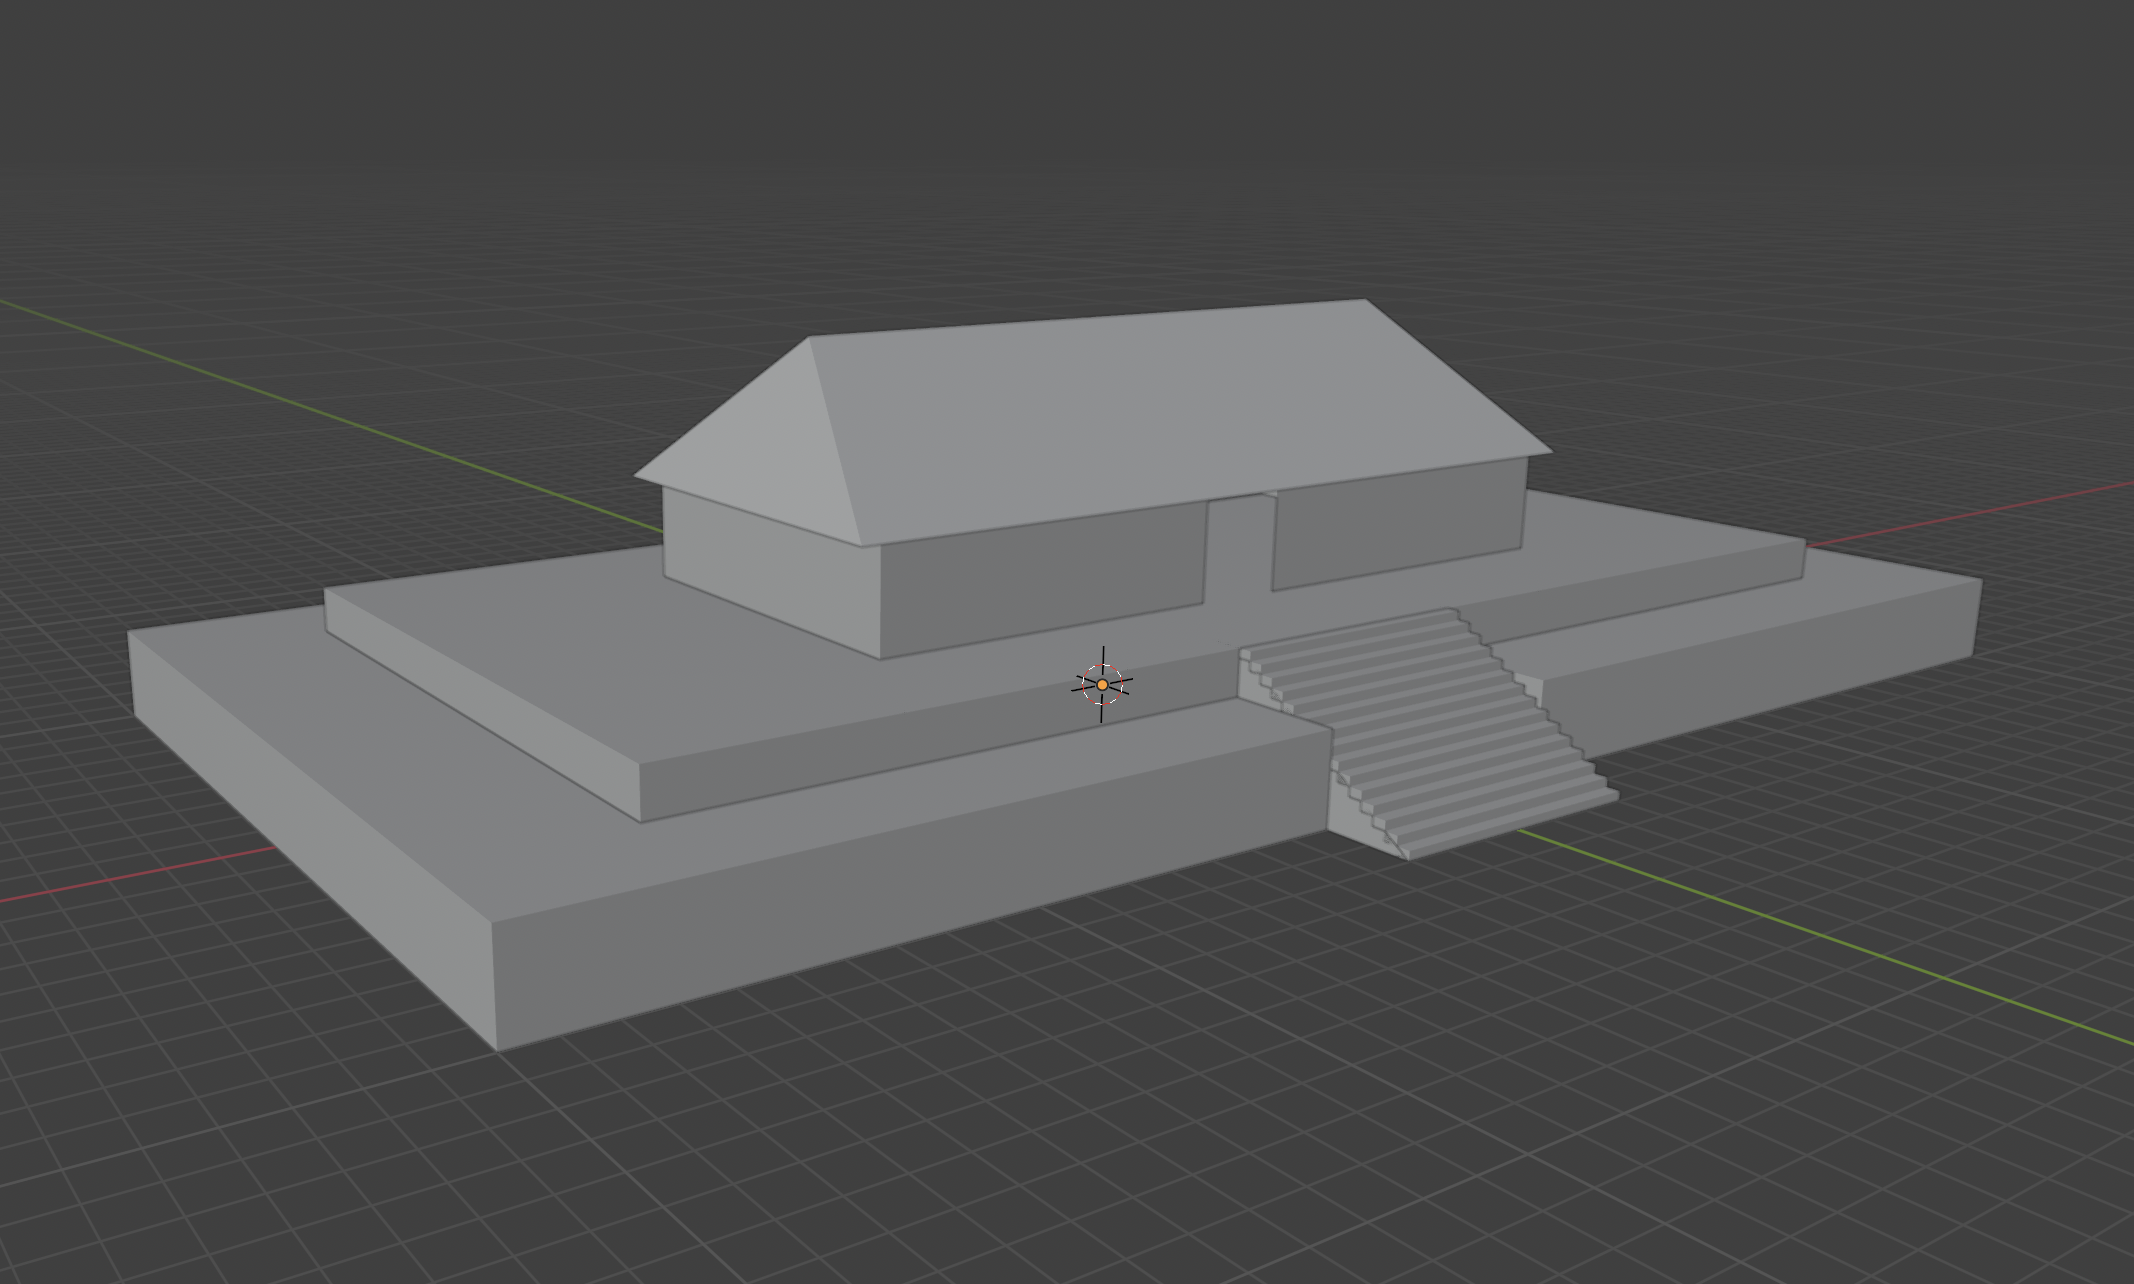
\includegraphics[width=0.85\linewidth]{resultados/figures/m13/m13_solid.png}
    \end{subfigure}

    \vspace{0.5em}

    % ----- Fila 2 -----
    \begin{subfigure}{0.48\textwidth}
        \centering
        \caption{Vista con materiales/texturas}
        \label{fig:m13-textured}
        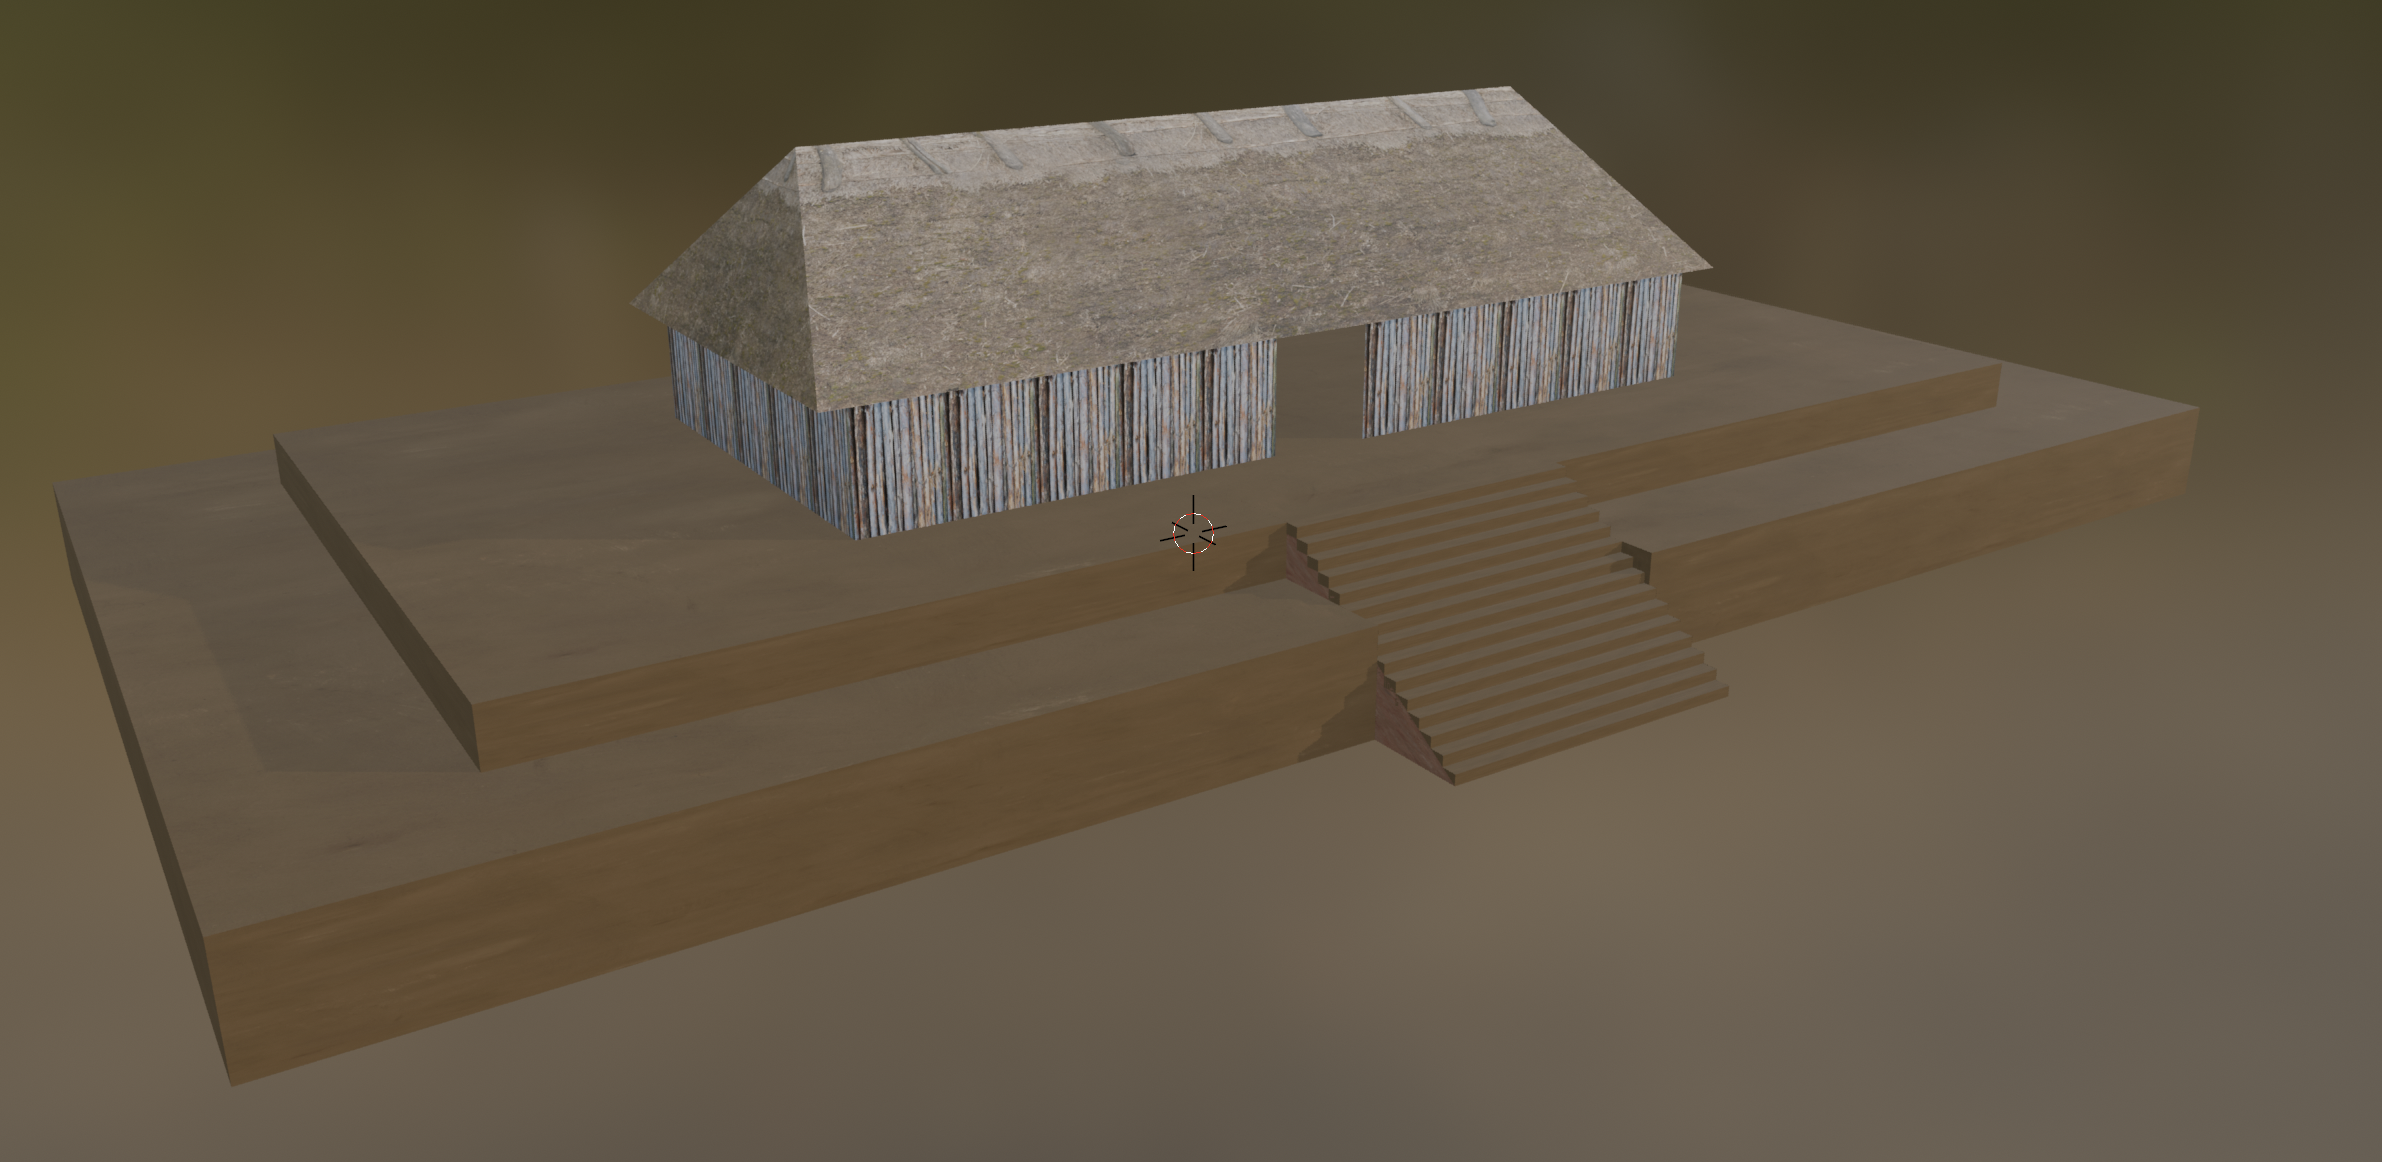
\includegraphics[width=0.85\linewidth]{resultados/figures/m13/m13_textured_viewport.png}
    \end{subfigure}
\end{figure}

\begin{figure}[!htbp]
    \centering
    \caption{Montículo 13 visualizado en la aplicación de realidad aumentada, mostrando la reconstrucción superpuesta en el entorno real del parque arqueológico}
    \label{fig:m13-ar}
    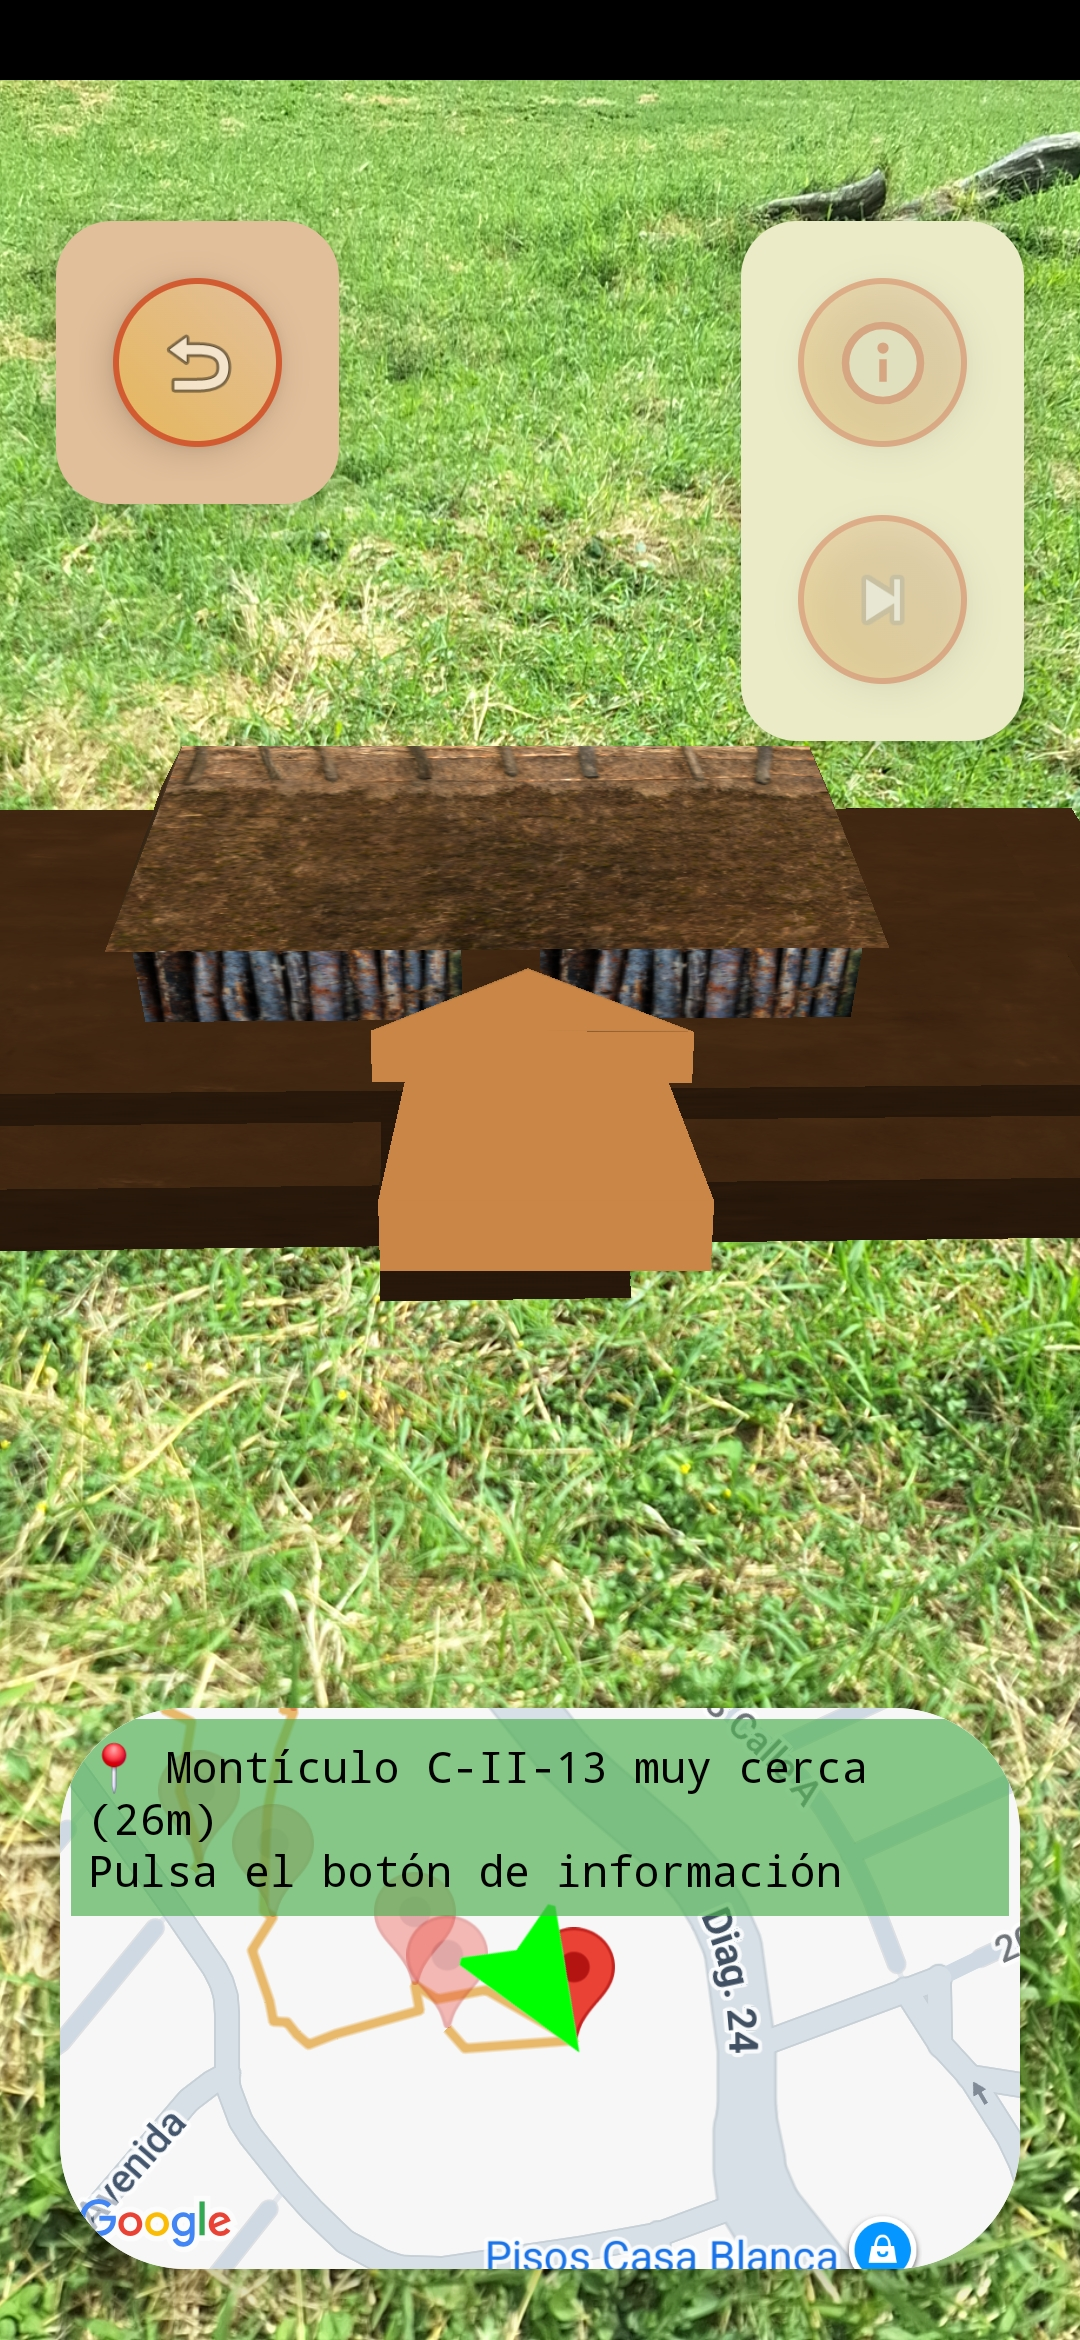
\includegraphics[width=0.28\linewidth]{resultados/figures/m13/m13_ar.jpg}
\end{figure}
\FloatBarrier
\clearpage
\FloatBarrier
\subsection{Montículo 14}

\begin{figure}[!htbp]
    \centering
    % ----- Fila 1 -----
    \begin{subfigure}{0.48\textwidth}
        \centering
        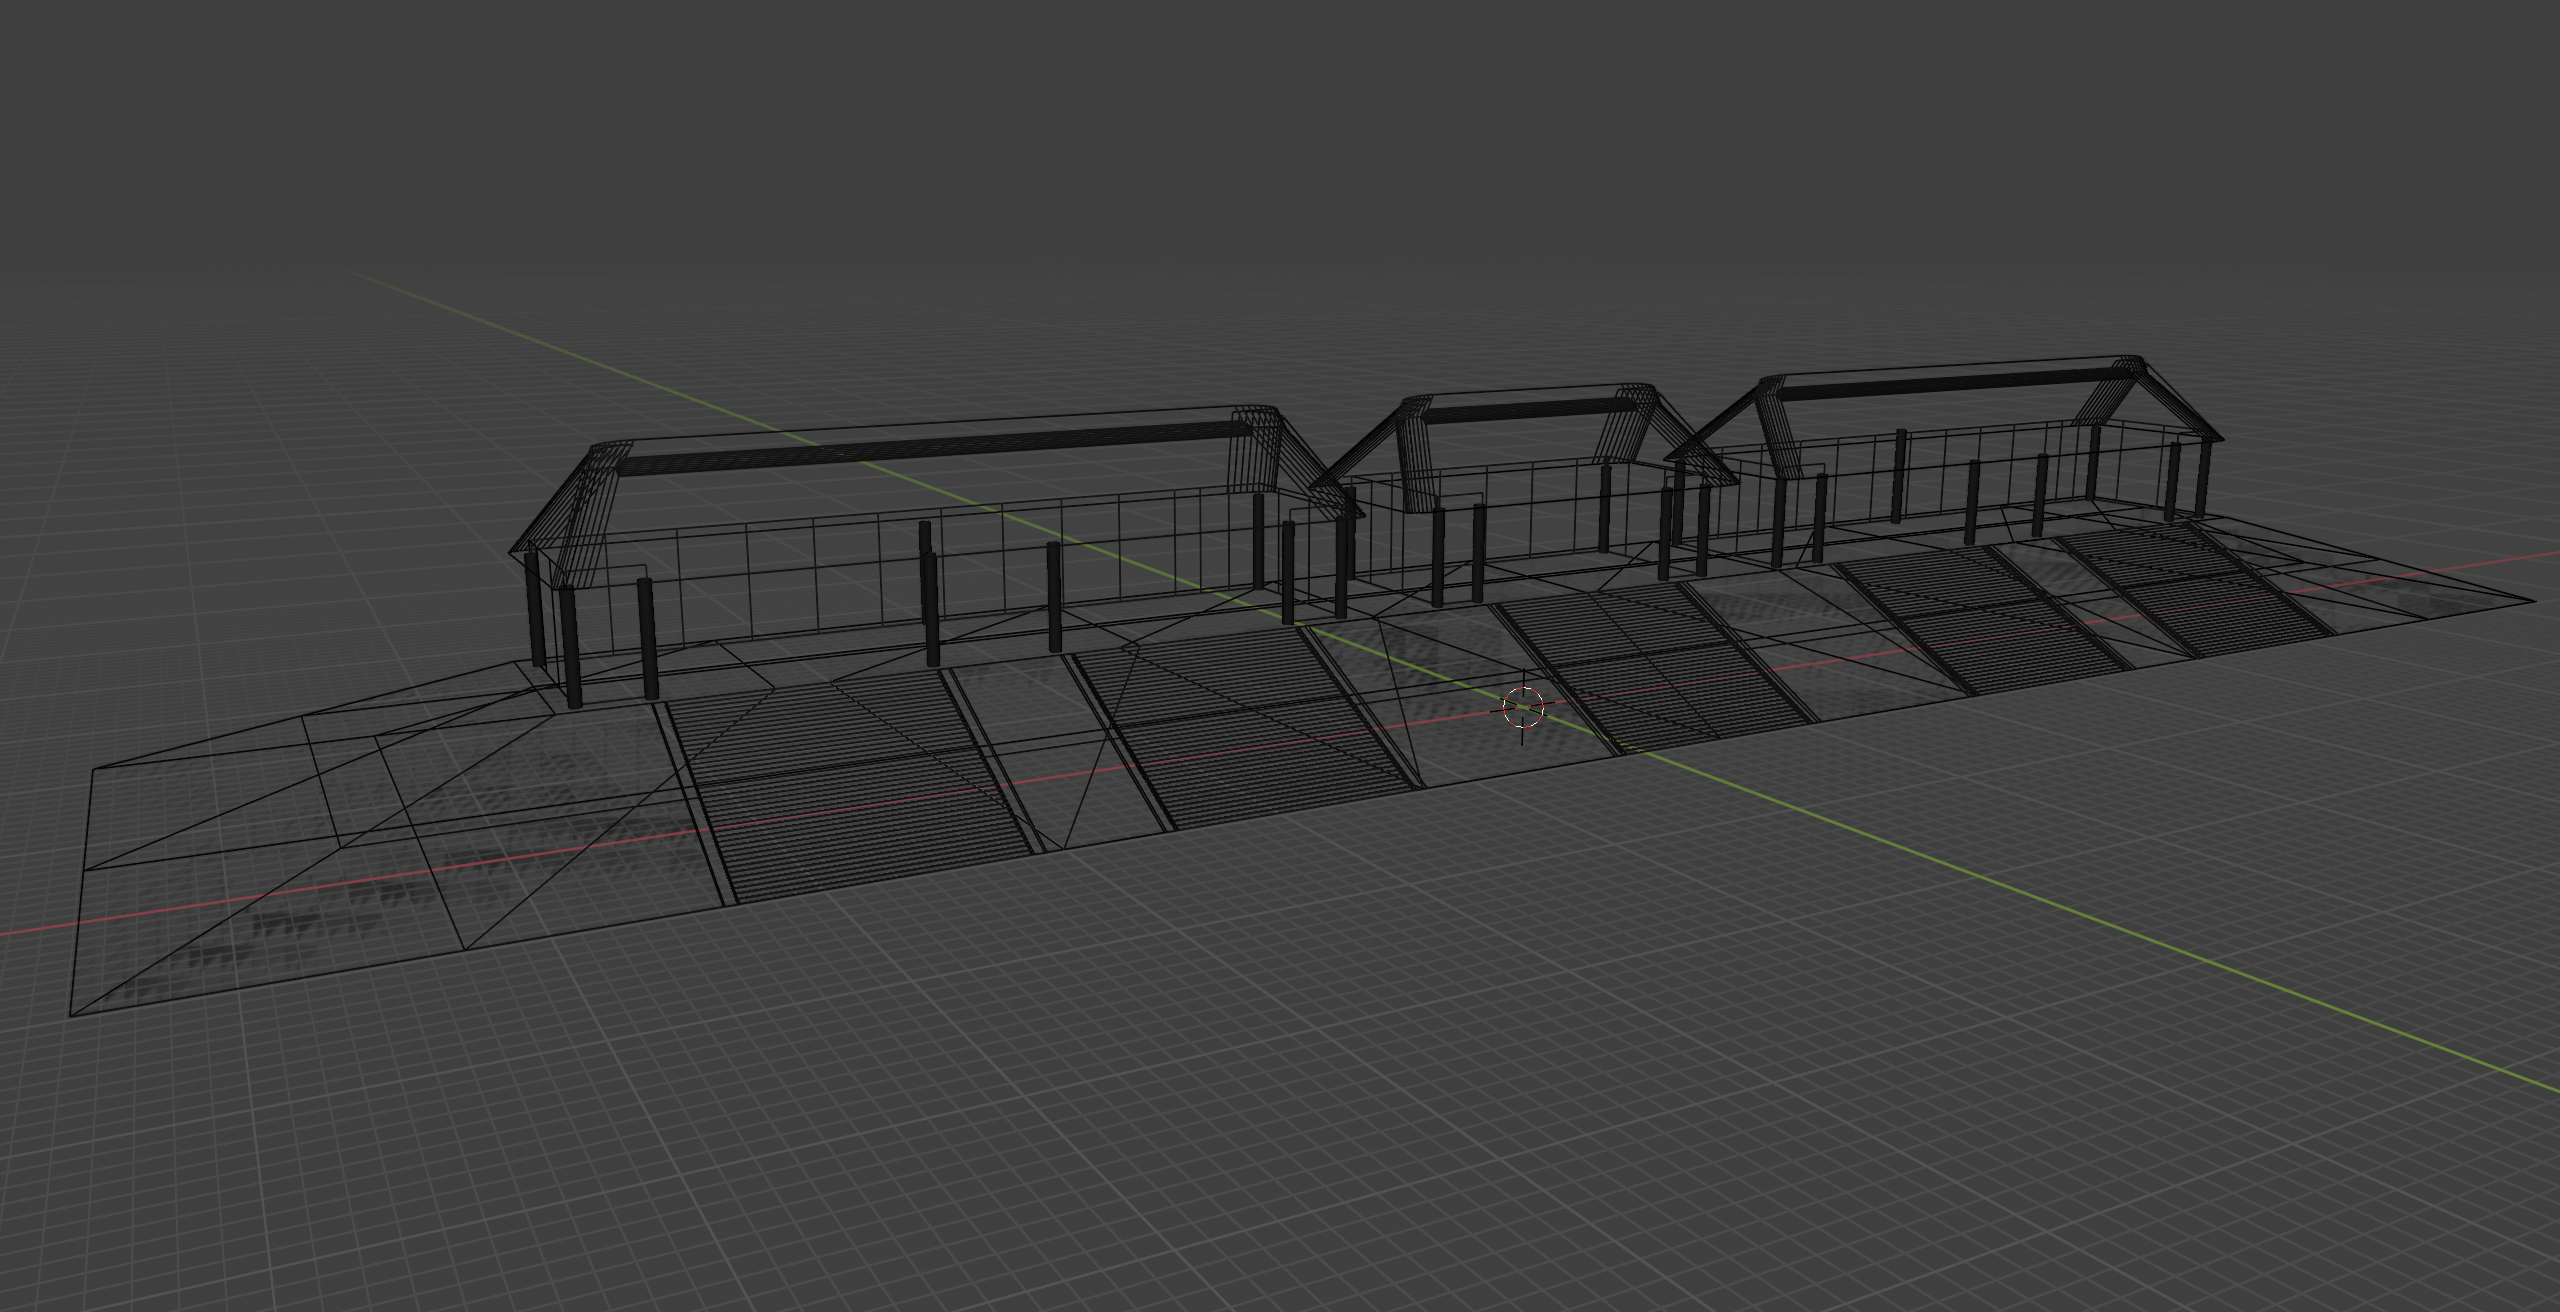
\includegraphics[width=0.85\linewidth]{resultados/figures/m14/m14_wireframe.png}
        \caption{Vista en malla (wireframe).}
        \label{fig:m14-wire}
    \end{subfigure}\hfill
    \begin{subfigure}{0.48\textwidth}
        \centering
        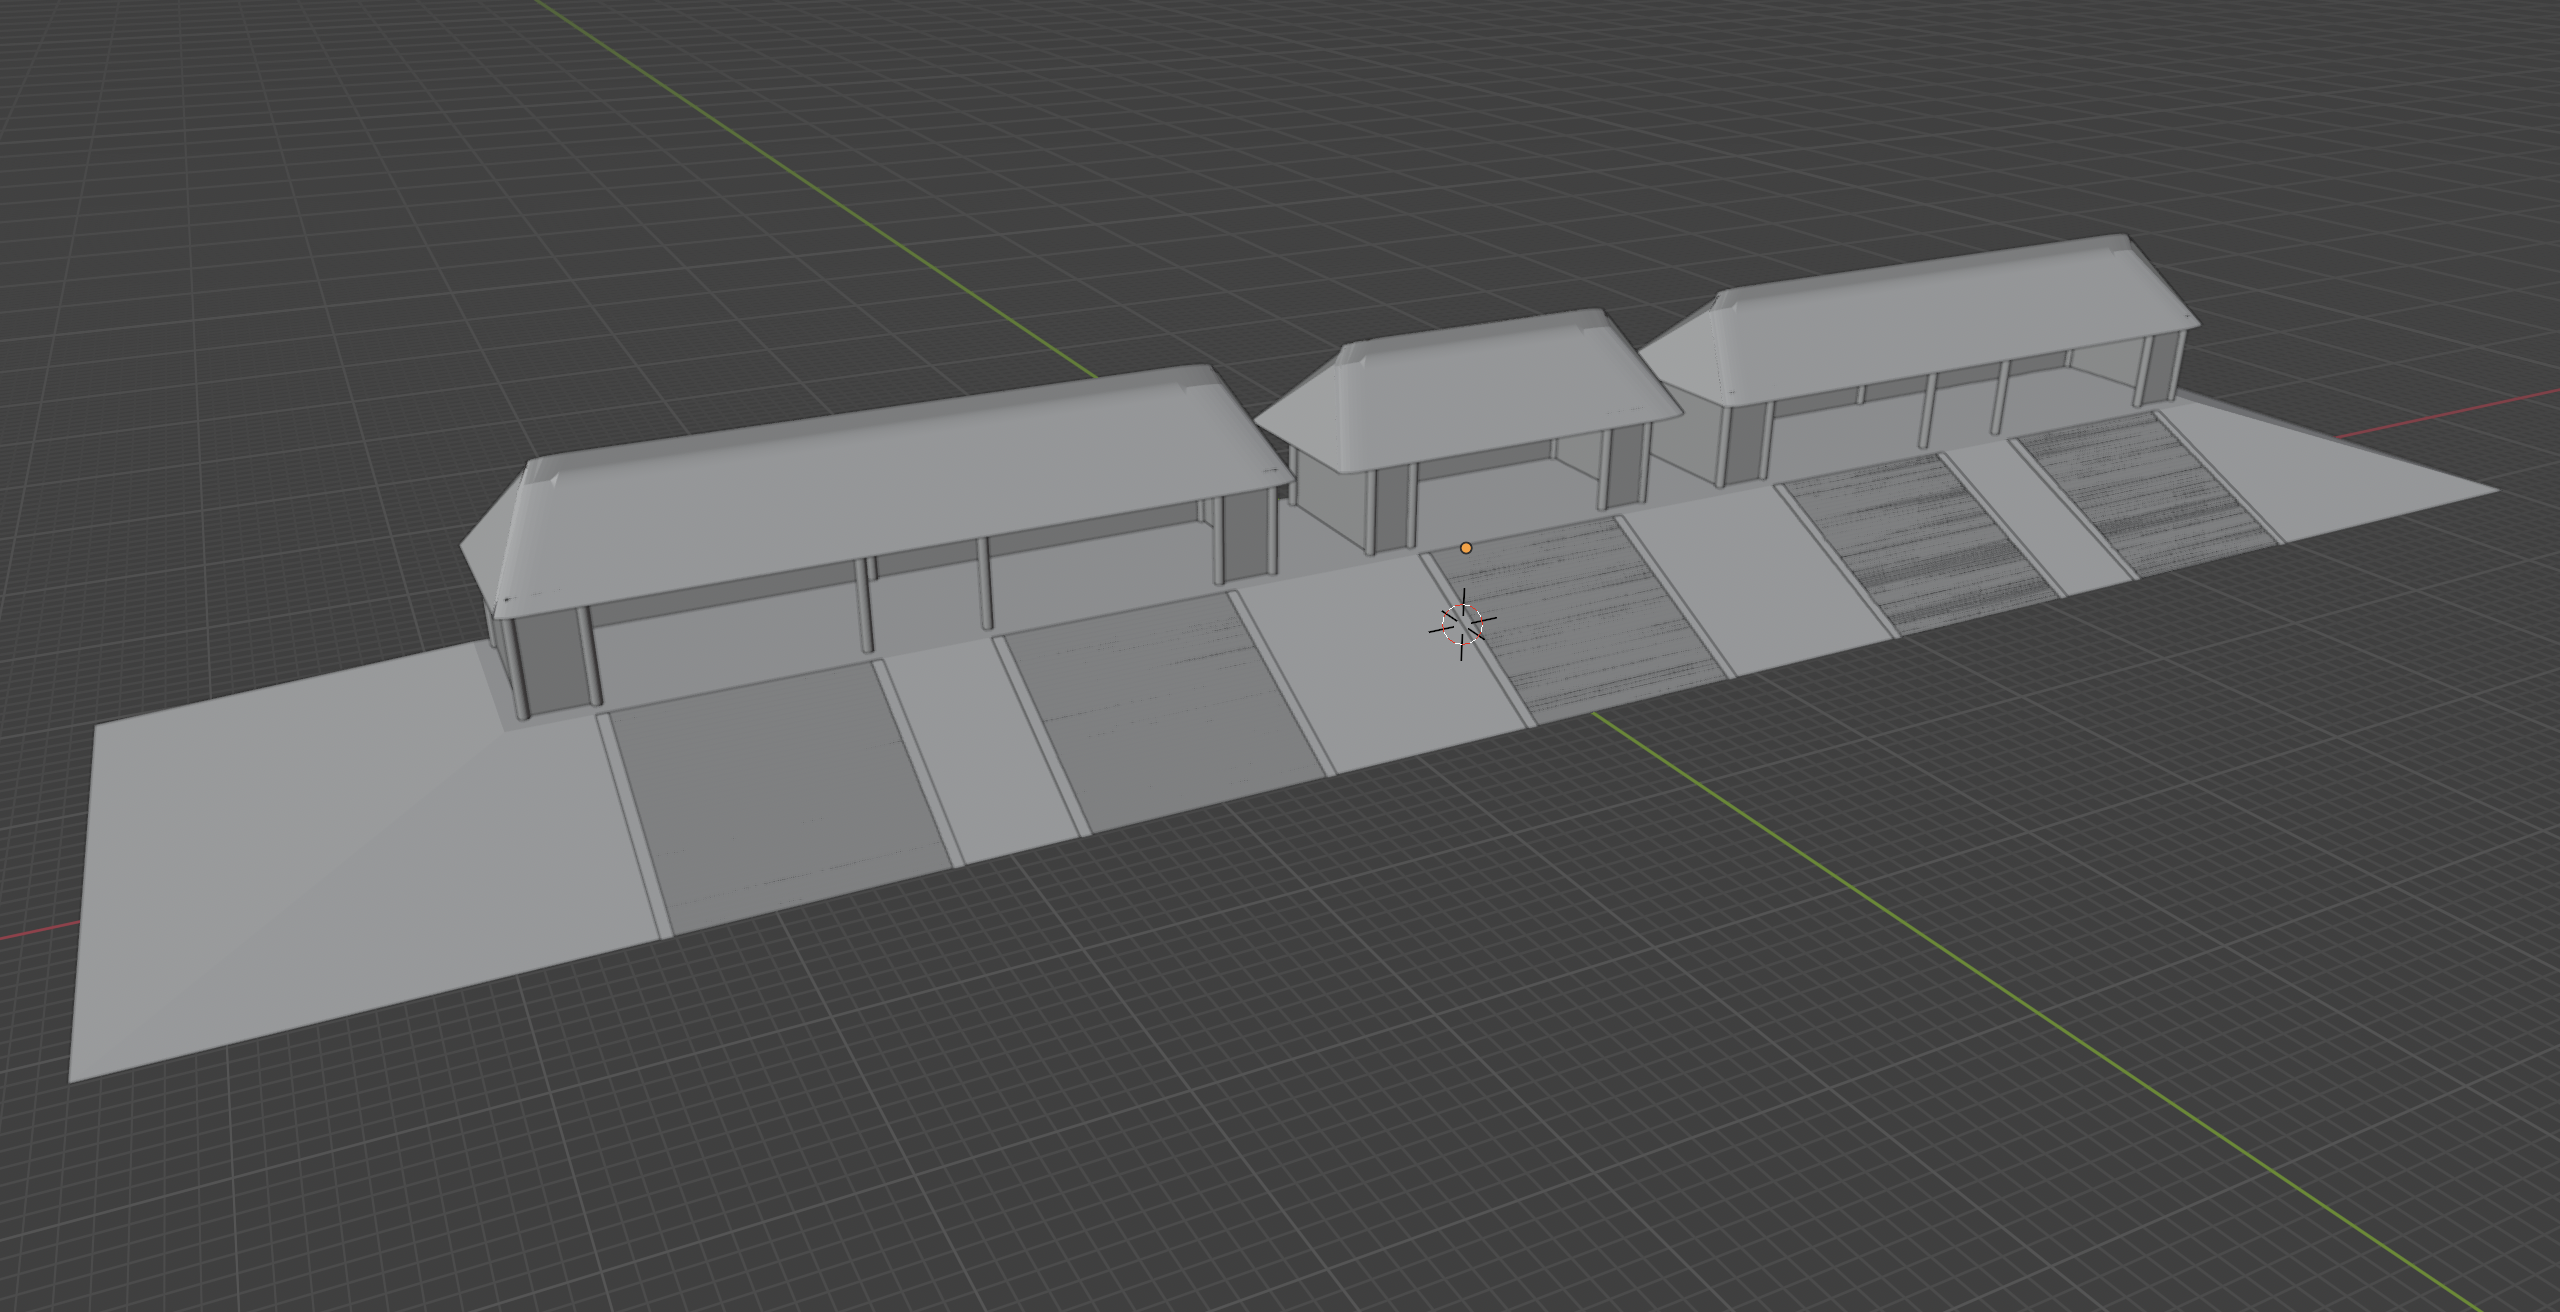
\includegraphics[width=0.85\linewidth]{resultados/figures/m14/m14_solid.png}
        \caption{Vista sólida sin texturas.}
        \label{fig:m14-solid}
    \end{subfigure}

    \vspace{0.5em}

    % ----- Fila 2 -----
    \begin{subfigure}{0.48\textwidth}
        \centering
        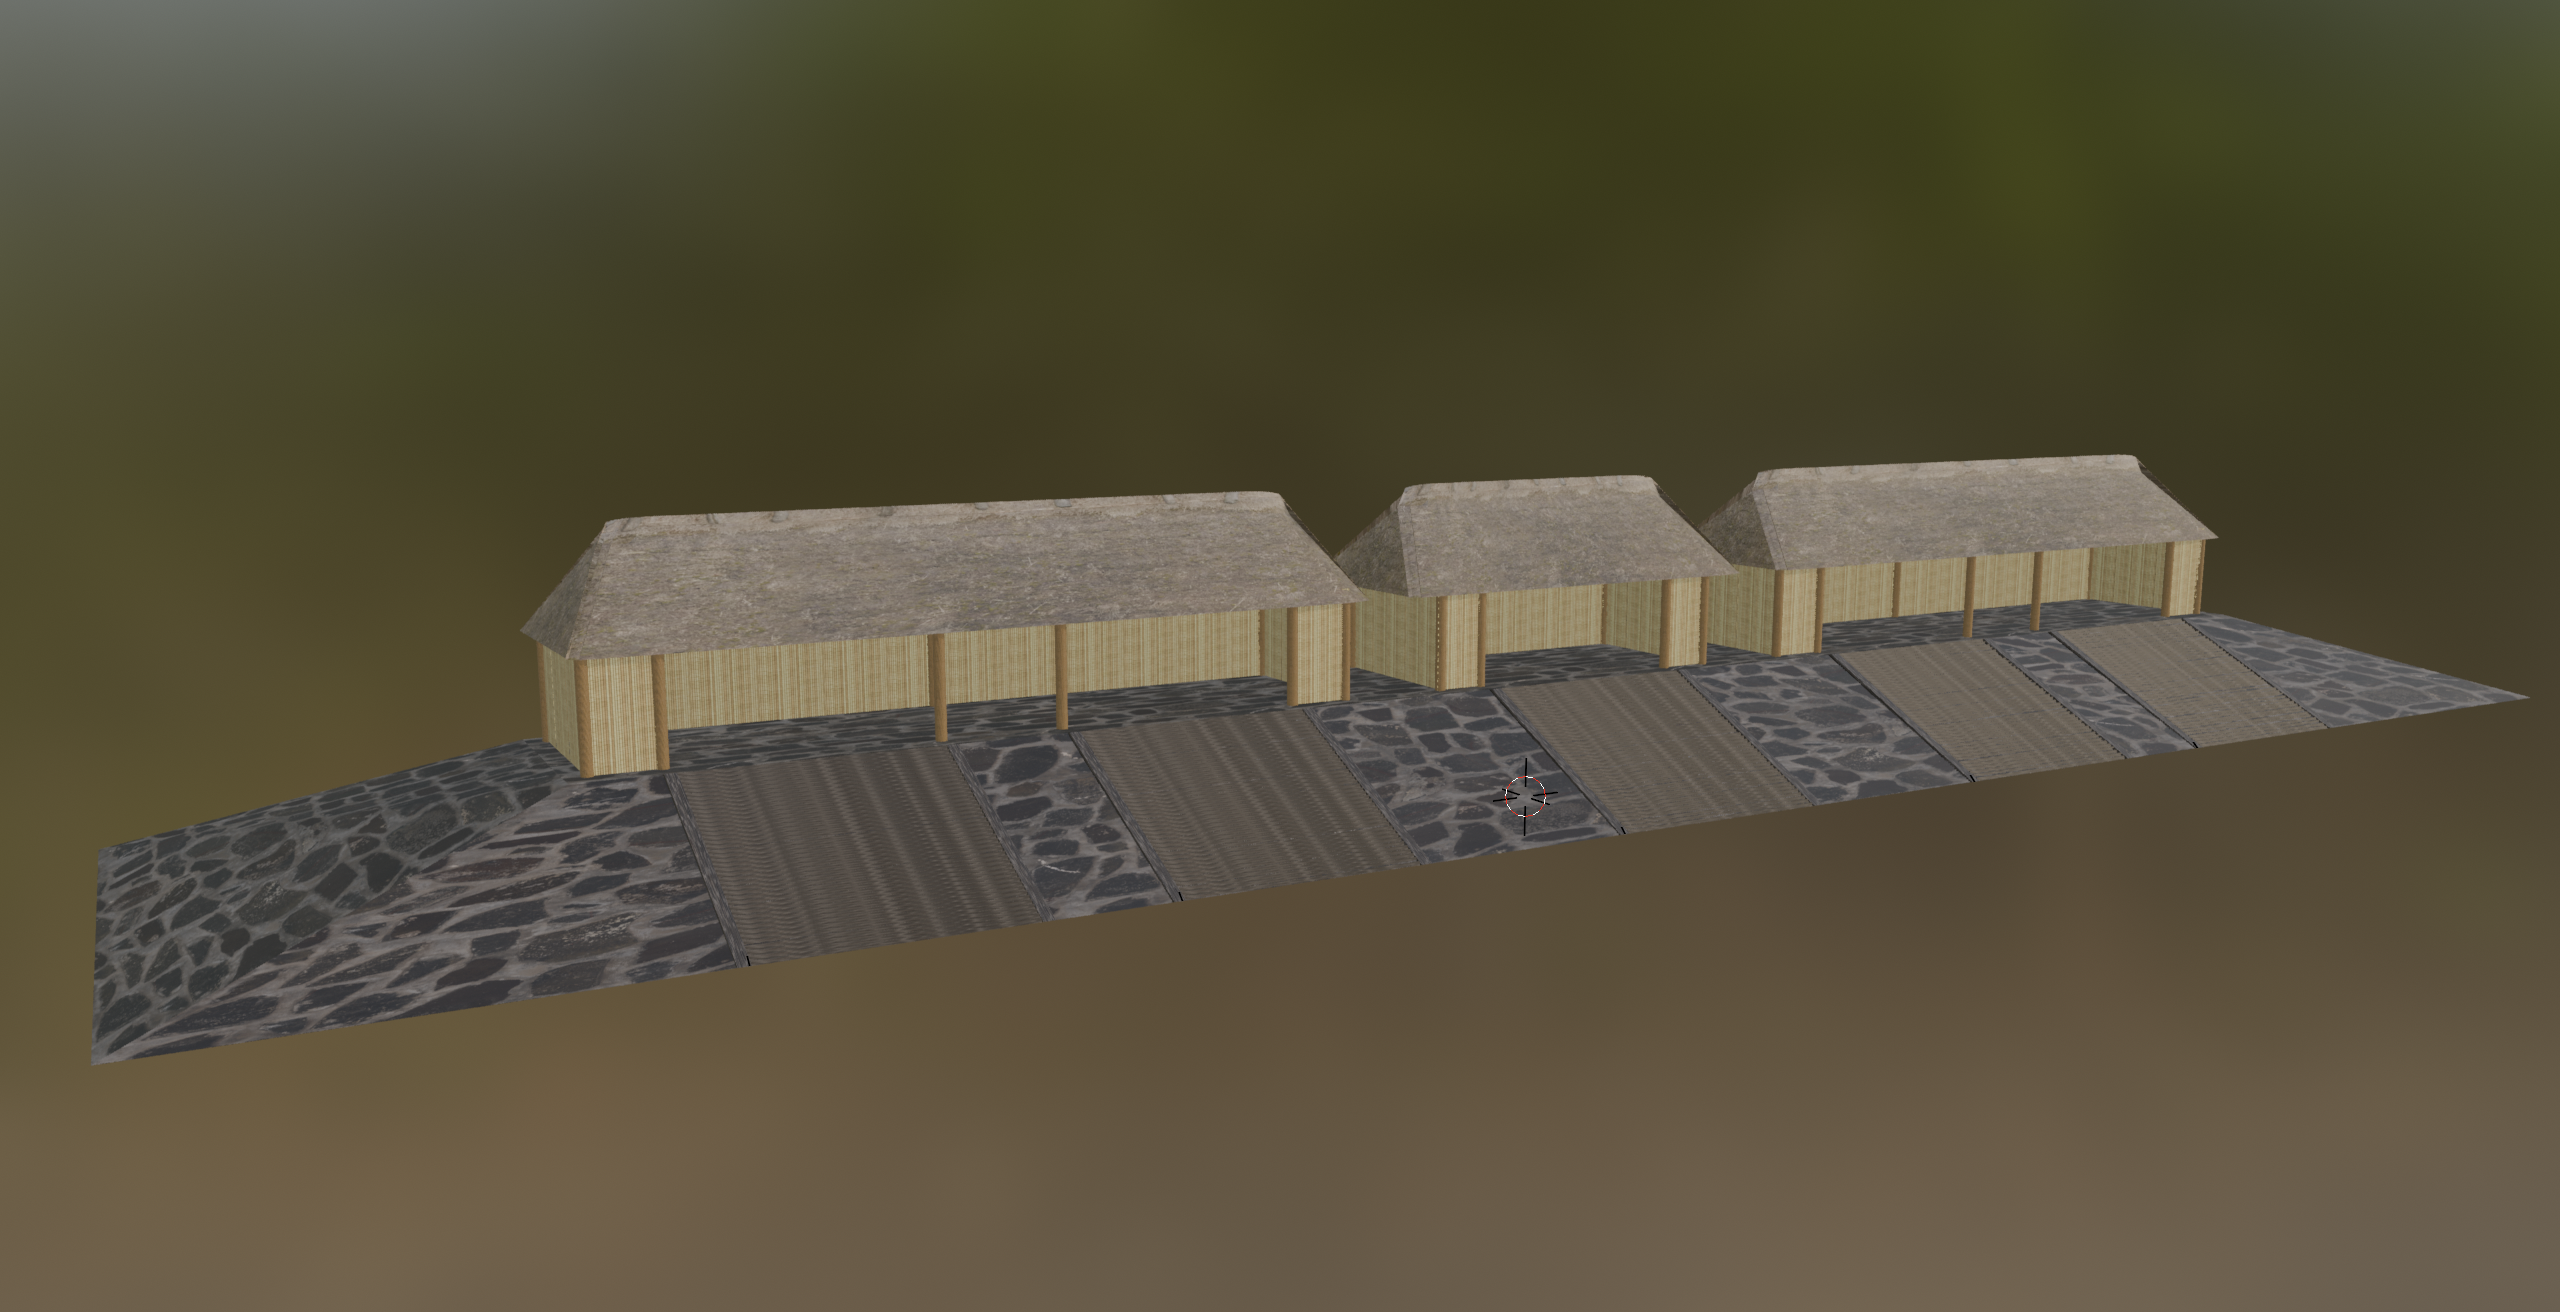
\includegraphics[width=0.85\linewidth]{resultados/figures/m14/m14_textured_viewport.png}
        \caption{Vista con materiales/texturas.}
        \label{fig:m14-textured}
    \end{subfigure}

    \caption{Montículo 14, panel de vistas.}
    \label{fig:m14-panel}
\end{figure}

\begin{figure}[!htbp]
    \centering
    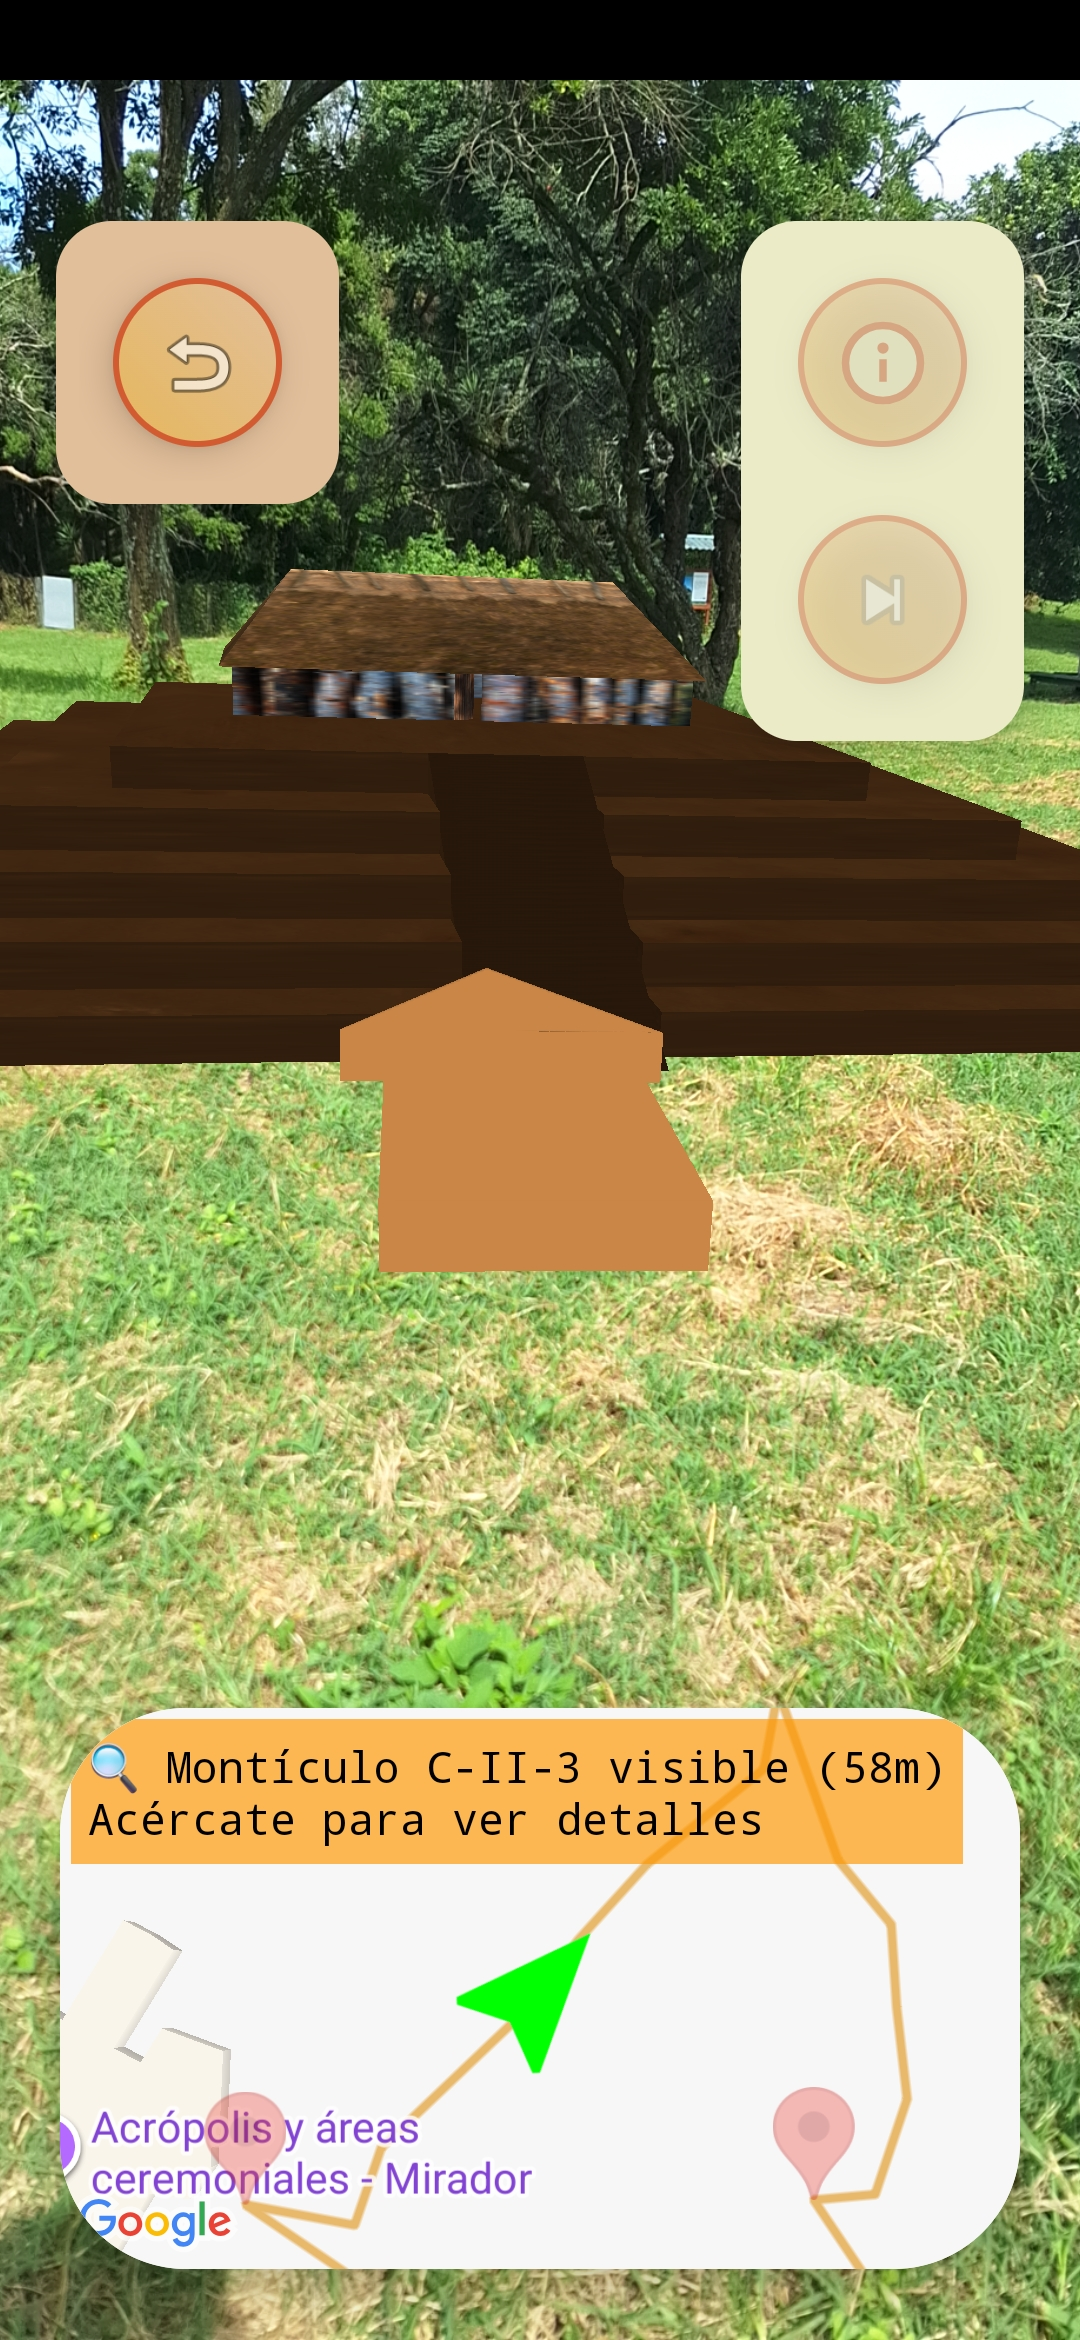
\includegraphics[width=0.28\linewidth]{resultados/figures/m3/m3_ar.jpg}
    \caption{Montículo 3 visualizado en la aplicación de realidad aumentada, mostrando la reconstrucción superpuesta en el entorno real del parque arqueológico.}
    \label{fig:m14-ar}
\end{figure}
\FloatBarrier
\clearpage
\subsection{Montículo La Palangana}
\FloatBarrier

\begin{figure}[H]
    \centering
    \caption{Montículo La Palangana, panel de vistas}
    \label{fig:palangana-panel}
    % ----- Fila 1 -----
    \begin{subfigure}{0.48\textwidth}
        \centering
        \caption{Vista en malla (wireframe)}
        \label{fig:palangana-wire}
        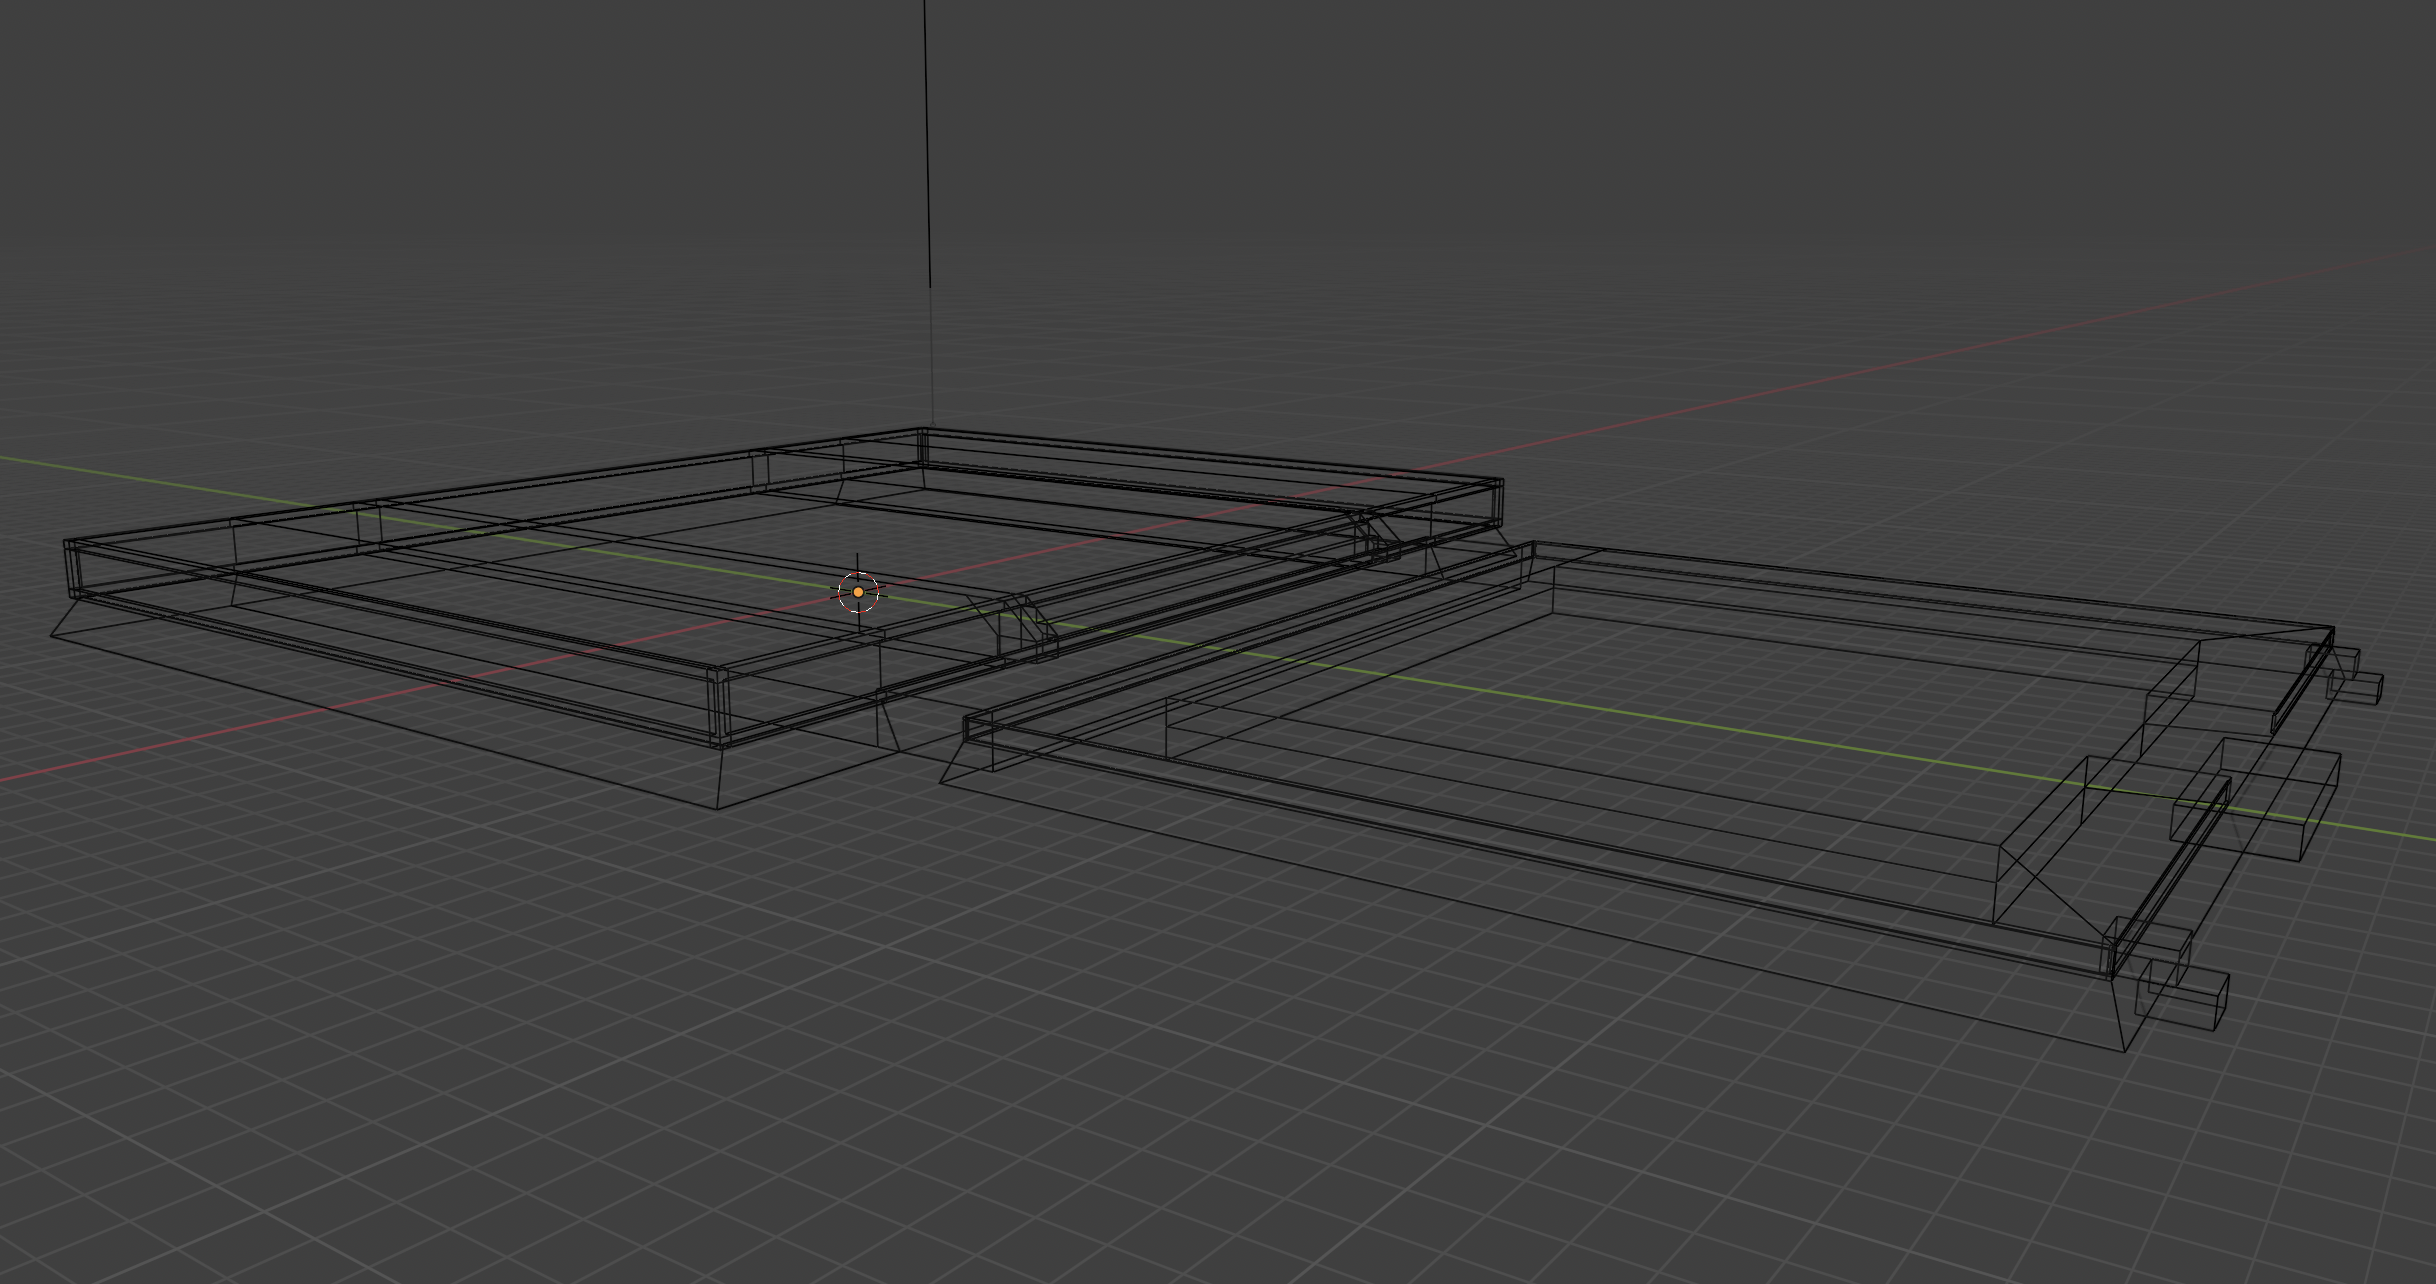
\includegraphics[width=0.85\linewidth]{resultados/figures/palangana/palangana_wireframe.png}
    \end{subfigure}\hfill
    \begin{subfigure}{0.48\textwidth}
        \centering
        \caption{Vista sólida sin texturas}
        \label{fig:palangana-solid}
        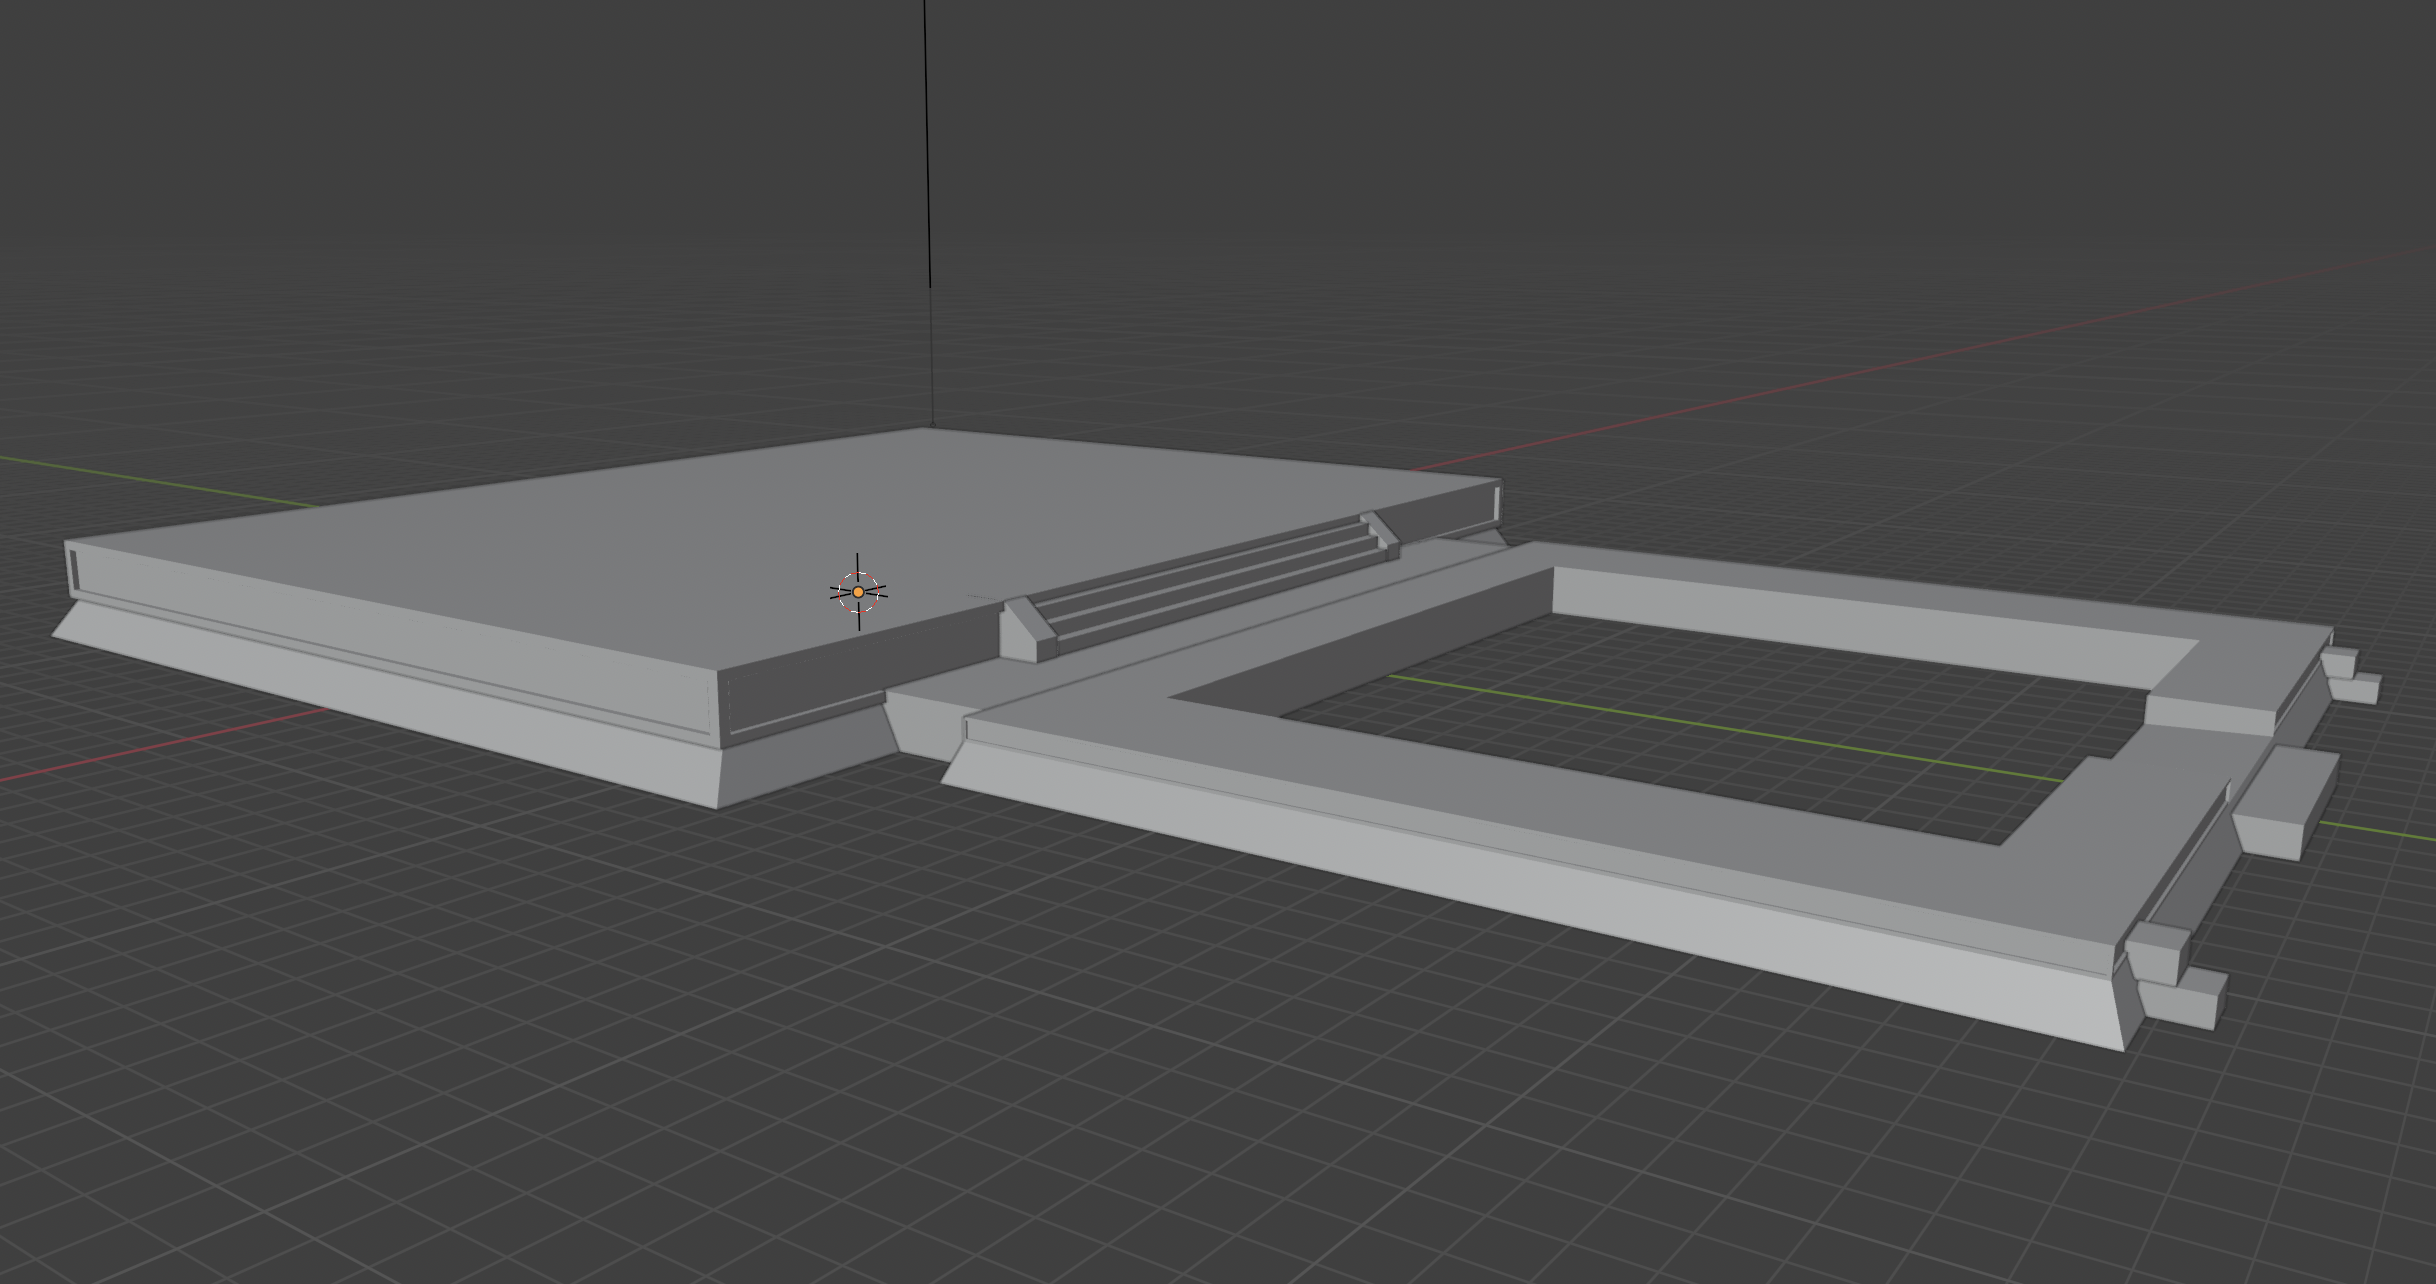
\includegraphics[width=0.85\linewidth]{resultados/figures/palangana/palangana_solid.png}
    \end{subfigure}

    \vspace{0.5em}

    % ----- Fila 2 -----
    \begin{subfigure}{0.48\textwidth}
        \centering
        \caption{Vista con materiales/texturas}
        \label{fig:palangana-textured}
        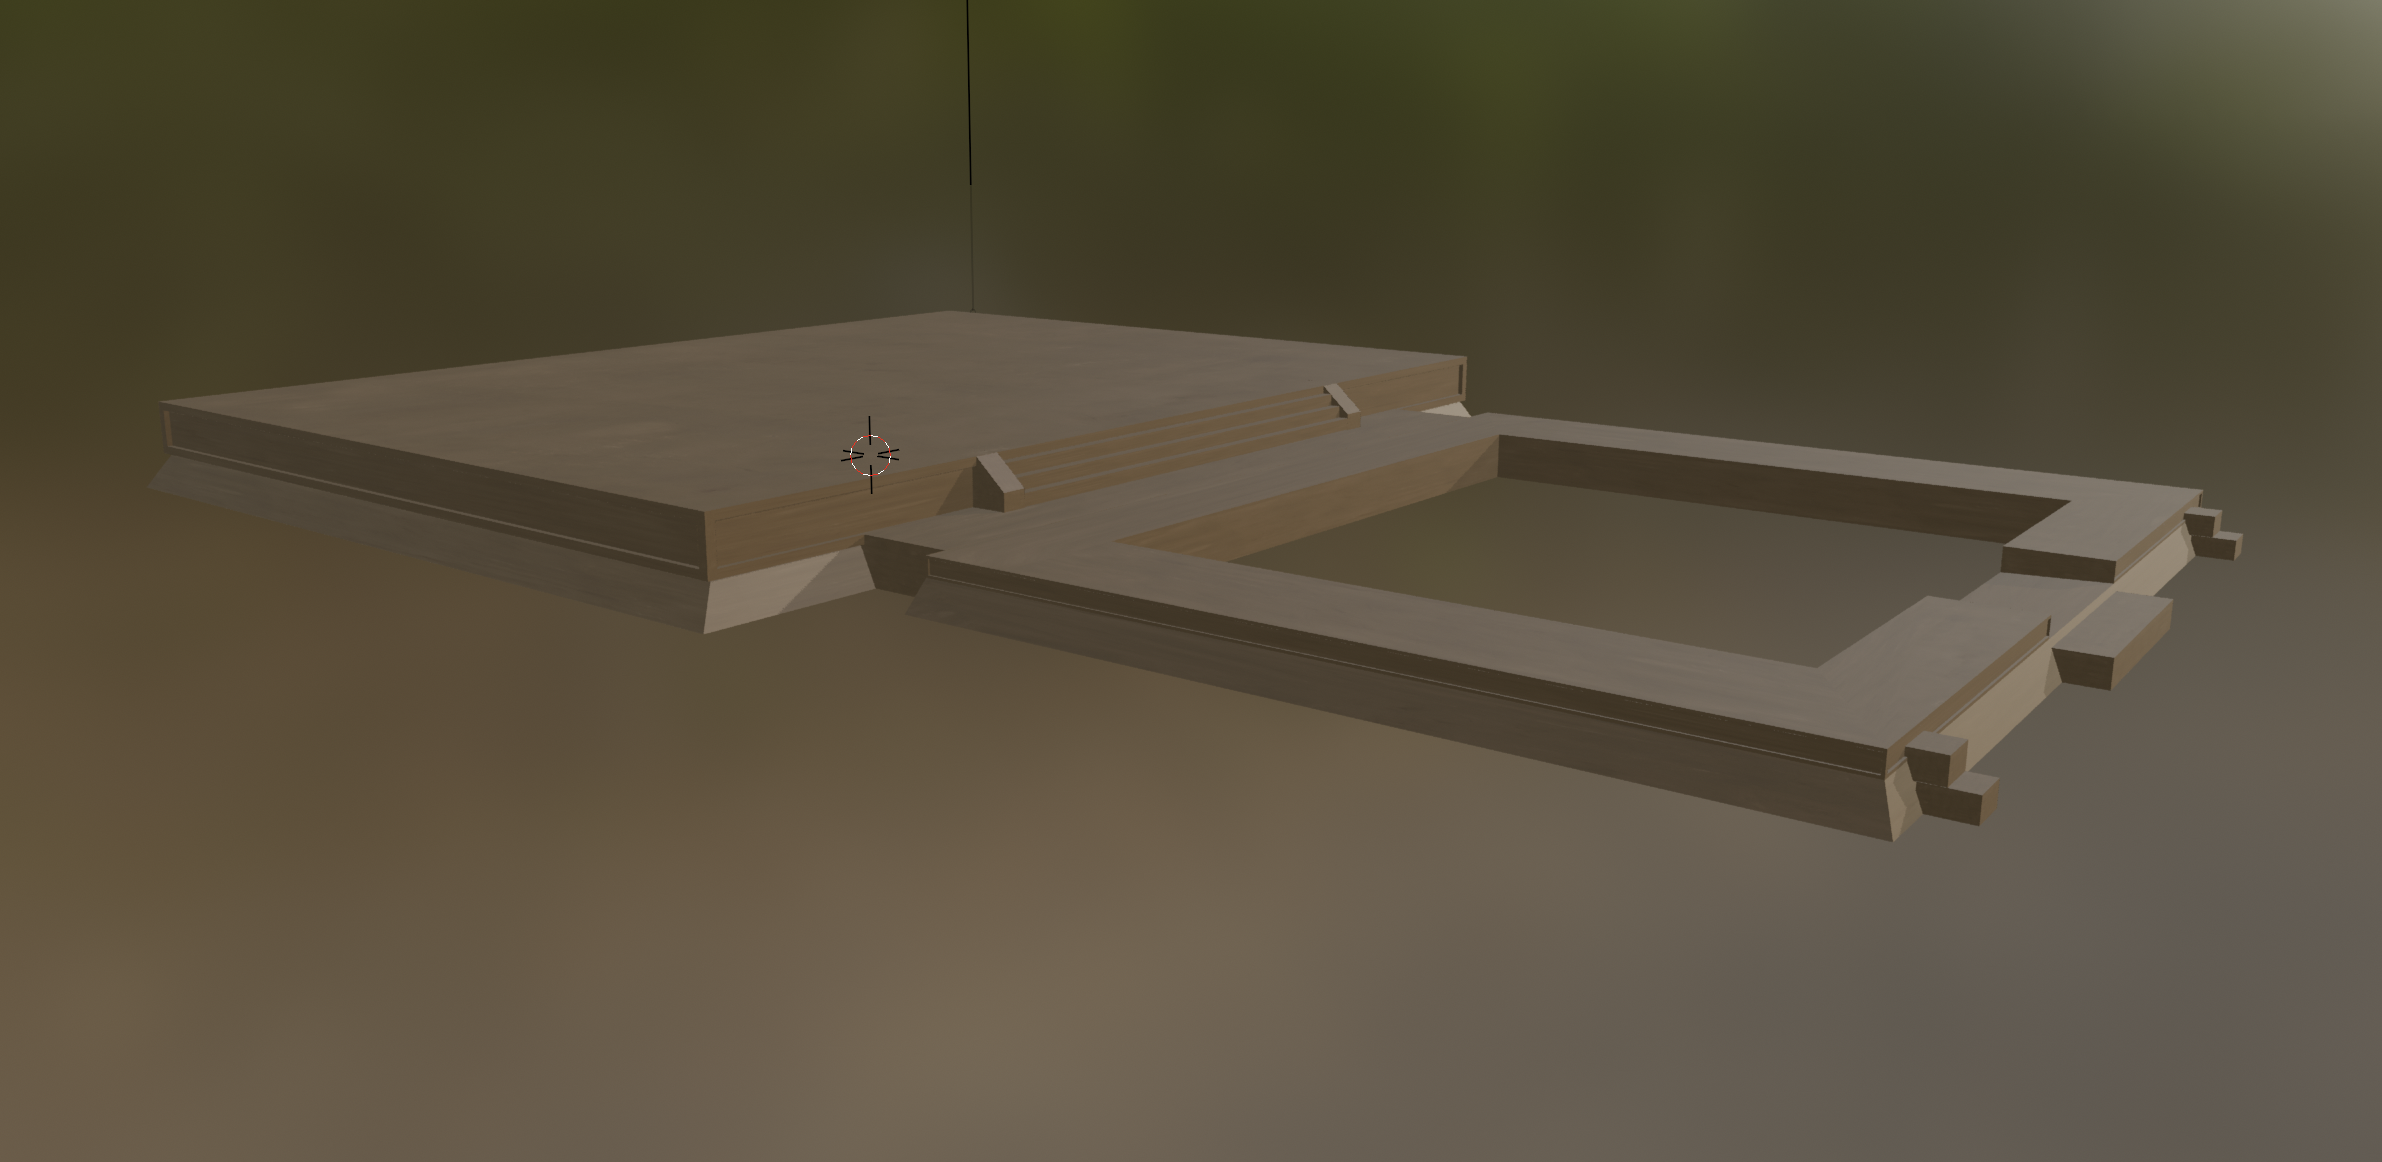
\includegraphics[width=0.85\linewidth]{resultados/figures/palangana/palangana_textured_viewport.png}
    \end{subfigure}
\end{figure}

\begin{figure}[!htbp]
    \centering
    \caption{Montículo La Palangana visualizado en la aplicación de realidad aumentada, mostrando la reconstrucción superpuesta en el entorno real del parque arqueológico}
    \label{fig:palangana-ar}
    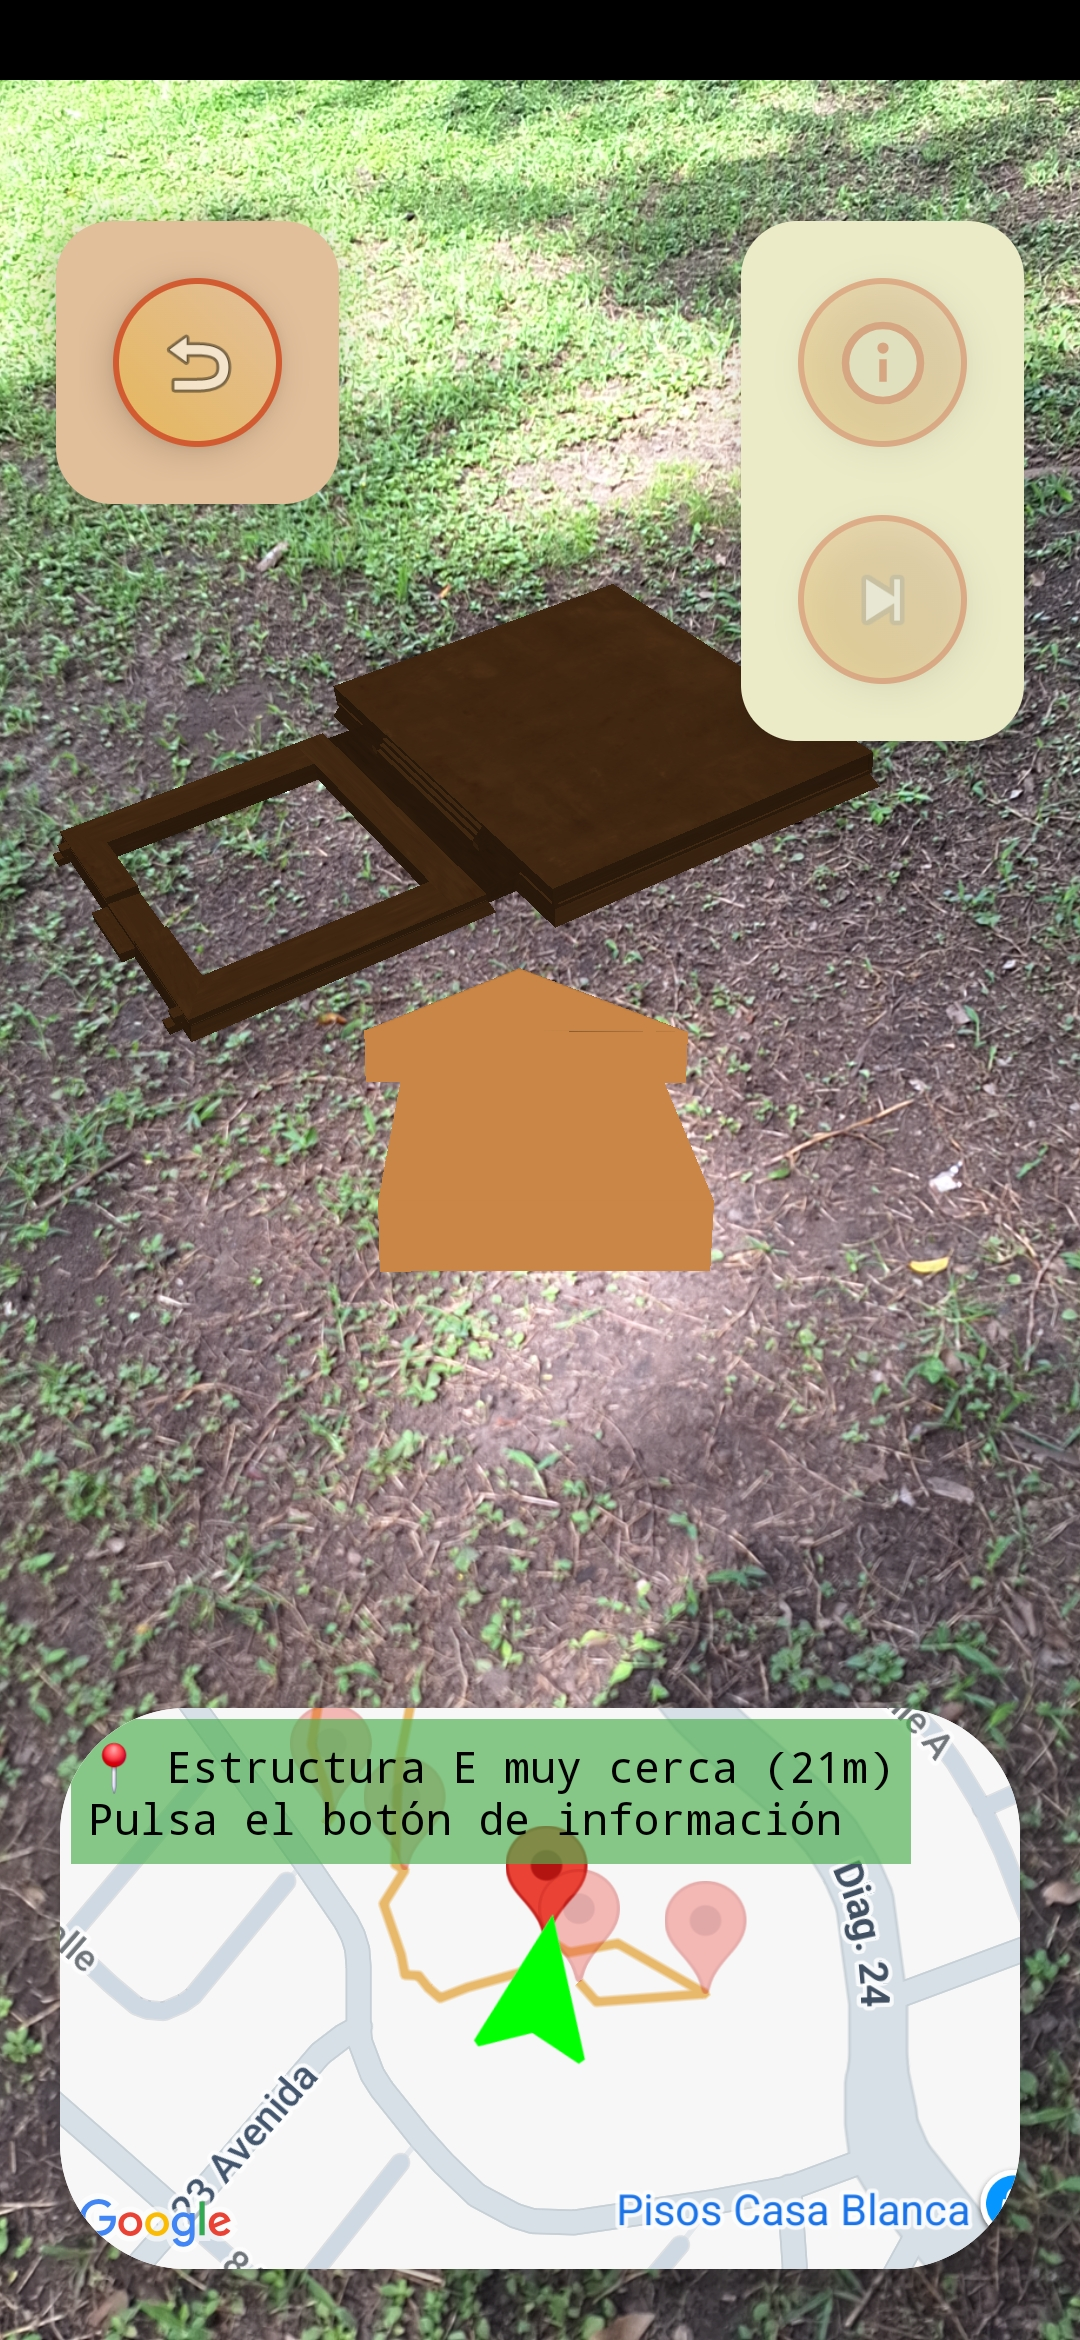
\includegraphics[width=0.28\linewidth]{resultados/figures/palangana/palangana_ar.jpg}
\end{figure}
\FloatBarrier
\clearpage

\subsection{Resultados de la encuesta}
\FloatBarrier

\begin{figure}[H]
    \centering
    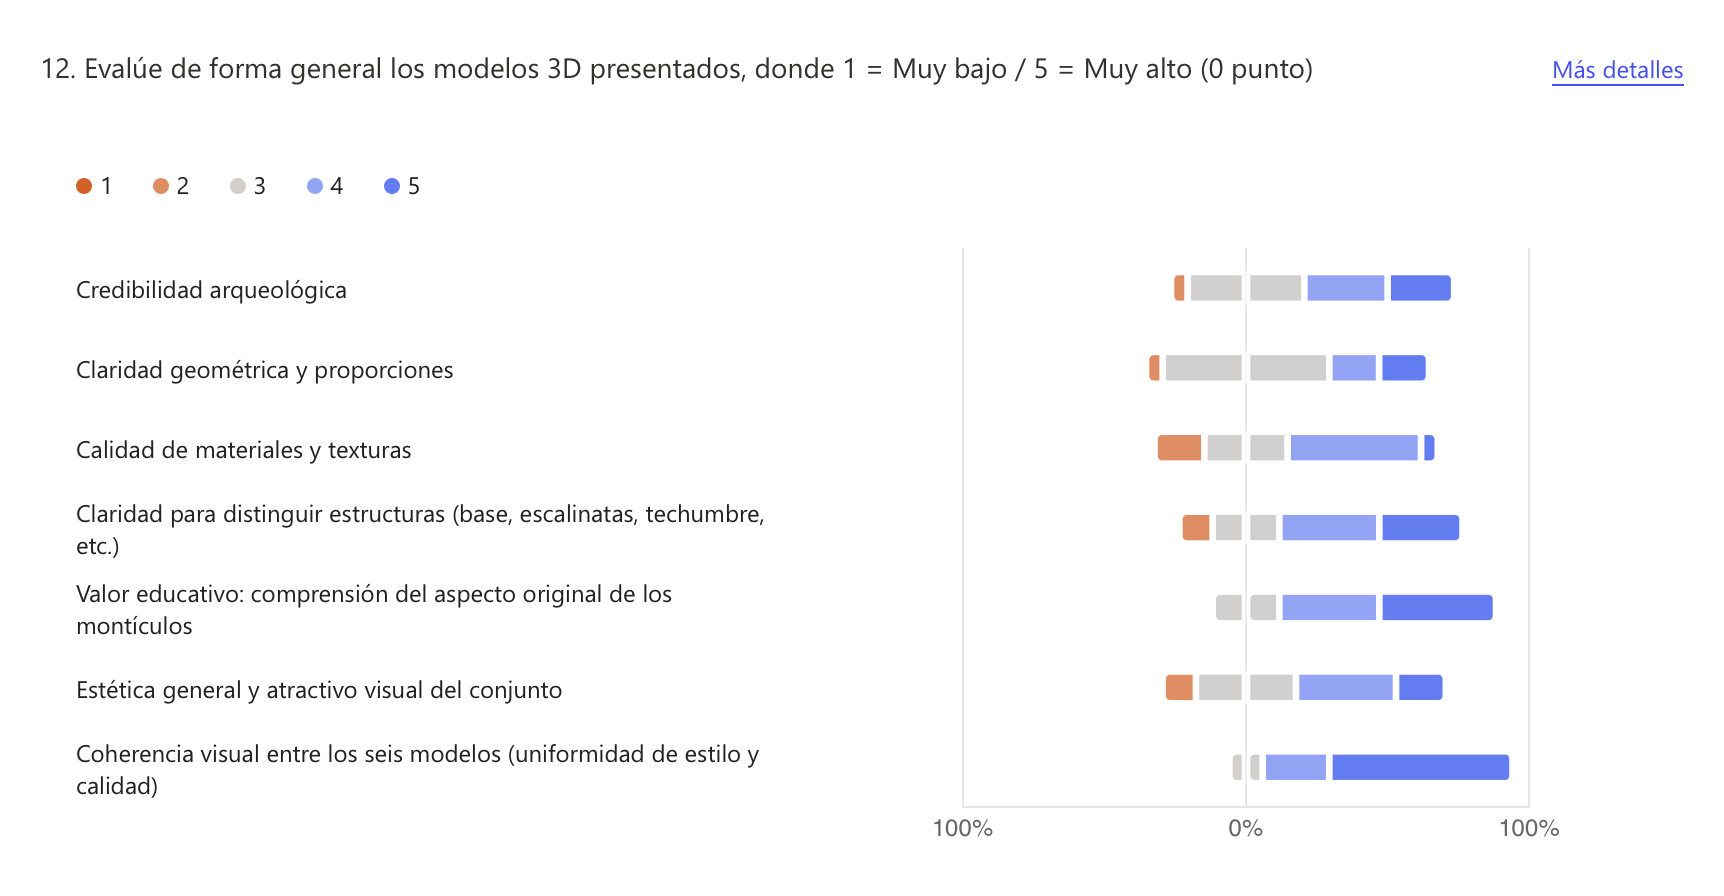
\includegraphics[width=\textwidth]{resultados/figures/Resultados_encuesta.png}
    \caption{Resultados de la encuesta aplicada a los usuarios.}
    \label{fig:resultados-encuesta}
\end{figure}


	\fi
\fi

% DISCUSIÓN DE RESULTADOS
% ------------------------------------------------------------------------------
\ifdefined\CAPanalisisderesultado
	\newpage
	\chapter{Discusión de resultados}
	\ifdefined\parpordefecto
		\defaultparformat{l-discusion}
	\else
		% l-analisis_de_resultados.tex
% !TEX root = z-main.tex

\section{Análisis de resultados}

Este capítulo discute el conjunto de modelos desarrollados (Montículos 3, 7, 12, 13, 14 y La Palangana), analizando el flujo de trabajo empleado y los resultados alcanzados en tres etapas: modelado geométrico, aplicación de materiales/texturas e integración prevista a un ambiente de realidad aumentada (RA). Se incluyen, además, consideraciones de validación arqueológica, rendimiento, limitaciones y líneas de trabajo futuro.

\subsection{Modelado geométrico}

Se completó el modelado tridimensional de los seis montículos propuestos siguiendo un procedimiento uniforme. El flujo por etapas (malla $\rightarrow$ sólido $\rightarrow$ texturizado) permitió validar progresivamente la calidad del resultado:
\begin{itemize}
    \item \textbf{Geometría base (wireframe).} Esta vista facilitó la inspección de proporciones, alineación de escalones, continuidad de taludes y simetrías. Fue útil para detectar y corregir aristas/caras innecesarias, evitar geometría y asegurar una topología limpia.
    \item \textbf{Volumetría (sólido).} La visualización sin materiales aisló la forma general de cada montículo y ayudó a comprobar la relación entre plataformas, escalinatas y superestructuras, así como la pendiente y los cambios de nivel.
    \item \textbf{Aplicación de materiales (texturizado).} En esta fase se verificó la correspondencia entre las texturas asignadas y los materiales originales documentados, cuidando la orientación y escala para obtener una representación realista.

\end{itemize}

\subsection{Texturizado y materiales}

La aplicación de materiales se orientó a reflejar acabados de barro, paja y maderas creíbles para Kaminaljuyú, manteniendo uniformidad visual entre modelos:
\begin{itemize}
    \item \textbf{Criterios visuales.} Se priorizaron gamas de barro en superficies expuestas, y tonos rocosos para bordes o elementos constructivos, siguiendo recomendaciones del área de Arqueología.
    \item \textbf{UV y repetición.} Se cuidó el desplegado UV para minimizar estiramientos perceptibles y favorecer patrones repetibles sin artefactos notorios en planos amplios (plataformas y taludes).
    \item \textbf{Preparación para RA.} La cantidad de materiales se mantuvo acotada para reducir mallas, y las texturas pueden consolidarse y emplear compresión en la exportación.
\end{itemize}

\subsection{Modelos en ambiente virtual (RA)}

Los modelos tridimensionales fueron preparados para su integración en un entorno de realidad aumentada en Android, en el cual podrán visualizarse superpuestos al espacio físico. Para facilitar su uso, cada modelo se exportó en formato \emph{.obj} con su correspondiente archivo \emph{.mtl}, manteniendo materiales simples y compatibles con los motores gráficos empleados en la aplicación. Se cuidó la orientación en los ejes y la ubicación del origen en (0,0,0), de modo que los modelos puedan escalarse y posicionarse con facilidad dentro del entorno virtual. Asimismo, se verificó la coherencia de escala entre los seis montículos y la uniformidad del estilo visual, garantizando una correcta correspondencia espacial y visual al momento de su despliegue en RA. Aunque la implementación de la aplicación corresponde a otro integrante del equipo, los modelos se entregaron optimizados y listos para su uso en dicha plataforma.

\subsection{Validación arqueológica y coherencia entre modelos}

El conjunto mantiene una lectura coherente con los rasgos registrados para Kaminaljuyú:
\begin{itemize}
    \item \textbf{Forma escalonada.} Las proporciones de plataformas y la relación con la escalinata principal son consistentes entre montículos, respetando las variaciones particulares observadas en cada caso.
\end{itemize}

\subsection{Comparación y síntesis del conjunto}

En conjunto, los seis modelos mantienen una coherencia formal y visual que refleja adecuadamente las características arquitectónicas de Kaminaljuyú. Todos fueron elaborados mediante el mismo flujo de trabajo, lo que permitió conservar la proporción entre plataformas, taludes y escalinatas, así como una topología limpia y eficiente gracias a la eliminación de caras no visibles. El resultado evidencia que el pipeline es reproducible y puede aplicarse a futuros montículos o variantes sin comprometer la consistencia general.

En términos de balance entre fidelidad y rendimiento, la simplificación geométrica se mantuvo dentro de límites adecuados para conservar los rasgos constructivos esenciales, garantizando al mismo tiempo un desempeño óptimo para su uso en entornos de realidad aumentada. Asimismo, la uniformidad de materiales y texturas, con excepción del Montículo 14, que requirió ajustes particulares, favorece la lectura visual del conjunto como parte de un mismo sitio arqueológico.

Finalmente, la representación tridimensional obtenida contribuye a propósitos educativos y de divulgación, al ofrecer una forma accesible y visualmente coherente de aproximarse a cómo pudieron verse originalmente las estructuras, facilitando su comprensión por parte del público general y de visitantes en experiencias de realidad aumentada.

\subsection{Limitaciones}

\begin{itemize}
    \item \textbf{Datos de partida.} Algunas suposiciones de materiales y acabado superficial son creíbles pero no definitivas, podrían refinarse con campañas de documentación adicionales.
    \item \textbf{Iluminación de referencia.} Las vistas de \emph{viewport} no equivalen a un render físicamente basado, el aspecto puede variar con condiciones de iluminación realistas en RA.
    \item \textbf{Detalle fino.} Elementos menores (erosión, irregularidades, grietas) fueron simplificados para priorizar legibilidad y rendimiento.
\end{itemize}

\subsection{Trabajo futuro}

\begin{itemize}
    \item \textbf{Afinar materiales PBR.} Incorporar mapas de normales y oclusión ambiental derivados de texturas reales o fotogrametría puntual para detalles finos.
    \item \textbf{Ampliación del corpus.} Extender el pipeline a otros montículos o variantes históricas y documentar discrepancias para análisis comparativo.
\end{itemize}

\section{Discusión de resultados}

Ver si se discute solamente lo de la encuesta o también lo de los resultados del modelado.
	\fi
\fi

% CONCLUSIONES
% ------------------------------------------------------------------------------
\ifdefined\CAPconclusiones
	\newpage
	\chapter{Conclusiones}
	\ifdefined\parpordefecto
		\defaultparformat{m-conclusiones}
	\else
		% m-conclusiones.tex
% !TEX root = z-main.tex


\section{Conclusiones}

El desarrollo de modelos tridimensionales del sitio arqueológico Kaminaljuyú permitió alcanzar los objetivos planteados y responder a la necesidad de contar con herramientas digitales que favorezcan la preservación y difusión del patrimonio arqueológico guatemalteco. La aplicación del modelado y la animación \gls{3d} demostró ser una estrategia efectiva para representar digitalmente estructuras que, en la actualidad, se encuentran ocultas o deterioradas, contribuyendo así a su conservación visual y educativa.

La fidelidad geométrica y la coherencia visual de los seis montículos modelados confirmaron la viabilidad técnica del proceso metodológico implementado. El uso del software Blender, junto con la validación arqueológica y la gestión digital colaborativa, garantizó resultados consistentes y replicables. La integración de texturas realistas mejoró la percepción visual de las estructuras, facilitando su comprensión por parte de los usuarios.

La evaluación de los modelos en entornos de realidad aumentada evidenció su efectividad como medio de exploración e interpretación arqueológica. Los usuarios y especialistas validaron su utilidad para visualizar el sitio en contexto y reconocieron el potencial educativo de la herramienta.

Los resultados alcanzados demuestran que la combinación de modelado tridimensional y realidad aumentada constituye un recurso tecnológico aplicable a la investigación, conservación y divulgación del patrimonio. El trabajo desarrollado sienta las bases para futuras implementaciones en otros sitios arqueológicos del país, promoviendo la digitalización y accesibilidad del legado histórico guatemalteco mediante herramientas tecnológicas contemporáneas.


	\fi
\fi

% RECOMENDACIONES
% ------------------------------------------------------------------------------
\ifdefined\CAPrecomendaciones
	\newpage
	\chapter{Recomendaciones}
	\ifdefined\parpordefecto
		\defaultparformat{n-recomendaciones}
	\else
		% n-recomendaciones.tex
% !TEX root = z-main.tex

\begin{itemize}
    \item Optimizar los materiales aplicados a los modelos tridimensionales mediante el uso de técnicas basadas en propiedades físicas (\gls{PBR}), con el fin de mejorar la respuesta a distintas condiciones de iluminación y aumentar el realismo visual en entornos de realidad aumentada.

    \item Realizar pruebas de visualización directamente en el parque arqueológico Kaminaljuyú, para evaluar el comportamiento de los modelos en su contexto original y ajustar parámetros de escala, orientación y desempeño en campo.

    \item Replicar la metodología de modelado tridimensional en otros sitios arqueológicos de Guatemala, adaptándola a las condiciones particulares de cada entorno y con el acompañamiento de especialistas en arqueología, diseño digital y educación patrimonial.

    \item Incorporar estrategias de accesibilidad digital y recursos educativos complementarios que permitan a los usuarios interactuar con el patrimonio de forma inclusiva, fortaleciendo el vínculo entre la tecnología y la preservación cultural.
\end{itemize}

	\fi
\fi

% BIBLIOGRAFÍA
% ------------------------------------------------------------------------------
\ifdefined\CAPbibliografia
	\newpage
	\clearchapter\phantomsection
	\chapter{\bibname}
	\printbibliography[heading=none]
\fi

% ANEXOS
% ------------------------------------------------------------------------------
\ifdefined\CAPanexos
	\newpage
	\chapter{Anexos}
	\ifdefined\parpordefecto
		\defaultparformat{p-anexos}
	\else
		\input{p-anexos}
	\fi
\fi

% GLOSARIO
% ------------------------------------------------------------------------------
\ifdefined\CAPglosario
	\newpage
	% Imprime el glosario con su propio encabezado (evita duplicar \chapter)
	\glsaddall
	\printnoidxglossary[title={Glosario}]
\fi

\end{document}